% !Mode:: "TeX:UTF-8"
\renewcommand{\b}{\boldsymbol}

\chapter{\TitlechapterI}
在复杂过程工业系统控制研究领域中,基于传统控制理论的系统辨识及控制器设计方法受限于系统复杂性难以适用。
而基于强化学习的无模型控制策略学习方法虽然不受系统复杂性的影响,但需要与环境之间不断进行交互反馈,因此同样不适用于试错代价极其高昂的工业场景。
模型预测控制方法首先构建被控系统的预测仿真模型,然后依赖于预测模型的推演结果实现系统优化及控制策略,有效解决了复杂系统的控制决策难题~\cite{Yuan2020,Member2019,wu2020optimization}。
随着大数据采集与处理技术的不断进步,很多企业会在复杂工业设备上安装大量传感器以监测工业系统的实时运行过程,
% 其中,数据驱动方法为建模复杂工业过程最常用的技术。
并利用采集到的数据集以数据驱动方法训练时序预测模型\cite{larsson2002identification}。
为了获得鲁棒、高精度的预测模型,需要对复杂工业系统的内在特性进行深入分析,大部分复杂工业系统通常具有以下典型特征:
\begin{itemize}
\item \textbf{非线性系统:}大多数工业系统的运行过程具有极强的非线性,而非简单的仿射系统或线性系统。
\item \textbf{系统的部分观测性}:一般情况下,从传感器或利用其他感知方法提取的系统信息是不完整的,导致这样的系统中存在许多未知的隐变量。
\item \textbf{长延迟的影响}:系统当前状态的变化受很长一段时间之前外部输入及内部状态的影响。
\item \textbf{连续时间演化}:由于真实的工业系统遵循各种物理规律,它们的时间演化可以用连续时间的微分方程表示。
\end{itemize}

对于上述复杂工业系统特点,许多工业界和学术界的研究人员通过构建不同预测模型来解决这些问题。
特别地,在基于数据的连续时间系统预测及辨识领域中,研究人员主要利用采样于真实系统的有噪数据来拟合高阶微分方程。
然而,这种方法不适用于建模部分可观测系统(Partially Observed System)和极端复杂的工业系统.
伴随着深度神经网络技术的不断发展,得益于其强大的特征表示能力和可扩展的参数结构,深度学习在解决复杂工业系统的预测及分析问题时被广泛使用。如时间序列预测~\cite{Member2019,Essien2020,9161367,9522017,neu2021systematic}、设备异常检测等~\cite{9326384}。
然而,现有的大多数基于深度学习的系统建模及预测方法都是基于离散时间域的,忽略了系统的连续时间特性。从模型结构与系统本体的一致性角度来看,忽视系统本身具备的连续时间先验特性会增加模型的自由度及拟合难度,最终限制了模型精度。
% The above features of a thickening system create challenges for predictive control. There are a number of studies addressing these challenges. 
% Data-driven methods are emerging as one of the most successful techniques for modeling complex processes~\cite{larsson2002identification}. 
% Traditional data-based CT system prediction methods focus on fitting high-order differential equations based on sampled noisy data from real systems. 
% However, they lack the ability to cope with partially observed and extremely complex system dynamics.
% Recent advances of deep neural networks (DNNs) have shown their strengths in addressing these issues owing to their strong feature representation abilities and scalable parameter structures, leading to the wide usage of DNNs in computer vision\cite{voulodimos2018deep,ma2020data, ma2021sesf}, natural language processing~\cite{young2018recent,9260162}, time series prediction~\cite{Member2019,Essien2020,9161367,9522017,neu2021systematic}, and fault diagnosis~\cite{9326384}. However, most DNN-based system-modeling methods are based on discrete time, disregarding the CT properties of a system. The lost prior information from physical insights undoubtedly leads to the deterioration of the model accuracy. 

% 另一方面,利用本章节所介绍的复杂系统预测模型,可以从两方面辅助系统控制的研究:
另一方面,复杂系统预测模型一般需要从两方面辅助系统控制的研究:
首先,模型的预测结果能够为基于模型的控制算法提供短期预测功能。如MPC方法中,预测模型提供了被控系统会如何受控制输入影响的先验知识,从而将系统最优控制近似为了序列优化问题。
其次,预测模型可以模拟系统在长控制输入信号下的系统输出~\cite{Demeester2020SystemIW},因此可以作为验证系统控制策略可行性的试错仿真场景。在复杂的过程工业系统控制领域中,验证控制器的性能和安全性是有极其必要的。
与短期预测相比,系统输出模拟需要预测模型有更高的稳健性和鲁棒性以提供长期的无反馈开环预测。
然而,在现有围绕工业系统预测的方法研究中,很少工作关注于如何设计预测模型以同时适用于短期和长期预测。
% ,进而服务于MPC控制及系统仿真。

% 针对上述工业系统存在的复杂特性以及长短期预测需求,本章节以ODE-Net作为模型骨架结构,从连续时间域角度拟合复杂工业系统的动态过程,由此提出了一种连续时间域
针对上述工业系统存在的复杂特性以及长短期预测需求,本章以ODE-Net作为模型骨架结构,
% 从连续时间域角度拟合复杂工业系统的动态过程,由此提出了一种连续时间域
提出一种由序列编码器、状态解码器和导数模块组成的深度连续时间(Continuous Time,CT)网络,以端到端的方式学习工业系统输出的自回归变化过程和输入对输出的非线性影响。
最终实现在给定历史系统运行轨迹及未来系统控制输入序列情况下,预测系统输出的未来变化。

% 因此,本章将以ODE-Net作为模型骨架结构,从连续时间域角度拟合复杂工业系统的动态过程,以实现给定历史系统输出序列及未来系统控制输入序列情况下,预测系统输出的未来变化。
具体地,由于工业系统往往存在长时间的系统延迟,因此本章节引入序列编码器以从历史系统运行轨迹中提取特征。
在预测时,本章提出方法构建了基于深度连续时间状态空间的导数模块。该模块相比于传统的离散序列模型,如循环神经网络(Recurrent Neural Network, RNN)等,更适用于建模系统在连续时间域下的非线性演化,并且在模块中通过引入隐状态可以辅助推断系统的不可观测信息。
最后,本方法将非平稳系统和平稳系统概念融入在模型的导数模块设计中,可以有效解决系统的短期和长期预测问题。
% 通过将历史系统轨迹和任意长度的系统输入输入到模型中,解决了短期和长期预测问题。然后预测未来的系统输出。
本章研究在工业系统预测领域有三个方面贡献:
%%%%%%%%%%%%%%%%%%%%%
\begin{itemize}
\item 提出了一种新的基于深度学习的工业系统连续时间预测模型。深度学习网络由三个部分组成:序列编码器、状态解码器和导数模块。
\item 基于平稳系统和非平稳系统概念,本章设计了两种导数模块,分别处理短期和长期预测任务。
\item 利用来源于某真实铜矿场中膏体浓密机的历史运行数据验证了本章提出方法的有效性。结果表明,该模型在预测具有非线性和高时滞特性的浓密机系统时具有较好性能。此外,本章节还进行了消融实验,以评估模型中每个模块的有效性。
\end{itemize}

本章节内容组织如下:
\ref{sec:formulate}节主要介绍了复杂输入输出系统预测问题的形式化表述并给出连续时间域下的状态空间模型表示方法。
% ~\ref{sec:model}节介绍了本章所述的连续时间深度预测模型。
\ref{sec:model}节主要介绍了基于ODE-Net的多输入输出工业系统连续时间预测模型,并分别介绍了序列编码器、导数模块以及状态解码器三大部分,同时给出了基于伴随状态的模型训练方法。
另外,该节分别面向短期预测和长期预测两种情况,介绍了两种导数模块定义方法。
% 同时给出了面向短期预测和长期预测的两种导数模块定义方法。
\ref{sec:3_interpolation_training}介绍了用于训练辨识模型的损失函数以及针对离散输入序列的可微并行插值方法。
% ~\ref{sec:derivative}节具体
% ~\ref{sec:interpolation}节具体介绍了用于连续化系统输入序列的并行插值方法。
% ~\ref{{sec:train}介绍了用于连续化系统输入序列的并行插值方法
% We next present the CT deep sequential model in Section~\ref{sec:CTDSM}. 
\ref{sec:case}节为实验章节,首先介绍了膏体浓密机系统预测问题以及数据集形式,然后对比了本章所述方法相比于其他时间序列预测模型的优势。最后通过消融实验探究了导数模块形式、序列编码长度、插值阶数对于预测效果的影响。
% 领域的其他模型,本章所述方法用于膏体浓密机系统预测问题的实验结果。
\ref{sec:conc}节对本章工作进行了总结,并展望了未来的研究方向。

\section{问题形式化描述}
\label{sec:formulate}
在复杂工业系统中,系统输出量定义为$\b y(k) \in \mathbb{R}^n$,
系统控制输入量定义为$\b x(k)\in \mathbb{R}^m$,其中$k$为采样时间点。
在诸多复杂工业场景中,系统输入对系统输出的影响本质上是非线性、高时滞的。且由于监测技术的限制,系统的一些关键参数无法获得,系统的观测空间往往是不完备的。
同时,观测数据会受到环境噪音以及系统本体中未知扰动的干扰。
% 此类复杂特性使得传统系统辨识方法\cite{larsson2002identification}或预测模型\cite{box2015time}难以对复杂工业系统进行有效的学习。
% 因此本章采用基于深度学习的黑箱数据驱动方法建模复杂系统的状态空间模型,使模型能够利用序列数据推断系统的隐状态。
因此需要从时序角度引入目标系统的历史信息以消除不完全观测带来的非确定性。
具体地,本章将系统预测问题建模为在已知未来系统输入和历史系统运行轨迹下估计未来系统输出。
% we formulate the problem as a sequential prediction structure with symbolic modules:
首先定义系统的历史输入序列为 $\boldsymbol X_p^{N_x}=[\boldsymbol x(-N_x),\boldsymbol x(-N_x+1), \dots, \boldsymbol x(-1)]$, 历史系统输出为 
$\boldsymbol Y_p^{N_y}=[\boldsymbol y(-N_y),\boldsymbol y(-N_y+1),\dots, \boldsymbol y(-1)]$,系统的未来输入为 $\boldsymbol y_f^{M}=[\boldsymbol y(0),\boldsymbol y(1),\dots,\boldsymbol y(M-1)]$,模型需要预测系统的未来输出$\boldsymbol Y_f^{M}=[\boldsymbol y(0),\boldsymbol y(1),\dots,\boldsymbol y(M-1)]$。
其中,$\boldsymbol X_f^{M}$之所以已知,是因为在模型预测控制及系统仿真问题中,系统输入是已知的。
序列预测问题可用如下符号及公式表示:
% we reformulate the thickening system prediction problem as a sequential prediction structure to improve the accuracy of multi-step predictions:
\begin{equation}
\label{equ:discrete_seq2seq}
\left\{
\begin{aligned}
&\boldsymbol{h}(0) = \mathcal{F}(\boldsymbol X_p^{N_x}, \boldsymbol{Y}_p^{N_y}), \\
&\boldsymbol{H^M} = D(\boldsymbol{h}(0), \boldsymbol {X}_f^{M}),\\
&\boldsymbol{y}(k) = g(\boldsymbol{h}(k)),
\end{aligned}
\right.
\end{equation}

模块$\mathcal{F}(\cdot)$ 用于估计初始隐状态 $\b h(0)$,该隐状态携带了历史序列 $\boldsymbol X_p^{N_x} \text{ 和 } \boldsymbol Y_p^{N_x}$的信息。
通过构建合理的模型$D(\cdot, \cdot)$,即可利用初始的隐状态以及未来的系统输入,估计完整的系统状态序列$\b H^M$。序列中的每个隐状态$\boldsymbol h(k)$携带了、或编码了系统在$k$时刻的系统信息。
另外,通过非线性函数$g(\cdot)$解码$\boldsymbol h(k)$即可得到估计的系统输出。
%%%%%%%%%%%%%%%%%%%%%%%
% seeking help: 我们扩展了\eqref{equ:discrete_state_space}中的单步预测到预测系统的序列输出. 被优化的loss 来源于整个预测序列各个位置loss的累计。
%We generalize the single-step prediction in \eqref{equ:discrete_state_space} to predicting sequential system outputs.
%The losses at all of the positions from predicted sequence are accumulated to construct complete supervised loss.
%Optimized loss is derived from the accumulation of losses at various positions in the predicted sequence.
% The loss function is optimized with grand total of the whole prediction sequence.
%%%%%%%%%%%%%%%%%%%%%%%
% For neural network based implementations, we sets  $M$ as a changeable parameter among training and inference phases. 

% 公式
% % \eqref{equ:discrete_seq2seq}类似于自然语言处理领域的Seq2Seq模型~\cite{Weiss2017Sequence},
% 将三个序列$\boldsymbol X_p^{N_x}$, $\boldsymbol{Y}_p^{N_y}$,和 $\boldsymbol {X}_f^{M}$映射为被预测的系统输出序列$\hat {\boldsymbol {Y}}_f^{M}=[\hat{\boldsymbol {y}}(1),\hat{\boldsymbol y}(2),...\hat{\boldsymbol y}(M)]$。
% 然后,相比于机器翻译等序列转换任务,输入输出系统预测任务要求对于$\boldsymbol{h}(k)$的计算只能依赖于$\{\boldsymbol h(i), i\leq k-1\}$和$\boldsymbol{X}_{f}^{k}=\{\boldsymbol x(i), i\leq k-1\}$,
% 这样的限制促使本章在模型框架设计时采用自回归系统。

为了在预测模型中构造合理有效的模块$D$,一种简单有效的解决方案是采用单步自回归的离散时间状态空间模型 \cite{4019326}:
% From the perspective of discrete-time setting, a thickening system with long time delay and incomplete observations can be formulated by a state space model~\cite{4019326} which introduces hidden state $\boldsymbol h(t)$:
\begin{equation}
    \begin{aligned}
\boldsymbol{h}(k)&=d\big(\boldsymbol{h}(k-1), \boldsymbol{x}(k-1)\big)\\
\boldsymbol{y}(k)&=g(\boldsymbol{h}(k)),
    \end{aligned}
\end{equation}
其中隐状态$\boldsymbol{h}(k)$将系统的历史轨迹编码为紧密、定长的向量。
控制输入对系统的影响可以看作是对系统当前隐状态的单步非线性变换。
当给定某一时刻输入$\boldsymbol{x}(k-1)$和上一时刻隐状态$\boldsymbol{h}(k-1)$时,模型可以立即预测新的隐状态$\boldsymbol{h}(k)$。
一些先前的研究~\cite{CHAI201661}~\cite{KIM2004403}表明,大部分过程工业系统的运行本质为物理变化或化学变化,系统的动态过程更适合建模为连续域下的微分方程。
因此,本章遵照工业系统的先验知识,构建参数化连续时间微分方程模型,以拟合隐状态的一阶导数:
\begin{equation}
    \label{equ:derivative_model}
%\small
    \dot{\boldsymbol h}(t) = d(\boldsymbol{h}(t), \boldsymbol x(t)).
\end{equation}
在此处,离散下标$k$被替换为连续时间下标$t$以表示$\boldsymbol{h}(t)$的变化为连续时间过程。
对于复杂系统的预测模型可以进一步表示为式\eqref{equ:discrete_seq2seq} 和式 \eqref{equ:derivative_model}。
本章的目标是利用收集得到的系统运行轨迹数据,对上述模型中的各个参数化模块进行学习,包括序列编码器$\mathcal{F}(\cdot)$、连续时间导数$d(\cdot,\cdot)$和状态解码器$g(\cdot)$。
\section{基于ODE-Net的多输入输出系统预测模型设计}
\label{sec:model}
本章采用集成的深度神经网络以参数化拟合式~\eqref{equ:discrete_seq2seq}和~\eqref{equ:derivative_model}。
图~\ref{fig:model_structure}展示了网络中包含的各个组件及其连接。
对于给定条件范围内的历史序列轨迹 $\boldsymbol{X}_{p}^{N_{x}}$ 和 $\boldsymbol{Y}_{p}^{N_{y}}$,以及预测范围 内的系统输入序列$\boldsymbol{X}_{f}^{M}$,模型输出$\hat{\boldsymbol{Y}}_{f}^{M}$以近似估计系统输出 $\boldsymbol{Y}_{f}^{M}$。
% We separately introduce a recurrent neural network (RNN) network to encode historical system trajectories to the initial hidden state and an ODE system to describe the state space model in the given time range.
\begin{figure}[t]
    \centering
    %\setlength{\abovecaptionskip}{-0.1cm} 
    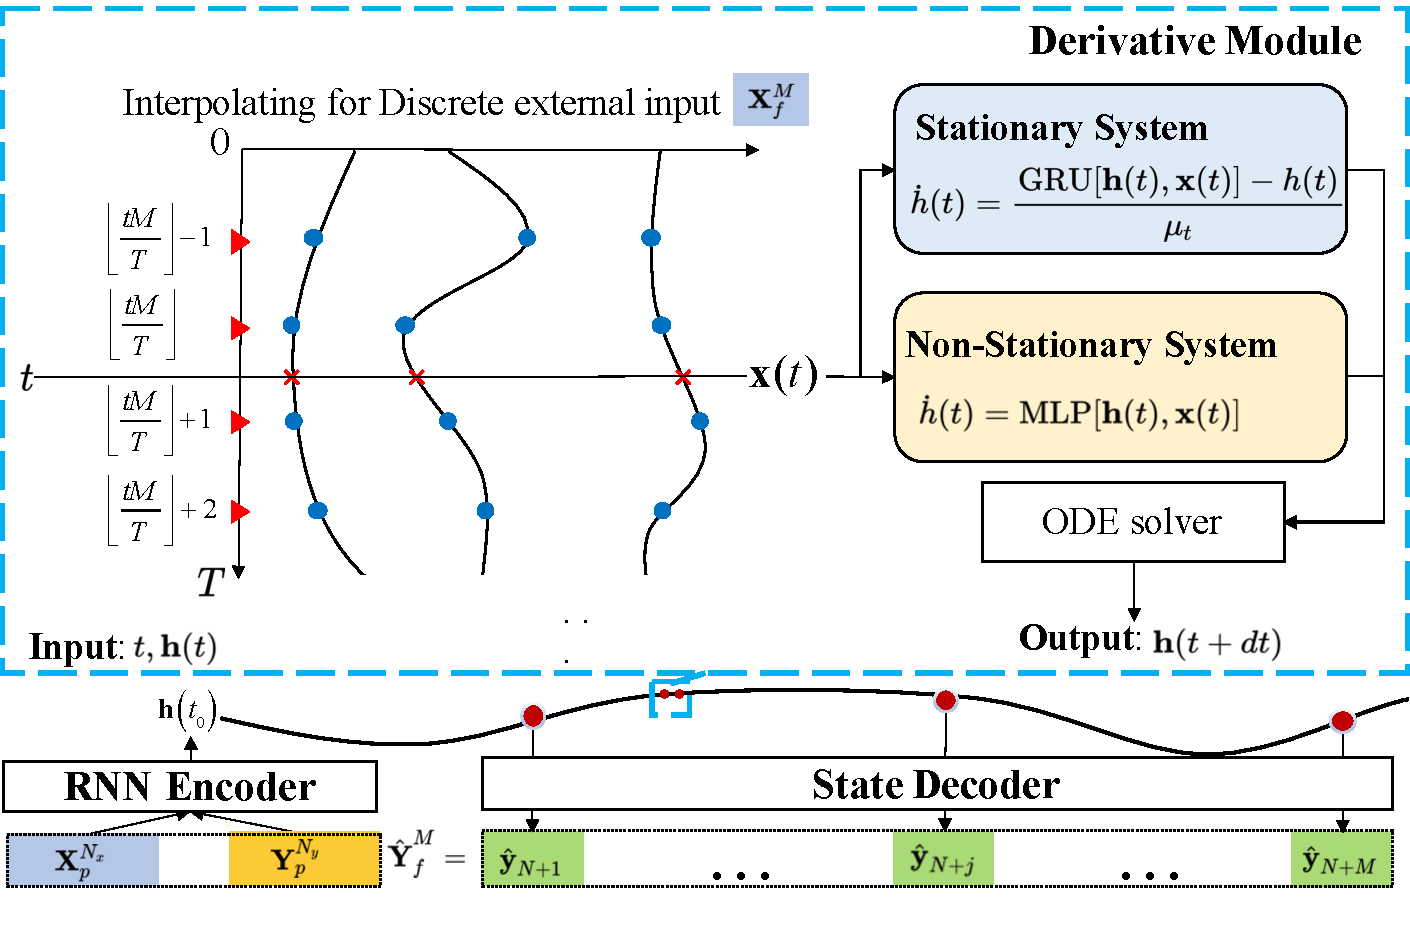
\includegraphics[width=1.0\linewidth]{figures/chapter3/model.pdf}
    \caption{
    基于ODE-Net模型的输入输出系统预测模型整体结构
    % The optimized loss is defined according to accumulative errors in the complete predicted sequence. 
    }
    \label{fig:model_structure}
%\vspace*{-0.4cm}
\end{figure}
该模型的预测过程分成以下几个步骤:
首先,采用基于循环神经网络的\textbf{序列编码器},将历史轨迹序列$\boldsymbol{X}_{p}^{N_{X}}$和$\boldsymbol{Y}_{p}^{N_{Y}}$编码为隐状态$\b h(t_0)$。

然后,将$\b h(t_0)$作为预测阶段待求解常微分方程的初始状态。
常微分方程的一阶导数由模型中的\textbf{导数模块}定义,模型将隐状态$\b h(t)$和连续时间域中任意时刻的外部控制信号$\b x(t)$作为输入,以估计隐状态$\b h(t)$的瞬时导数$\dot{\b h}(t)$。
模型中引入的\textbf{并行样条插值}模块将离散的外部输入序列$\boldsymbol{X}_{f}^{M}$插值为连续时间形式$\b x(t)$以作为导数模块的输入。
接下来,基于初始状态$\b h(t_0)$和导数模块定义的常微分方程,利用ODE求解器对微分方程进行求解可以得到时间范围$[t_0\leq t \leq t_M]$内的系统隐状态$\b h(t)$。
% 其中$[t_0,t_M]$代表与离线时间点序列$-1, \cdots, M-1$相对应的连续时间区间。
% The derivative of the hidden state with respect to the time variable $ \dot{\b h}(t)$ in the state space model is determined based on a neural network differential function $\b d(\b h(t), t)$. 

最后,模型利用多层感知器(MLP)网络构建\textbf{状态解码器},将求解出的隐状态$\b h(t)$映射为待预测的系统输出$\hat{\boldsymbol{Y}}_{f}^{M}$。
% We then provide a detailed introduction of each network module. 

下面,本章将详细介绍所述模型的每个模块的技术细节。


\subsection{利用历史序列编码器构建常微分方程初始状态}
% In our formulation\eqref{equ:discrete_seq2seq}, the input sequences consist of three parts:
% historical system output sequence $\boldsymbol{Y}_P^{N_y})$, historical system input sequence $\boldsymbol X_p^{N_x}$ and future system input sequence $\boldsymbol X_f^{M}$. 
由于大部分工业过程具有较长的时间延迟,因此系统的历史运行轨迹数据对于模型预测极其重要。本章引入了历史运行数据$\boldsymbol {X}_{p}^{N_{X}}$和$\boldsymbol {Y}_{p}^{N_{Y}}$作为模型输入的一部分。
具体地,利用基本的RNN模型,
将$\boldsymbol{Y}_p^{N_y}$和$\boldsymbol {X}_p^{N_x}$两个历史序列编码为某定长的隐状态,
以此推断常微分方程的初始值$\boldsymbol{h}(0)$ 。
\begin{equation}
\label{equ:rnn_encoder}
%\small
 \boldsymbol{h}(t_0) = \boldsymbol{h}(0) = f_{\text{RNN}}(\boldsymbol{Y}_P^{N_y},\boldsymbol X_p^{N_x},\theta _f),
\end{equation}
对于一般的工业系统,可以根据生产经验估计其系统时延为$T_d$,数据采样间隔为$T_s$,$N_y$和$N_x$可以近似估计为$N_y = N_x = N = T_d/T_s$。
% The influence of parameter $N$ on the model accuracy is examined in Section~\ref{sec:case}. 
% \begin{equation}
%     \label{NYNX}
%     N_y = N_x = T_d/T_s
% \end{equation}
在大部分工业系统中,当前系统状态与短期内的历史轨迹之间的互信息更大。
也正是因为该性质,本章利用了RNN的遗忘特性,并将其用于编码系统的历史轨迹。
利用序列编码器得到的隐状态$\b h(t_0)$编码了历史系统轨迹中对于预测所需的信息,该状态将作为待解ODE-Net的初始状态。

\subsection{利用可微常微分方程网络构建系统状态空间模型}
\label{sec:ODE-Net}
本小节将采用参数化的连续时间状态空间模型表示系统输入、隐状态和输出之间的关系:
\begin{equation}
    \begin{aligned}
     \dot{\boldsymbol h}(t)&=d(\boldsymbol{h}(t), \boldsymbol{x}(t), \theta _d),\\
\boldsymbol{y}(t)&=g(\boldsymbol{h}(t)).
    \end{aligned}
    \label{equ:ct_state_space}
\end{equation}
状态空间模型中将系统状态表示为定长的编码向量$\b h(t)$,
隐状态$\b h(t)$表征了系统的长时延特征以及非确定性。将原始的非马尔科夫系统转换为以$\b h(t)$所在状态空间的为核心的马尔科夫系统。

对于长度为$M$的待预测序列,本章在整数离散索引$[0,1,\dots,M]$和连续时间范围$[t_0\leq t_k \leq t_{M}]$之间构造双向映射。
给定初始状态为$\boldsymbol{h}(t_0)$,每个$\boldsymbol{h}(t_k)$为ODE方程在$t=t_k$处的解。
为了构造可学习的微分系统,本章使用可微ODE-Net~\cite{NIPS2018_7892}学习上述状态空间模型。

对于由某一预测评价指标确定的标量损失函数$L(\cdot)$,
其输入$\b{h}(t_k)$为ODE方程在$t=t_k$时刻的解。将ODE求解器表示为$\operatorname{ODESolve}$,我们有
\begin{align}
\label{equ:loss_ode_solver}
% \begin{aligned}
L\left(\boldsymbol{h}\left(t_{k}\right)\right)&=L\left(\boldsymbol{h}\left(t_{0}\right)+\int_{t_{0}}^{t_{k}} d(\boldsymbol{h}(t), \boldsymbol x(t), \theta_d) d t\right)\nonumber\\
&=L\left(\operatorname{ODESolve}\left(\boldsymbol{h}\left(t_{0}\right), d, t_{0}, t_{k}, \theta_d \right)\right).
% \end{aligned}
\end{align}
本章待求解的常微分方程是参数化的,
为了训练参数$\theta _d$以最小化$L(\cdot)$,需要根据上式计算损失函数对模型参数的梯度$\partial L / \partial \theta _d$。
此处需要引入伴随状态(Adjoint state),即损失函数对隐状态的梯度$\boldsymbol{a}(t)=\partial L / \partial \boldsymbol{h}(t)$.

利用链式法则可以证明任一时刻的伴随状态可由另一个ODE描述~\cite{NIPS2018_7892}:
\begin{equation}
\label{equ:ode_at}
\frac{d \boldsymbol{a}(t)}{d t}=-\boldsymbol{a}^{\top}(t) \frac{\partial d(\boldsymbol{h}(t), \boldsymbol x(t), \theta_d)}{\partial \boldsymbol{h}(t)}.
\end{equation}
依赖于伴随状态,损失函数 $L(\cdot)$对参数$\theta _d$的梯度可以通过求解第三个常微分方程得到:
\begin{equation}
\label{equ:grad_ode}
\frac{\partial L}{\partial \theta _d}=-\int_{t_0}^{t_{M}} \boldsymbol{a}^{\top}(t) \frac{\partial d(\boldsymbol{h}(t), \boldsymbol x(t), \theta _d)}{\partial \theta_d} d t.
\end{equation}
在确定的网络结构$d$和参数$\theta _d$下,
任意的ODE数值求解方法,如欧拉法(Euler)、中点法(Mid-point)和龙格-库塔法(Runge Kutta),均可同时求解三个微分方程,进而获得$\b h (t)$、$\alpha (t)$和${\partial L}/{\partial \theta}$在任意时刻的解。
一般情况下,在使用数值方法求解常微分方程时,具有较低误差容忍度的ODE求解器会增加调用微分函数$d$的频率。
造成更多的时间消耗,但其估计结果具有更高的准确性。
当使用神经ODE网络建模时间序列数据集时,这个准则同样是成立的。在实验环节,本章也探讨了不同微分方程求解器对于预测精度和消耗时间的影响。
时间成本和准确性的详细比较见~\ref{sec:case}节。

对于给定时刻ODE-Net输出的状态$\b h(t)$,需要使用状态解码器将其转换为系统的预测输出。
本章采用的状态解码器为普通的多层感知机网络:
\begin{equation}
    \hat{\boldsymbol y}(t) = \boldsymbol{V}^{\top} \tanh \left(\boldsymbol{W}\boldsymbol{h}_{t}+\boldsymbol{b}_{w}\right)+\b b_{v}.
\end{equation}
% A neural network with single hidden layer composed with learnable input layer ($\boldsymbol{W}$,
% $\boldsymbol{b}_w$) and hidden layer($\boldsymbol{V}$, $\boldsymbol{b_v}$) is utilized to predict the system output.
一般的状态空间模型多使用普通的矩阵变换以构建编码空间到系统输出空间的映射。本章中,由于公式
~ \eqref{equ:3_non_stationary}中的累加形式使输入$\b h(t)$的范围是非确定的,而实际系统的输出空间是有界的,因此选择带有$\tanh$非线性归一化的解码器以保证状态解码器的输出在合理的范围内。



\subsection{面向不同预测时长需求的常微分方程导数模块定义}
\label{sec:derivative}
\ref{sec:ODE-Net}节介绍了ODE-Net的求解和网络参数梯度的求解方法。
在本节中,将具体探讨ODE网络的结构细节。
最基本的ODE-Net模型采用普通的多层感知机神经网络估计状态导数\cite{chen2018neural},本章将此模型称为非平稳模型:
% We name 
% In this paper, the structures of derivative module $d$ are categorized into two types~\cite{Demeester2020SystemIW}: 
%non-stationary system or stationary system as follows:
% \begin{equation}
% \label{equ:3_non_stationary}
% d\left(\boldsymbol{h}(t), \boldsymbol{x}(t), \theta_{d}\right)=RNN\left(\boldsymbol{h}(t), \boldsymbol{x}(t), \theta_{d}\right)
% \end{equation}
\begin{equation}
\label{equ:3_non_stationary}
d\left(\boldsymbol{h}(t), \boldsymbol{x}(t), \theta_{d}\right)=\text{MLP}\left(\boldsymbol{h}(t), \boldsymbol{x}(t), \theta_{d}\right)
\end{equation}
该结构与普通的残差网络(ResNet)有很强的相似性。
在随机过程分析领域,非平稳系统指时间序列各个时刻的统计量(如均值和方差)随时间变化的随机过程~\cite{GUIDOLIN2018113}。
一般来说,复杂工业系统的输出往往属于非稳定时间序列,带有较强的趋势性。
差分操作~\cite{christoffersen2001forecasting}是一种消除序列趋势和季节性的有效方法。
该操作计算原始序列相邻位置之间的一阶差分或多阶差分,形成的差分序列往往是平稳的,更易于模型学习。
在预测阶段,将模型的预测结果进行积分即可复原为原始的非稳定序列。
在公式\eqref{equ:3_non_stationary}中,导数模块本质上学习了隐空间中隐状态的一阶差分。
相比于ARIMA模型等直接对系统输出进行差分,面向隐状态的差分模型具有同等或更强的表示能力,进而能够建模更高阶的非平稳系统。

然而,非平稳系统\eqref{equ:3_non_stationary}在处理长期预测任务时也面临着严重的问题。
在长时区间内求解ODE-Net时,对连续时间域内隐状态导数的不断积分会导致隐状态的值域范围显著扩增。
% 因此,模型的估计误差会相应增大,导致解码器难以准确地估计系统输出。
假设ODE-Net的预测误差服从白噪音分布$\mathcal{N}(0,\delta)$,经过时间$t_M-t_0$之后的累积误差服从分布$\mathcal{N}(0,(t_M-t_0)\delta)$。
由此可见,在预测长度足够长时,模型预测的误差将被持续累积,解码器难以准确地估计系统输出。

为了解决上述非稳定结构带来的误差累积问题,本章设计了一种基于平稳系统的导数模块形式,以处理模型的长期预测问题。
具体地,其隐状态导数定义为:
%Inspired by the \emph{Differencing} operation, another architecture of derivative module named stationary system is proposed to improve the stability in long-term prediction tasks:
\begin{equation}
\label{equ:stationary}
d\left(\boldsymbol{h}(t), \boldsymbol{x}(t), \theta_{d}\right)=\frac{1}{\mu _t}(\text{GRU}\left(\boldsymbol{h}(t), \boldsymbol{x}(t), \theta_{d}\right)-\b h(t))
\end{equation}
其中$\text{GRU}$表示门控循环单元。
对于无穷小时间步$\text{d}t$,可得:
\begin{equation}
    \lim_{\text{d}t \rightarrow 0}\boldsymbol{h}(t+\text{d}t) =(1-\frac{1}{\mu _t})\boldsymbol{h}(t)+\frac{1}{\mu _t}\text{GRU}\left(\boldsymbol{h}(t), \boldsymbol{x}(t), \theta_{d}\right)
\end{equation}
平稳系统能够根据当前外部输入$\b x(t)$和隐状态$\b h(t)$确定隐状态的移动目标点。
隐状态$\b h (t)$将始终朝向GRU网络输出的目标值移动,
其中,因子$\mu_t$规范了到达该目标的速度。
同时,由GRU网络的特性可知,其输出范围始终在$(-1,1)$中。
% It also restricts when $\b h_t$ moves toward GRU output.
因此无论微分方程求解时间区间有多大,求解ODE方程得到的任意时刻隐状态的解也在$(-1,1)$中,更便于解码器模块构建从隐空间到系统输出空间的稳定映射。
在长期预测任务中,相比于非稳定系统,这一特性能够显著地提升模型预测的准确性与稳定性。
% ,我们主要将其用于长期预测。
由于GRU具有较强的携带长时间信息的能力,所以我们使用GRU网络来构造导数模块。

考虑到非稳定系统和稳定系统的在不同的预测长度各有各的优势,本章将非平稳系统应用于短期预测,将平稳系统应用于长期预测。
% 对于非平稳系统中,主要将其用于短期预测。
% 由于隐状态导数的连续累积,隐状态的变化类似于维纳过程,将会在无约束的范围内不断扩散。
% 而GRU、LSTM等网络均假设模型输入应限定在有界范围内。因此,
% 本章在非稳定系统中利用MLP模块学习给定$\b h(t)$和$\b x(t)$下$\dot{\b h}(t)$的一阶导数。
\section{离散输入序列的可微并行插值方法及模型训练}
\label{sec:3_interpolation_training}
% 在式\eqref{equ:3_non_stationary}和\eqref{equ:stationary}中,$\dot{\b h}(t)$的计算依赖于连续的外部输入信号$\b x(t)$,而
在求解ODE-Net时,需要在连续时间域内给定任意时刻的系统外部输入值$\boldsymbol x(t)$,
而训练数据中的外部输入序列$\boldsymbol X_f^M$是离散采样的。
因此,在网络前向传播之前,需要将离散的外部输入序列转换到连续时间域中。

训练深度神经网络时,通常需要利用图形处理单元(GPU)的并行计算能力,将数据批量地送入模型并进行参数更新。这要求模型中的所有运算操作能够并行执行。
因此,本章基于标准的样条插值算法,实现了一种可微且并行的样条插值算法,能够将批量输入的离散序列并行地插值为连续时间信号。

不失一般性地,本节假设系统输入的维度$m$为1。
给定输入序列的批(batch)为:
$\b X = [\b x ^1, \b x ^2,\cdots\b x^B]$,其中$B$为批大小。
每个向量$\b x^i=\left[x_1^i, x_2^i, x_M ^i\right]$
为独立的输入序列,由$M$个采样数据组成,相邻数据点之间的采样间隔是一致的。
假定与$M$个采样点相对应的常微分方程求解时间区间为$[0,T]$。
% 对于任意给定的时间索引$T$,在这个间隔中约束为$0\leq T \leq T$。
对于任一给定的时间索引$t$,$0\leq t \leq T$,我们希望并行化地估计$\b X(t) = [\b x ^1(t),\b x ^2(t),\cdots,\b x^B(t)]$。
为了实现这一目标,首先构造从连续时间点到离散下标的转换。定义$k=\lfloor \frac{tM}{T} \rfloor$,给定$n+1$个数据点,$\{(k, \b x_k),(k+1, \b x_{k+1}),\cdots,(k+n, \b x_{k+n})\}$
可以计算时间$t$局部的$n$阶样条插值函数的系数矩阵$\b A\in\mathbb{R}^{(n+1)\times B}$:

% 首先,在区间$[0,t]$中,找到最接近$t$的且在$\{1,\cdots,M\}$中出现的整数索引$k=\lfloor \frac{tM}{T} \rfloor$。
\begin{equation}
\boldsymbol{A}=\left[\begin{array}{ccc}
k^{0} & \cdots & k^{n} \\
(k+1)^0 & \cdots & (k+1)^{n} \\
\vdots & \ddots & \vdots \\
(k+n)^0 & \cdots & (k+n)^{n}
\end{array}\right]^{-1}\left[\begin{array}{ccc}
x_{k}^{1} & \cdots & x_{k}^{B} \\
x_{k+1}^{1} & \cdots & x_{k+1}^{B} \\
\vdots & \ddots & \vdots \\
x_{k+n}^{1} & \cdots & x_{k+n}^{B}
\end{array}\right].
\end{equation}
一批数据中,所有离散序列在$t$时刻的插值为:
\begin{equation}
\left[ x^1(t), x^2(t),\cdots, x^B(t)\right]= \Bigg(\left[ 1, \frac{tM}{T},\cdots, (\frac{tM}{T})^n\right]\boldsymbol{A}\Bigg). 
\end{equation}
在一般的深度学习框架中,上述矩阵乘法和求逆矩操作可以高效地并行实现。
由于上述并行插值过程以及模型中的编码、解码以及常微分方程求解过程都是可微的,本章采用标准的反向传播算法训练完整模型,损失函数定义为标准的均方误差损失函数:
\begin{equation}
\label{equ:mse_loss}
\mathcal{O}\left(\hat{\boldsymbol Y}^M, \boldsymbol{Y}^M\right)=\frac{1}{M} \sum_{i=1}^{M}\left|\boldsymbol y_{i}-\hat{\boldsymbol y}_{i}\right|^2.
\end{equation}
% For uneven case, the interval time for sampled data is not constant.
% An obvious way is employing any interpolation method to pad the original data and produce a sequence with even time separation before training.
% Furthermore, some frequency domain based method could also produce continuous-time sequence from the discrete. 
% But we did not employ such methods because these methods only reserve the low frequent information and destroy the original sequence on discrete integral points.
% %and produce a new one.
% For example, the butterworth filter, a kind of low pass filer, will produce $x(t)\neq x_i$ when $\frac{tM}{T}=i$. 
% While the spline interpolations can avoid this problem.
% The experiment section will show the influence from the choice of the order in spline interpolation.

\section{实验验证与分析}
\label{sec:case}

\begin{figure}[t]
%\setlength{\abovecaptionskip}{-0.1cm} 
\centering
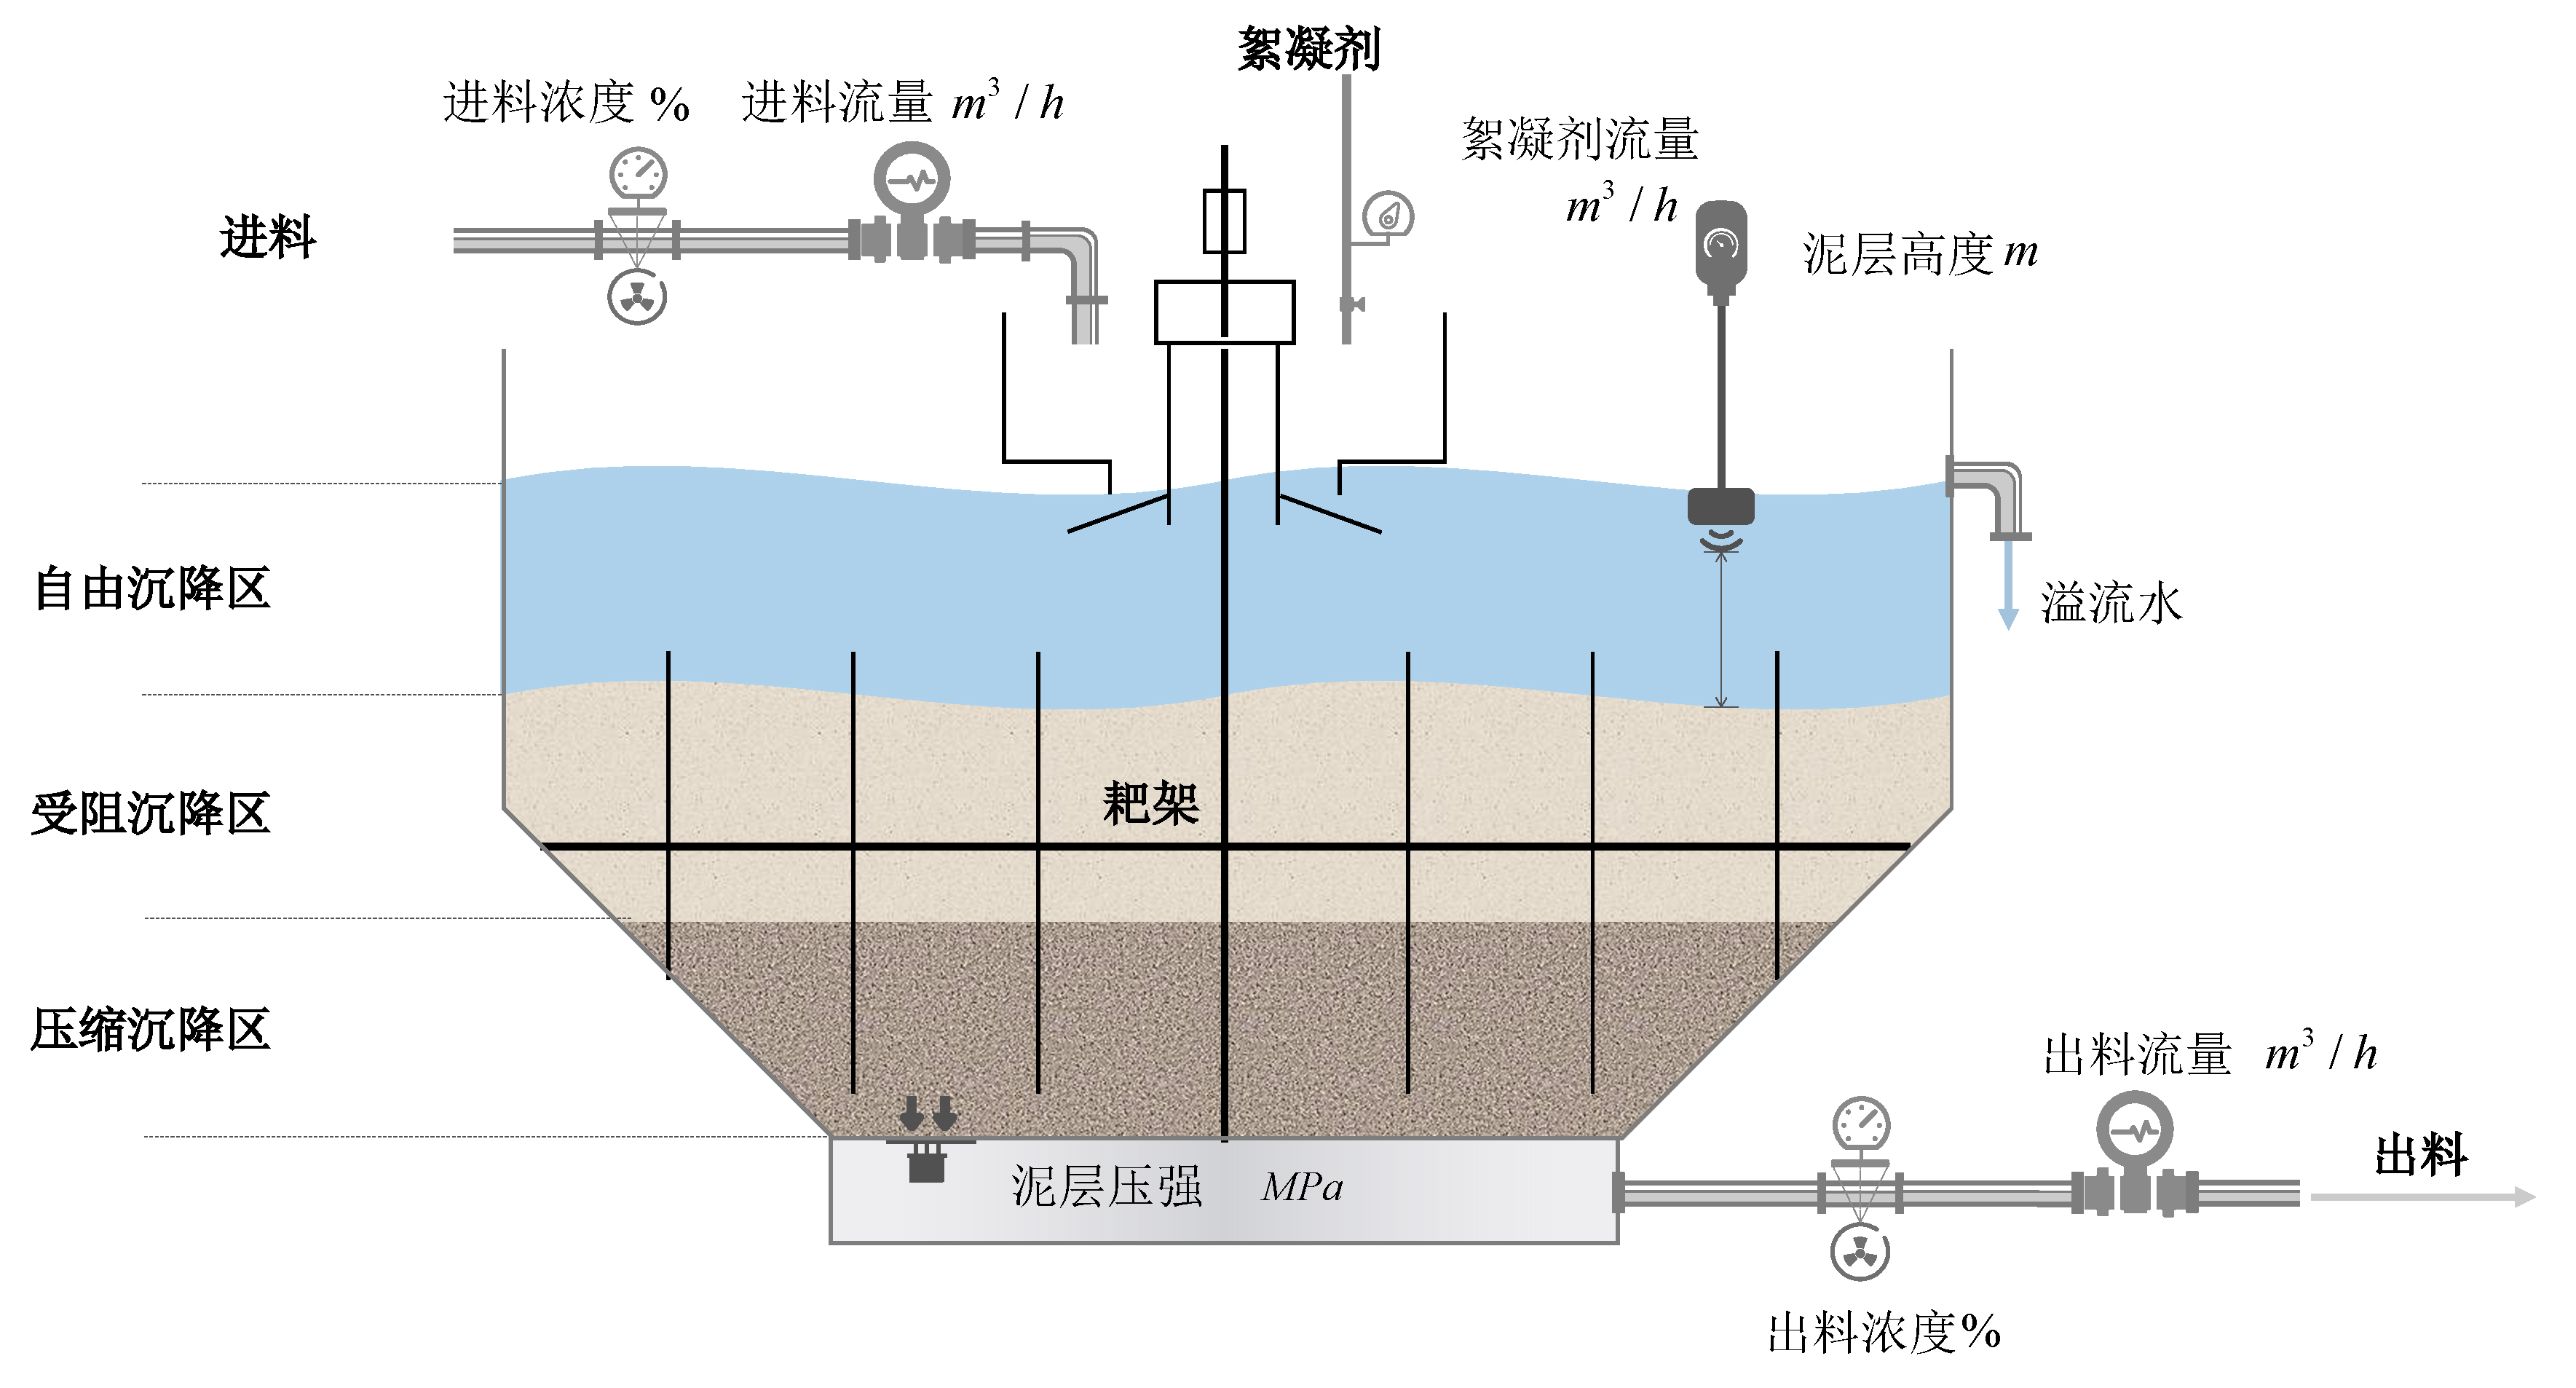
\includegraphics[width=\linewidth]{figures/chapter3/thickener.pdf}
\caption{
%%%%%%%%%%%%%%%%%%%%%%%%%%%
% seeking help: 如图所示,在实验的充填站,共有两台深锥浓密机,其中一主用,一备用,本章实验数据全部来源于第一台主用设备。
%As the figures illustrate above, there are two identical paste thickeners in the experimental backfilling station. One of them is primary device and the other is a spare. All of the original dataset in experiments are exported from the primary one.
膏体浓密机系统运行过程及监测变量图示
% The training data we use in this paper is collected from the primary device.
}
%%%%%%%%%%%%%%%%%%%%%%%%%%%
\label{fig:nfca_thickener}
%\vspace*{-0.3cm}
\end{figure}

% This section presents experimental results for the proposed method on the dataset of real thickening systems.
本节将采用真实工业系统数据对所提出的基于常微分方程网络的系统建模方法进行验证。
实验主要探究三个问题:
\begin{itemize}
\item \textbf{问题1}:相比于直接采用离散时序预测模型,使用深度连续时间网络和高精度ODE求解器建模预测工业系统能否获得更优的效果?
\item \textbf{问题2}:在不同预测长度下,使用平稳系统和非平稳系统会对预测效果产生怎样的影响?
\item \textbf{问题3}:不同的离散序列插值阶数和不同的序列编码长度会如何影响预测模型的准确性?
\end{itemize}

本节中,我们将首先介绍数据集、模型超参数以及模型训练和测试时的参数配置,
% 然后给出详细的实验结果并对上述三个问题进行讨论。
然后围绕上述三个问题进行实验探究。

\subsection{膏体浓密机系统数据集}
\label{sec:paste_introduction}
本章所选用的工业系统输入输出数据来自于赞比亚铜带省内某矿业公司的一台膏体浓密机。
如图~\ref{fig:nfca_thickener}所示,该设备由FLSmidth公司生产,主要用于将铜尾矿浓缩成高浓度料浆以制备充填膏体。
% 两台设备都运行在闭环PID控制模式下。
% The dataset includes some key parameters in paste thickener which are listed in Table~\ref{tab:monitor_points}.
% \begin{table*}[htpb]
% \caption{Detailed monitoring point list in thickener system}
% \label{tab:monitor_points}
% \centering
% %% \tablesize{} %% You can specify the fontsize here, e.g., \tablesize{\footnotesize}. If commented out \small will be used.
% \begin{tabular}{cccc}
% \toprule
% \textbf{Name} & \textbf{Symbol} & \textbf{Unit}	& \textbf{Point description}\\
% \midrule
% 	Feed flow rate 	& $x^0$			& $m^3/h$ & Flow speed of the feed with low concentration \\
% 	Feed concentration 	& $x^1$			& $\%$ & Concentration of the Feed flow \\
% 	Mud Pressure	& $y^0$			& $MPa$ & Mud pressure at the bottom of the tank\\
% 	Rake speed & $x^2$ & rpm & Rotating speed of rake in thickener \\
% 	Flocculant flow rate	& $x^3$			& $m^3/h$ & Dosage of the flocculant\\
% 	Underflow rate	& $x^4$			& $m^3/h$ & Flow speed of the discharged underflow\\
% 	Underflow concentration	& $y^1$			& $\%$ & Concentration of the discharged underflow \\
% \bottomrule
% \end{tabular}
% \end{table*}
实验所用全部数据采集于2018年5月-2019年2月之间,
共包含7个监测项,
采集间隔为两分钟。
表~\ref{tab:3_dataset}展示了部分数据。
\begin{table*}[ht]
\small
\centering
\caption{膏体浓密机系统数据样例}
\label{tab:3_dataset}
\resizebox{0.9\linewidth}{!}{
\begin{tabular}{cccccccc}
\toprule
 采集时间      & \begin{tabular}[c]{@{}c@{}}进料 \\ 流量\end{tabular} & \begin{tabular}[c]{@{}c@{}}进料 \\ 浓度\end{tabular} & \begin{tabular}[c]{@{}c@{}}泥层 \\ 压力\end{tabular} & \begin{tabular}[c]{@{}c@{}}耙架 \\ 转速\end{tabular} & \begin{tabular}[c]{@{}c@{}}底流 \\ 流速\end{tabular} & \begin{tabular}[c]{@{}c@{}}底流 \\ 浓度\end{tabular} & \begin{tabular}[c]{@{}c@{}}絮凝剂\\ 流速\end{tabular} \\ \hline
2018/5/9 10:20  & 164.47                                                    & 16.47                                                         & 18.41                                                   & 500.58                                                                                                                                                  & 58.96                                                     & 59.72                                  &4.30                          \\
2018/5/9 10:22 &169.21                                                   & 15.51                                                         & 17.99                                                   & 500.16                                                                                                                                                  & 61.56                                                     & 58.88                                     &4.06                        \\ 
2018/5/9 10:24 & 141.78                                                    & 15.30                                                         & 16.41                                                   & 500.56                                                                                                                                                  & 59.97                                                     & 59.26                                   &4.06                          \\
2018/5/9 10:26 & 305.67                                                    & 25.31                                                         & 16.11                                                   & 500.99                                                                                                                                                  & 59.46                                                     & 58.77                                   &4.07                          \\
2018/5/9 10:28 & 328.70                                                    & 28.28                                                         & 16.43                                                   & 501.42                                                                                                                                                  & 59.68                                                     & 59.43                                   &4.43                          \\
2018/5/9 10:30 & 323.96                                                    & 25.90                                                         & 17.11                                                   & 501.56                                                                                                                                                  & 61.40                                                     & 60.09                                   &4.40                          \\
\bottomrule
\end{tabular}}
\end{table*}

其中,系统输出变量$\b y(t) \in \mathbb{R}^2$包括底流浓度$y_1(t)$和泥层压力$y_2(t)$。
$y_1(t)$和$y_2(t)$均受到控制输入$\b x(t)\in \mathbb{R}^5$影响,包括进料流量$u_1(t)$、进料浓度$u_2(t)$、耙架转速$u_3(t)$、底流流量$u_4(t)$和絮凝剂流量$u_5(t)$。
删除系统停机等异常监测数据,累计剩余24,673条。

本节采用滑动窗口法生成训练及测试样本对$(\b X _p^N, \b Y _p^N, \b X _f^M, \b Y _f^M)$。
具体地,原始数据集依照浓密机系统的启停时间,被划分为多个文件。
本节使用前$70\%$的文件用于模型训练。在剩下的$30\%$中,前$15\%$作为验证集,帮助确定最佳训练轮次,剩下的$15\%$作为测试数据集用于评估模型准确性。
每个文件包含了7个传感器在一段连续时间内的监测序列,且各序列中数据点的采样间隔均为2分钟。
在生成训练集和验证集时,对每个文件中的多个序列,构建大小为$N+M$的滑动窗口沿时间维度正向移动,移动步长为1。
% 为了从中的多个数据序列构建样本对$(\b X _p^N, \b Y _p^N, \b X _f^M, \b Y _f^M)$,
当窗口到达位置$i$时,采集四个序列$\b X _p^N =\b X[i:i+N]$, $\b Y _p^N =\b Y[i:i+N]$, $\b X _f^M=\b X[i+N:i+N+M]$, $\b Y _f^M=\b Y[i+N:i+N+M]$作为训练和验证样本。

在生成测试集数据时,滑动窗口的大小设置为$N+L$,其中$L$表示待预测序列的长度(可能不等于训练集中预测序列的长度$M$)。
相应地,在位置$i$采集的四个序列为$\b X _p^N =\b X[i:i+N]$, $\b Y _p^N =\b Y[i:i+N]$, $\b X _f^L=\b X[i+N:i+N+L]$, $\b Y _f^L=\b Y[i+N:i+N+L]$作为测试样本。
使用不同的$L$将生成不同的测试集。

% The detailed parameters will be introduced in experimental paragraph.
% The detailed procedure for constructing datasets is illustrated in Fig.~\ref{fig:dataset}.
\begin{figure}[t]
    \centering
    %\vspace{-5pt}
    %\setlength{\abovecaptionskip}{-0.1cm} 
    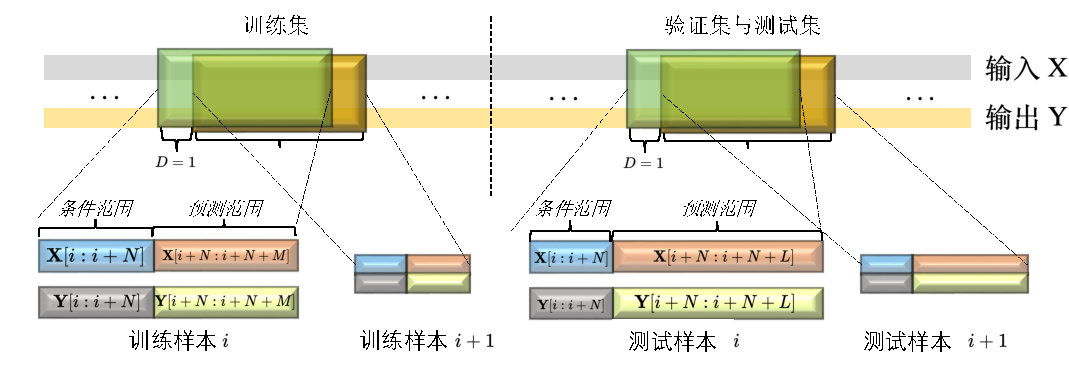
\includegraphics[width=\linewidth]{figures/chapter3/dataset.pdf}
    \caption{
    % Training set is built by moving a sliding window with speed $2$. Validation set and test set are built by moving a sliding window with speed $N+L$. $N$ is the length of encoded historical sequence. M is the length of predicted sequence in training phase. L is the length of predicted sequence in test or validation phase and it is a variable in different experiments.
    训练集、验证集、测试集的构建过程图示
    }
    \label{fig:dataset}
%\vspace*{-0.4cm}
\end{figure}


构造数据集的详细过程如图~\ref{fig:dataset}所示。
训练时,历史序列的长度为$N=80$,预测序列长度为$M=60$。
测试环节探究了$L=60, 200, 500$三种情况下,模型的预测性能。
模型仅利用训练集进行训练,验证集上表现最好的模型将被保留,并评估其在三个测试集上的表现。
% 然后使用不同的$L$生成不同的验证集和测试集,在其上进行验证和评估。
根据图~\ref{fig:dataset}所示的构建输入-输出序列对的方法,共计17,131个样本用于训练。对于不同预测长度$L=60、200、500$,分别有3561、3421、3121个样本用于测试。
所有的数据在训练和测试之前均被归一化为标准正态分布。

\subsection{实验参数及评价指标}

实验中,使用mini-batch随机梯度下降(SGD)和Adam优化器\cite{kingma2014adam}对模型进行训练。
批大小为$512$,初始学习率为$0.001$且按衰减率$0.95$指数衰减。衰减周期为10个训练轮次。
ODE-Net中隐藏状态$\b h(t)$的大小为$32$。
RNN序列编码器模块包含一个隐藏层,隐状态大小等于$32$(与$\boldsymbol h(t)$大小一致)。
状态解码器中隐藏层的大小为$64$。
% 训练时,找到在验证集上预测精度最高的模型,将其用于测试数据集精度评估。
训练和测试均在单个Nvidia V100 GPU上进行。
代码基于PyTorch框架实现。
对于给定的离散整数下标序列$[0,1,\dots, M]$, 我们定义其连续时间区间为 $0\leq t\leq M\delta_t$.
相邻数据点的时间间隔$\delta _t$被设置为0.1。
因此,式\eqref{equ:stationary}中的归一化因子$\mu _t$也被设置为0.1。
当使用欧拉数值求解器求解稳定系统的ODE方程时,模型将等价于直接使用GRU网络在离散时间系统下进行预测:
% \begin{equation}
\begin{align}
    \b h(t+\delta _t) &=\b h(t) + \delta _t \cdot \frac{\text{GRU}\big(\b h(t),x(t), \theta_d \big) - \b h(t)}{\mu _t}  \nonumber\\
                      &= \text{GRU}\big(\b h(t),x(t), \theta _d\big).
\end{align}
% \end{equation}

本节使用预测底流浓度的平均根相对平方误差(RRSE)和平均平方误差(MSE)评价不同模型的预测精度。RRSE是被归一化的均方根(RMS)误差。对于预测长度$L$,RRSE定义如下:
\begin{equation}
\begin{aligned}
    \text{RRSE}=\sqrt{\sum_{j=1}^{L} \frac{e_{j}^{2}}{\left(\hat{y}_{j}-\bar{y}\right)^{2}}}, \quad e_{j}=\hat{y}_{j}-y_{j}.
\end{aligned}
\label{equ:rrse}
\end{equation}


% \subsection{实验结果分析与讨论}

% To demonstrate the significance of proposed continuous-time system identification model.
% We construct two kinds of competitive baselines for substituting derivative module:
% \begin{equation}
%     \label{equ:nodiff_rnn}
%     \boldsymbol{h}(i+1)=R(\boldsymbol{h}(i), \boldsymbol{x}(i))
% \end{equation}
% \begin{equation}
%     \label{equ:diff_rnn}
%     \boldsymbol{h}(i+1)=R(\boldsymbol{h}(i), \boldsymbol{x}(i)) + \epsilon \boldsymbol{h}(i)
% \end{equation}
% Model with structure \eqref{equ:nodiff_rnn} is basic recurrent neural networks model which can be used to learn time series model and stationary system.

\subsection{不同模型预测结果对比}
首先,本节研究了不同ODE求解器和导数模块对预测精度的影响。
对比的ODE求解器包括五种:欧拉法(Euler)、中值法(Midpoint)、四阶龙格库塔(Runge—Kutta,RK4)、 Dormand—Prince(Dopri5)\cite{NIPS2018_7892}、以及三阶Bogacki—Shampine(Bosh)\cite{bogacki19893}。
% 微分方程求解器在设定自适应微分方程求解器参数时,由于降低近似误差的容忍度,会导致求解常微分方程的时间剧烈增加。
为了平衡时间消耗和预测精度,本节将所有自适应求解器的相对误差限设置为$1\mathrm{e}-4$,绝对误差限设置为$1\mathrm{e}-5$。
本节研究了上述微分方程求解器在非稳定和稳定系统两种情况下的求解性能。
此外,我们还评估了部分离散时间深度序列模型的预测效果,包括深度状态空间模型(DT-State-Space)、基于注意力机制的Seq2Seq模型(Attention-Seq2Seq)\cite{Member2019}和Transformer模型\cite{Wu2020}。
DT-State-Space~\cite{Rangapuram2018}模型采用循环神经网络(RNN)建模线性状态空间模型的动态参数,并利用预测得到的状态空间模型预测时间序列,其状态空间和RNN隐藏层的大小分别设置为16和32。
Transformer和Attention-Seq2Seq的超参数设置与原文献保持一致。

% Table~\ref{tab:3_exp_all} presents the results of the predicted underflow concentrations. 
\begin{table*}[htpb]
%\setlength{\abovecaptionskip}{-0.1cm} 
\caption{
%%%%%%%
% seeking help : 预测底流浓度的RRSE、MSE 误差 以及每次预测序列所需的时间
%RRSE and MSE error of predicted underflow concentration and time consumption for each prediction.
底流浓度预测的相对方根误差(RRSE)、平均平方误差(MSE)、时间消耗
% Root relative squared error (RRSE), mean squared error (MSE), and time consumption of predicted underflow concentration.
}
%%%%%%%
\label{tab:3_exp_all}
\centering
% \setlength{\tabcolsep}{3.0mm}{%7可随机设置,调整到适合自己的大小为止
\resizebox{\linewidth}{!}{
\footnotesize
% \renewcommand{\arraystretch}{1.5}
\begin{tabular}{c|c|ccccccccc}
\toprule
\multicolumn{2}{c|}{\multirow{2}{*}{模型}}                                                                        & \multicolumn{3}{c|}{$L=60$}                                                           & \multicolumn{3}{c|}{$L=200$}                                                           & \multicolumn{3}{c}{$L=500$}                                         \\ \cline{3-11} 
\multicolumn{2}{c|}{}                                                                                              & RRSE                 & MSE                  & \multicolumn{1}{c|}{时间(s)}             & RRSE                 & MSE                  & \multicolumn{1}{c|}{时间(s)}              & RRSE                 & MSE                  & 时间 (s)                \\ \hline
\multirow{4}{*}{\begin{tabular}[c]{@{}c@{}}非稳定\\ 系统\end{tabular}} & \multicolumn{1}{c|}{Euler}     & 3.18                 & 9.07                 & \multicolumn{1}{c|}{1.71}             & 5.09                 & 80.25                & \multicolumn{1}{c|}{3.81}              & 3.95                 & 152.21               & 4.65                 \\
                                                                                 & \multicolumn{1}{c|}{Mid-Point} & 3.10                 & 8.95                 & \multicolumn{1}{c|}{3.23}             & 5.24                 & 80.29                & \multicolumn{1}{c|}{7.36}              & 4.16                 & 172.43               & 9.15                 \\
                                                                                 & \multicolumn{1}{c|}{RK4}       & 3.10                 & 8.97                 & \multicolumn{1}{c|}{6.95}             & 5.24                 & 83.90                & \multicolumn{1}{c|}{14.82}             & 4.16                 & 172.64               & 18.76                \\
                                                                                 & \multicolumn{1}{c|}{Bosh}    & 3.08  & 8.57  & \multicolumn{1}{c|}{12.8}             & 5.84                 & 84.60                & \multicolumn{1}{c|}{19.0}              & 4.61                 & 172.39               & 24.75                \\
                                                                                 & \multicolumn{1}{c|}{Dopri5}    &  \uline{\textbf{2.83}}  &  \uline{\textbf{6.40}}  & \multicolumn{1}{c|}{9.63}             & 5.31                 & 84.60                & \multicolumn{1}{c|}{13.8}              & 4.19                 & 175.39               & 25.75                \\ \hline
\multirow{4}{*}{\begin{tabular}[c]{@{}c@{}}稳定\\ 系统\end{tabular}}     & \multicolumn{1}{c|}{Euler}     & 3.18                 & 9.06                 & \multicolumn{1}{c|}{1.63}             & 3.75                 & 34.78                & \multicolumn{1}{c|}{3.58}              & 1.63                 & 37.77                & 4.66                 \\
                                                                                 & \multicolumn{1}{c|}{Mid-Point} & 3.18                 & 9.08                 & \multicolumn{1}{c|}{3.22}             & 3.73                 & 34.64                & \multicolumn{1}{c|}{7.17}              & 1.62                 & 38.36                & 9.3                  \\
                                                                                 & \multicolumn{1}{c|}{RK4}       & 3.18                 & 8.96                 & \multicolumn{1}{c|}{6.80}             &  \uline{\textbf{3.58}}  &  \uline{\textbf{32.90}} & \multicolumn{1}{c|}{15.17}             &  \uline{\textbf{1.61}}  &  \uline{\textbf{34.88}} & 18.66                \\
                                                                                 & \multicolumn{1}{c|}{Bosh}    & N/A                    & N/A                    & \multicolumn{1}{c|}{\textgreater{}50} & N/A                    & N/A                    & \multicolumn{1}{c|}{\textgreater{}200} & N/A                    & N/A                    & \textgreater{}3000   \\
                                                                                 & \multicolumn{1}{c|}{Dopri5}    & N/A                    & N/A                    & \multicolumn{1}{c|}{\textgreater{}50} & N/A                    & N/A                    & \multicolumn{1}{c|}{\textgreater{}200} & N/A                    & N/A                    & \textgreater{}3000   \\ \hline
\multicolumn{2}{c|}{Attention-Seq2Seq\cite{Member2019}}                                                                             & 3.13                 & 8.97                 & \multicolumn{1}{c|}{0.41}             & 4.02                 & 33.90                & \multicolumn{1}{c|}{0.41}              & 1.82                 & 40.53                & 0.42                 \\ \hline
\multicolumn{2}{c|}{DT-State-Space\cite{Rangapuram2018}}                                                                               & 3.22                 & 9.36                 & \multicolumn{1}{c|}{0.06}             & 4.69                 & 41.11                & \multicolumn{1}{c|}{0.07}              & 3.35                 & 45.64                & 0.08                 \\
\multicolumn{2}{c|}{Transformer\cite{Wu2020}}                                                                               & 3.16                 & 8.36                 & \multicolumn{1}{c|}{0.02}             & 3.99                 & 40.23                & \multicolumn{1}{c|}{0.02}              & 2.55                 & 44.23                & 0.03                 \\
\bottomrule
\end{tabular}}
\end{table*}

本节共进行了三组实验以探究不同预测长度$L=60$、$200$和$500$下,不同模型预测结果的RRSE、MSE和预测时间。
从表~\ref{tab:3_exp_all}可以发现,离散时间域下的Attention-Seq2Seq模型、DT-State-Space模型和Transformer的性能稍优于使用Euler求解器时的预测效果,但差于使用高阶ODE求解器的预测效果,特别是在长期预测$L=200, 500$时表现更为明显。
结果表明,采用连续时间模型可以更好地反映浓密机系统的连续时间演化特征,从而相比于离散时间模型具有更高的预测精度。

\subsection{不同ODE求解器下稳定系统以及非稳定系统对比}
表~\ref{tab:3_exp_all}分别评估了稳定系统模型和非稳定系统模型在不同ODE求解器下的预测误差。

当导数模块为非稳定系统时,对于短期预测任务($L = 60$),
虽然Euler求解器的时间消耗低于其他ODE求解器,但其预测结果的RRSE和MSE较高,预测精度差于其他四个ODE求解器。
原因在于欧拉方法作为求解ODE方程最简单的方法,它在两个相邻时间点之间仅调用一次导数模块以计算隐状态的单步差分。
其运行本质等同于离散时间序列模型,因为并没有充分利用模型为连续时间系统的性质,所得ODE方程的解的精度较差。
相应地,中值法和4阶龙格库塔法在两个相邻时间点之间分别调用了导数模块两次和四次。因此,这两种方法对隐状态轨迹的求解精度高于欧拉法,预测精度优于基于Euler方法的离散时间模型。


另外,
% 作为隶属于龙格-库塔体系中的常微分方程自适应步长求解方法,Dopri5和Bosh方法
Dopri5和Bosh方法作为自适应步长的求解器,
能够确保数值解与真实解之间的误差限定在指定误差范围内。
随着给定误差限的缩小,求解ODE方程的时间消耗也随之增加。
虽然两种方法求解ODE的耗时较长,但精度较高。Dopri5的预测性能稍好于Bosh。

%It is also equivalent to standard discrete-time deep sequential model which is the most common choice for formulating an evenly sampled dynamical system.

% 当导数模块分别被定义为非稳定系统与稳定系统时,ODE求解器在预测精度和时间消耗上表现也会收到
% 实验中,我们还发现,同一ODE求解器在预测精度和时间消耗上表现也会受到导数模块定义的影响。
当导数模块定义为平稳系统时。
两种自适应方法Bosh和Dopri5求解ODE方程的时间消耗将显著增加。
在表\ref{tab:3_exp_all}中,我们没有列出Dopri5和Bosh在稳定系统中的预测精度,因为其计算速度极慢,无法在限定时间内给出ODE的解。
求解ODE所需的时间会大幅增加,其原因是相比于非稳定系统,稳定系统会使得隐状态的轨迹波动更加剧烈。
本质上,稳定系统中的$\text{GRU}\left(\mathbf{h}(t), \mathbf{x}(t), \theta_{d}\right)$根据$\b h^{\infty}(t)$定义了目标状态$\b h^{\infty}(t)$,满足$\text{GRU}\left(\mathbf{h}^{\infty}(t), \mathbf{x}(t), \theta_{d}\right)=\mathbf{h}^{\infty}(t)$。
隐状态沿着方向$\overrightarrow{\mathbf{h}^\infty-\mathbf h(t)}$向目标状态移动。
由于数据集中外部输入$\b x(t)$是持续变化且不稳定的,因此会导致$\b h^{\infty}(t)$剧烈变化。
% When the ODE equation is solved numerically with other ODE solvers whose orders are constant, such as Euler or Mid-point method, the number of times for evaluating derivative module is constant and the step size $\Delta t$ is not short enough to estimate the system trajectory accurately under unstable $\b x(t)$.
当采用Euler、rk4等导数访问次数固定的求解器时,使用固定步长$\Delta t$无法在$\b x(t)$持续变化的情况下精确地求解系统轨迹。
% The adaptive Dopri5 method has to reduce the $\Delta t$ drastically to control the numerical error constrained in a given tolerance which leads to enormous time cost.
自适应步长求解器Dopri5、Bosh为了满足给定的误差限要求,不得不急剧减小$\Delta t$以求解精确的隐状态轨迹,因此使求解ODE所需的时间剧烈增加。

总体来看,高阶ODE求解器的求解误差小于低阶ODE求解器,但在求解ODE方程时需要消耗更多的时间。
虽然本章所提出的连续时间ODE-Net模型在预测精度上表现良好,但与其他模型相比,推理速度较慢。
表\ref{tab:3_exp_all}的最后一列表示预测序列长为$L$时,模型的平均消耗时间。
因为在ODE-Net的训练和推理中,其前向传播和反向传播过程都需要大量地计算隐状态导数。
因此在预测系统动态变化时,其时间消耗远高于离散时间模型。
一些前沿研究\cite{J2020,poli2020,kelly2020}聚焦于优化ODE-Net的训练或推理速度。
这些方法为提高本章模型的预测效率提供了有借鉴意义的指导。

% \subsection{稳定系统与非稳定系统对比}

为了更直观地比较稳定系统和非平稳系统在长短期预测时的区别,本节对预测结果进行了可视化分析。
图\ref{fig:predict_cmp_60}描述了在$L=60$的短期预测任务中,使用不同ODE求解器求解非平稳系统和平稳系统得到的预测序列:

\begin{figure}[htpb]
\centering
%\setlength{\abovecaptionskip}{-0.1cm} 
\subfigure[稳定系统+RK4求解器]{
\begin{minipage}[t]{\linewidth}
\centering
% \hspace{-22pt}
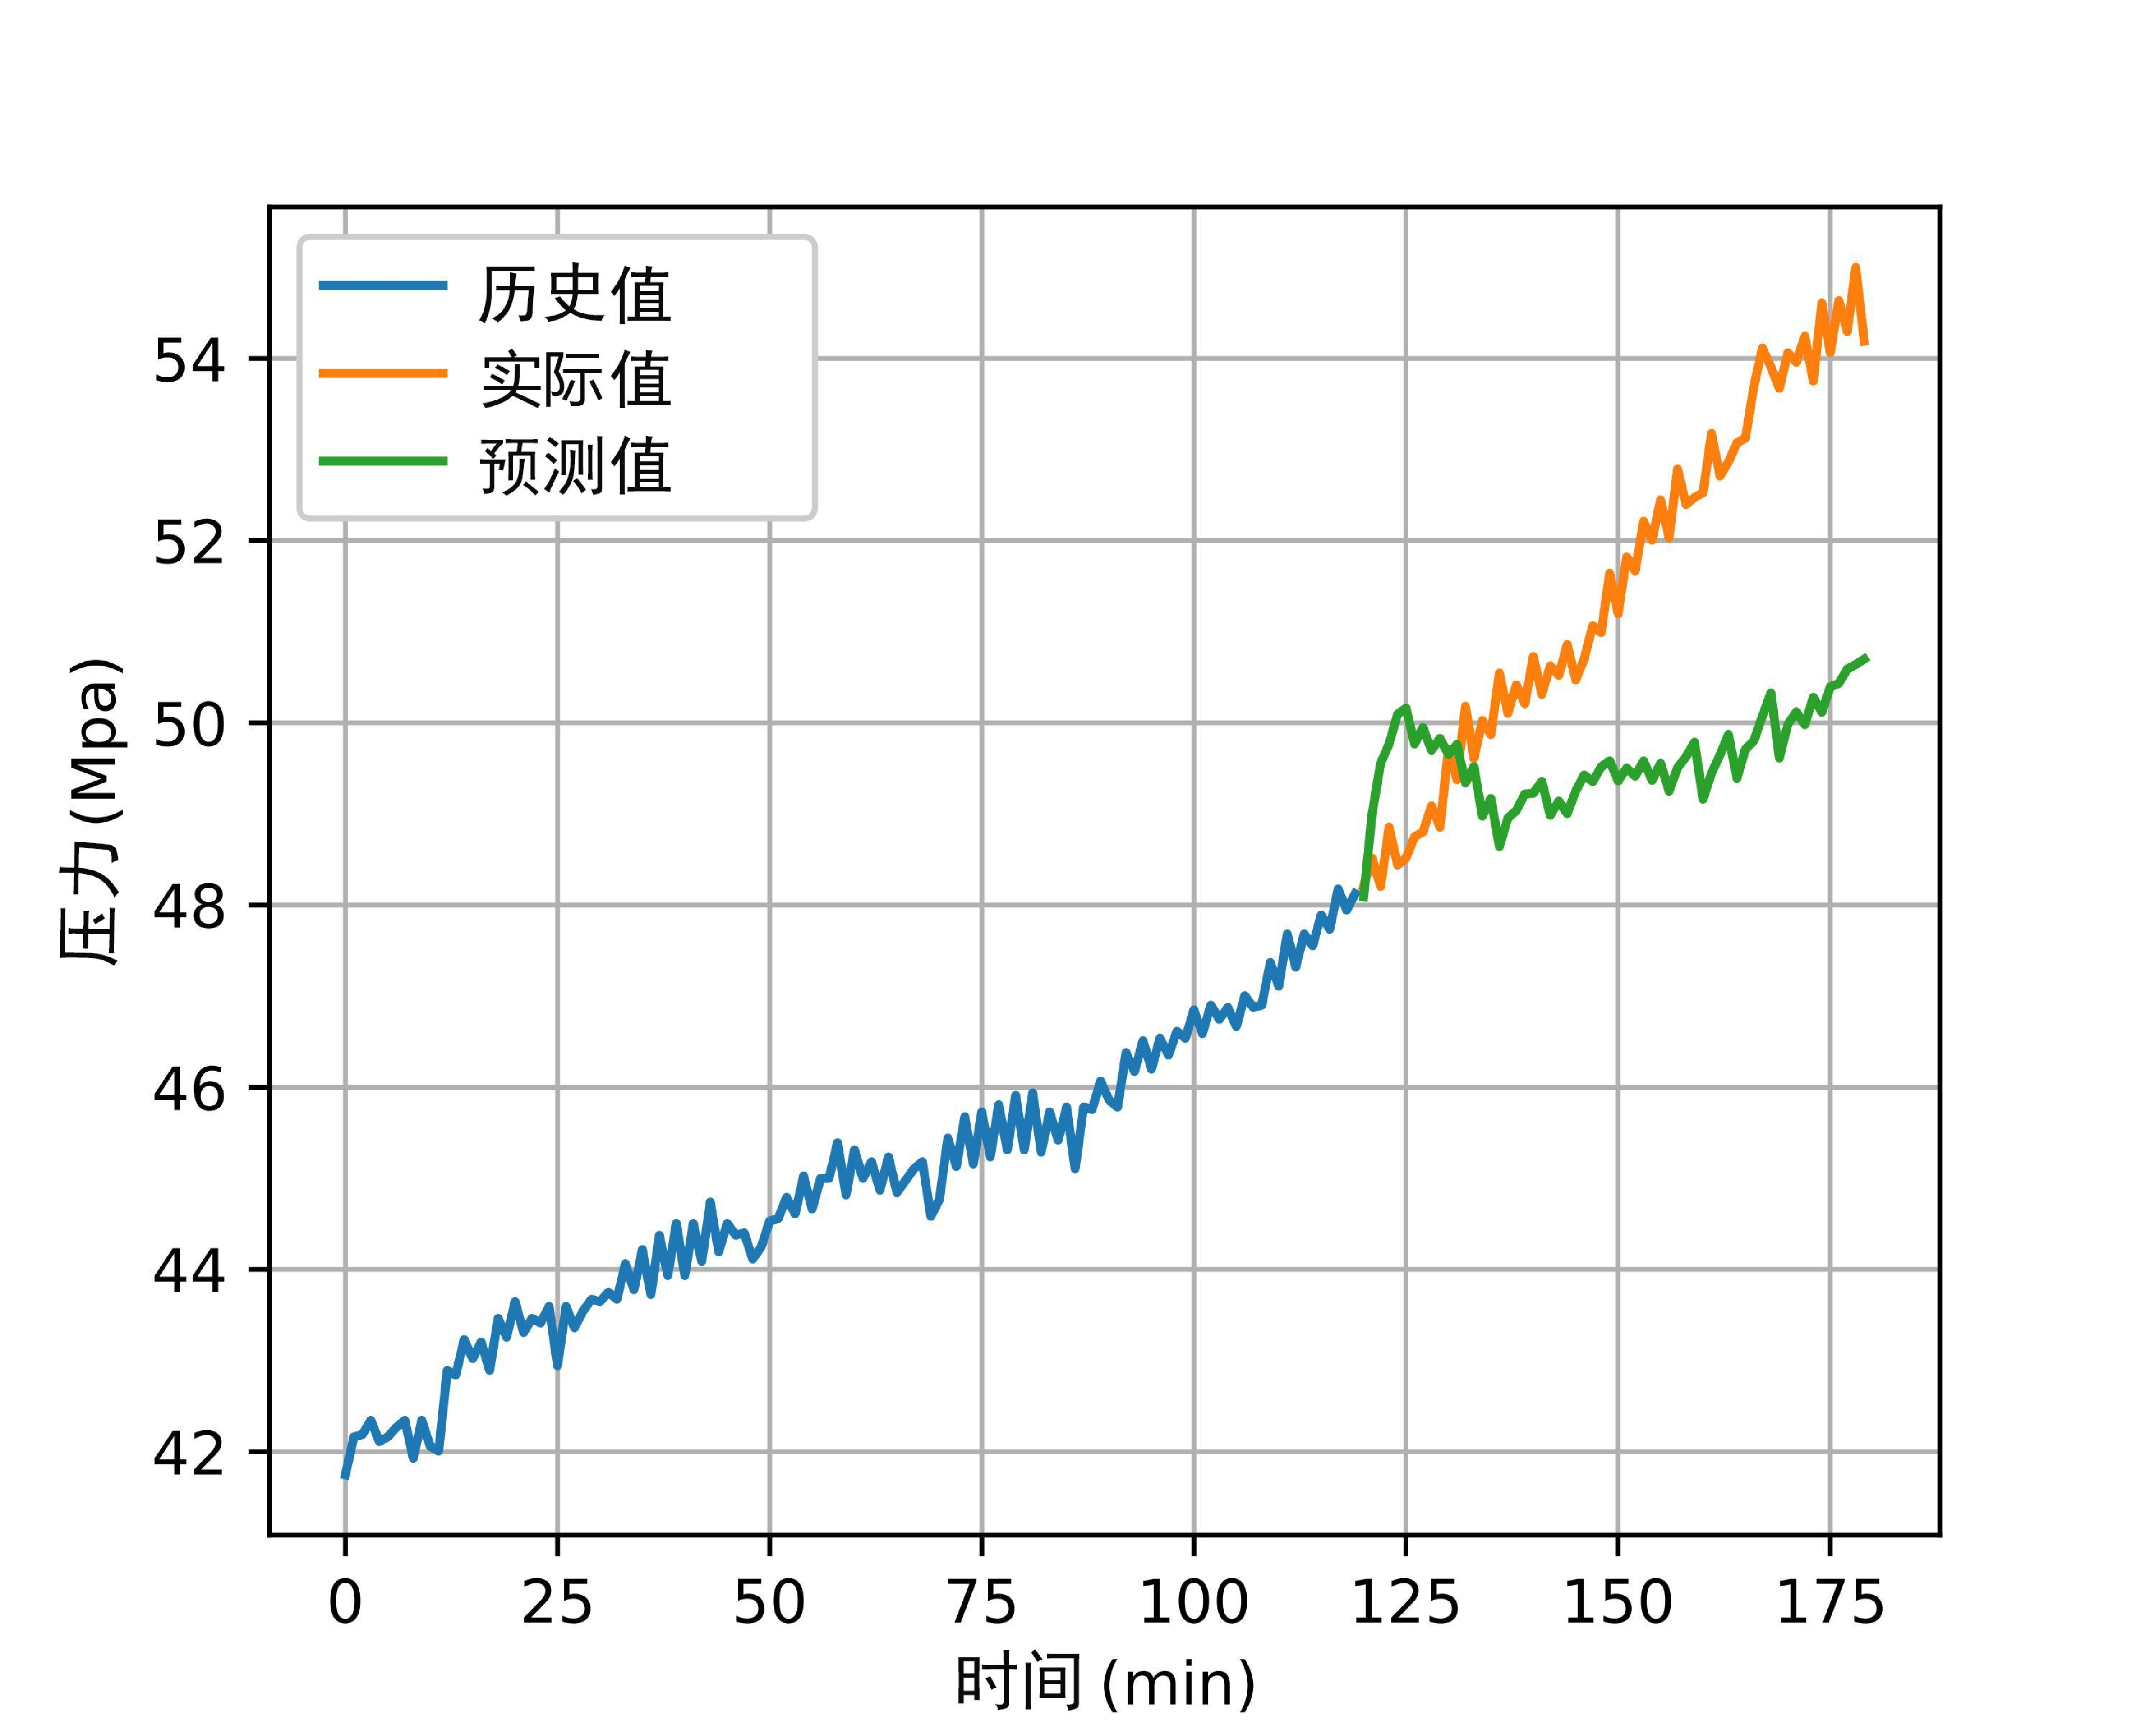
\includegraphics[width=0.49\linewidth,trim=50 0 0 200,clip]{figures/chapter3/predict_cmp/Pressure_GRU_sta_rk4_60.pdf}
% \hspace{-18pt}
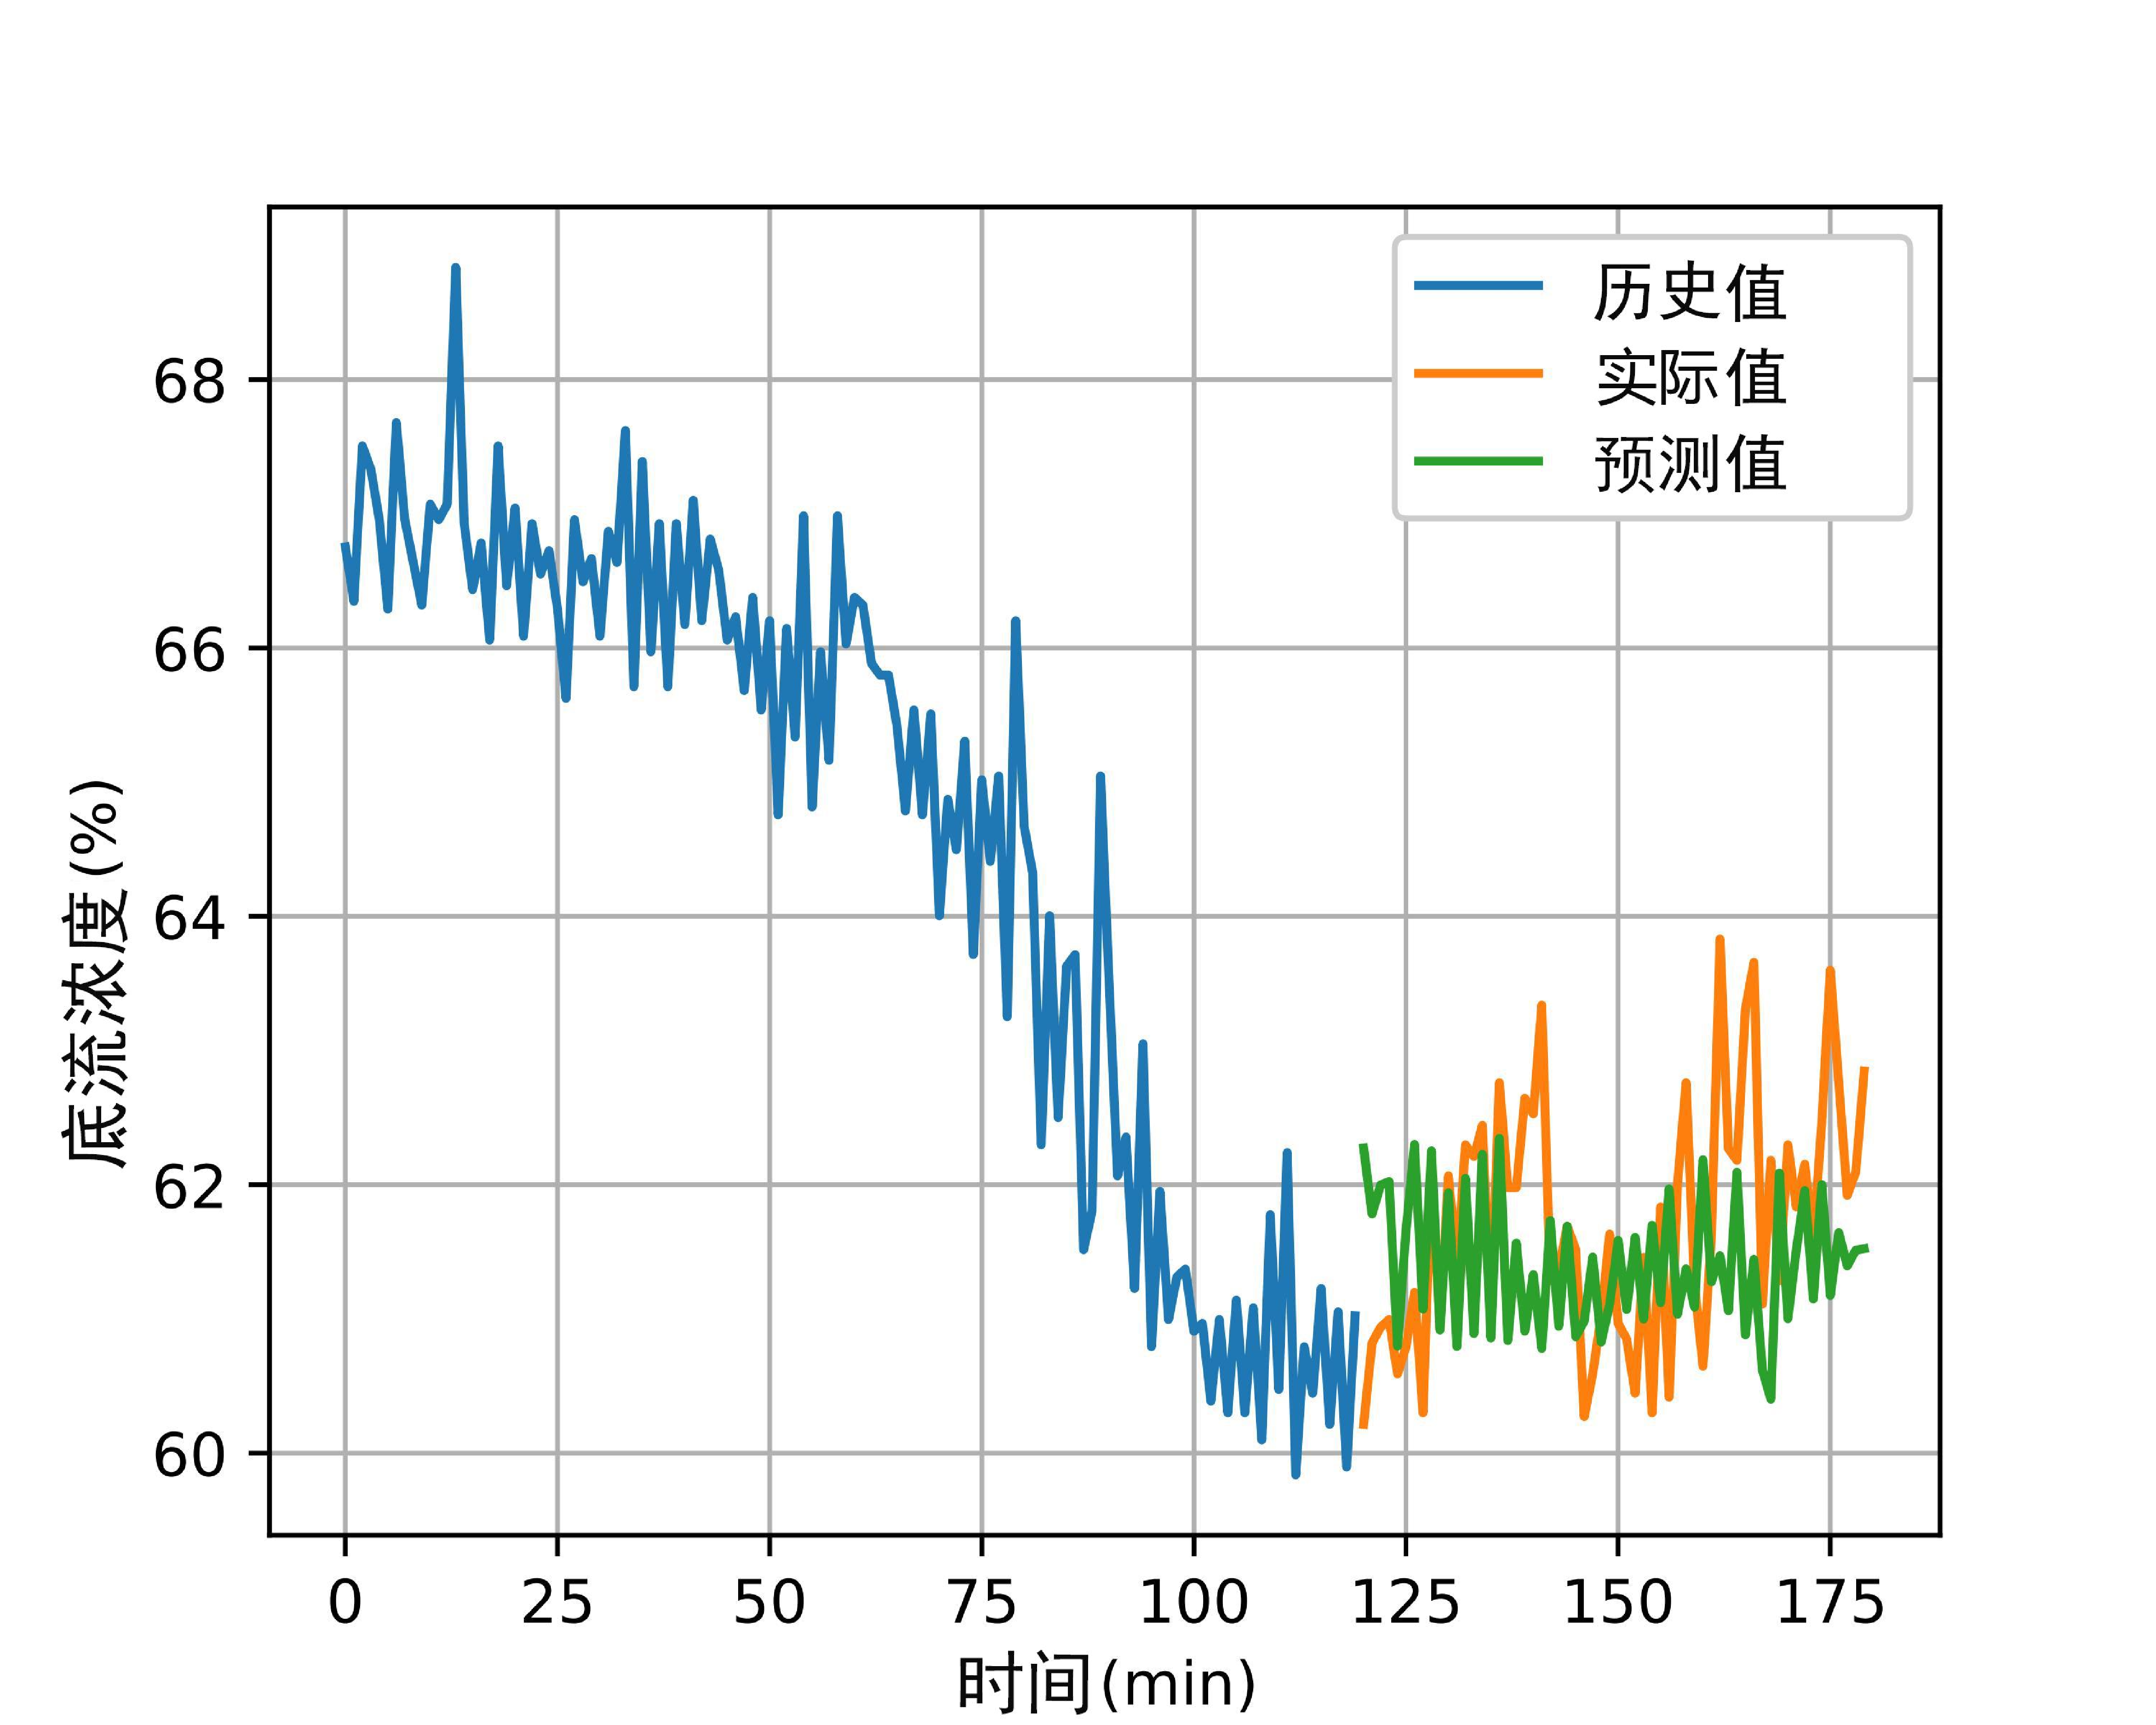
\includegraphics[width=0.49\linewidth,trim=50 0 0 200,clip]{figures/chapter3/predict_cmp/UC_GRU_sta_rk4_60.pdf}
%\caption{fig1}
\end{minipage}
}%

% \hspace{-22pt}
\subfigure[非稳定系统+RK4求解器]{
\begin{minipage}[t]{\linewidth}
\centering
% \hspace{-22pt}
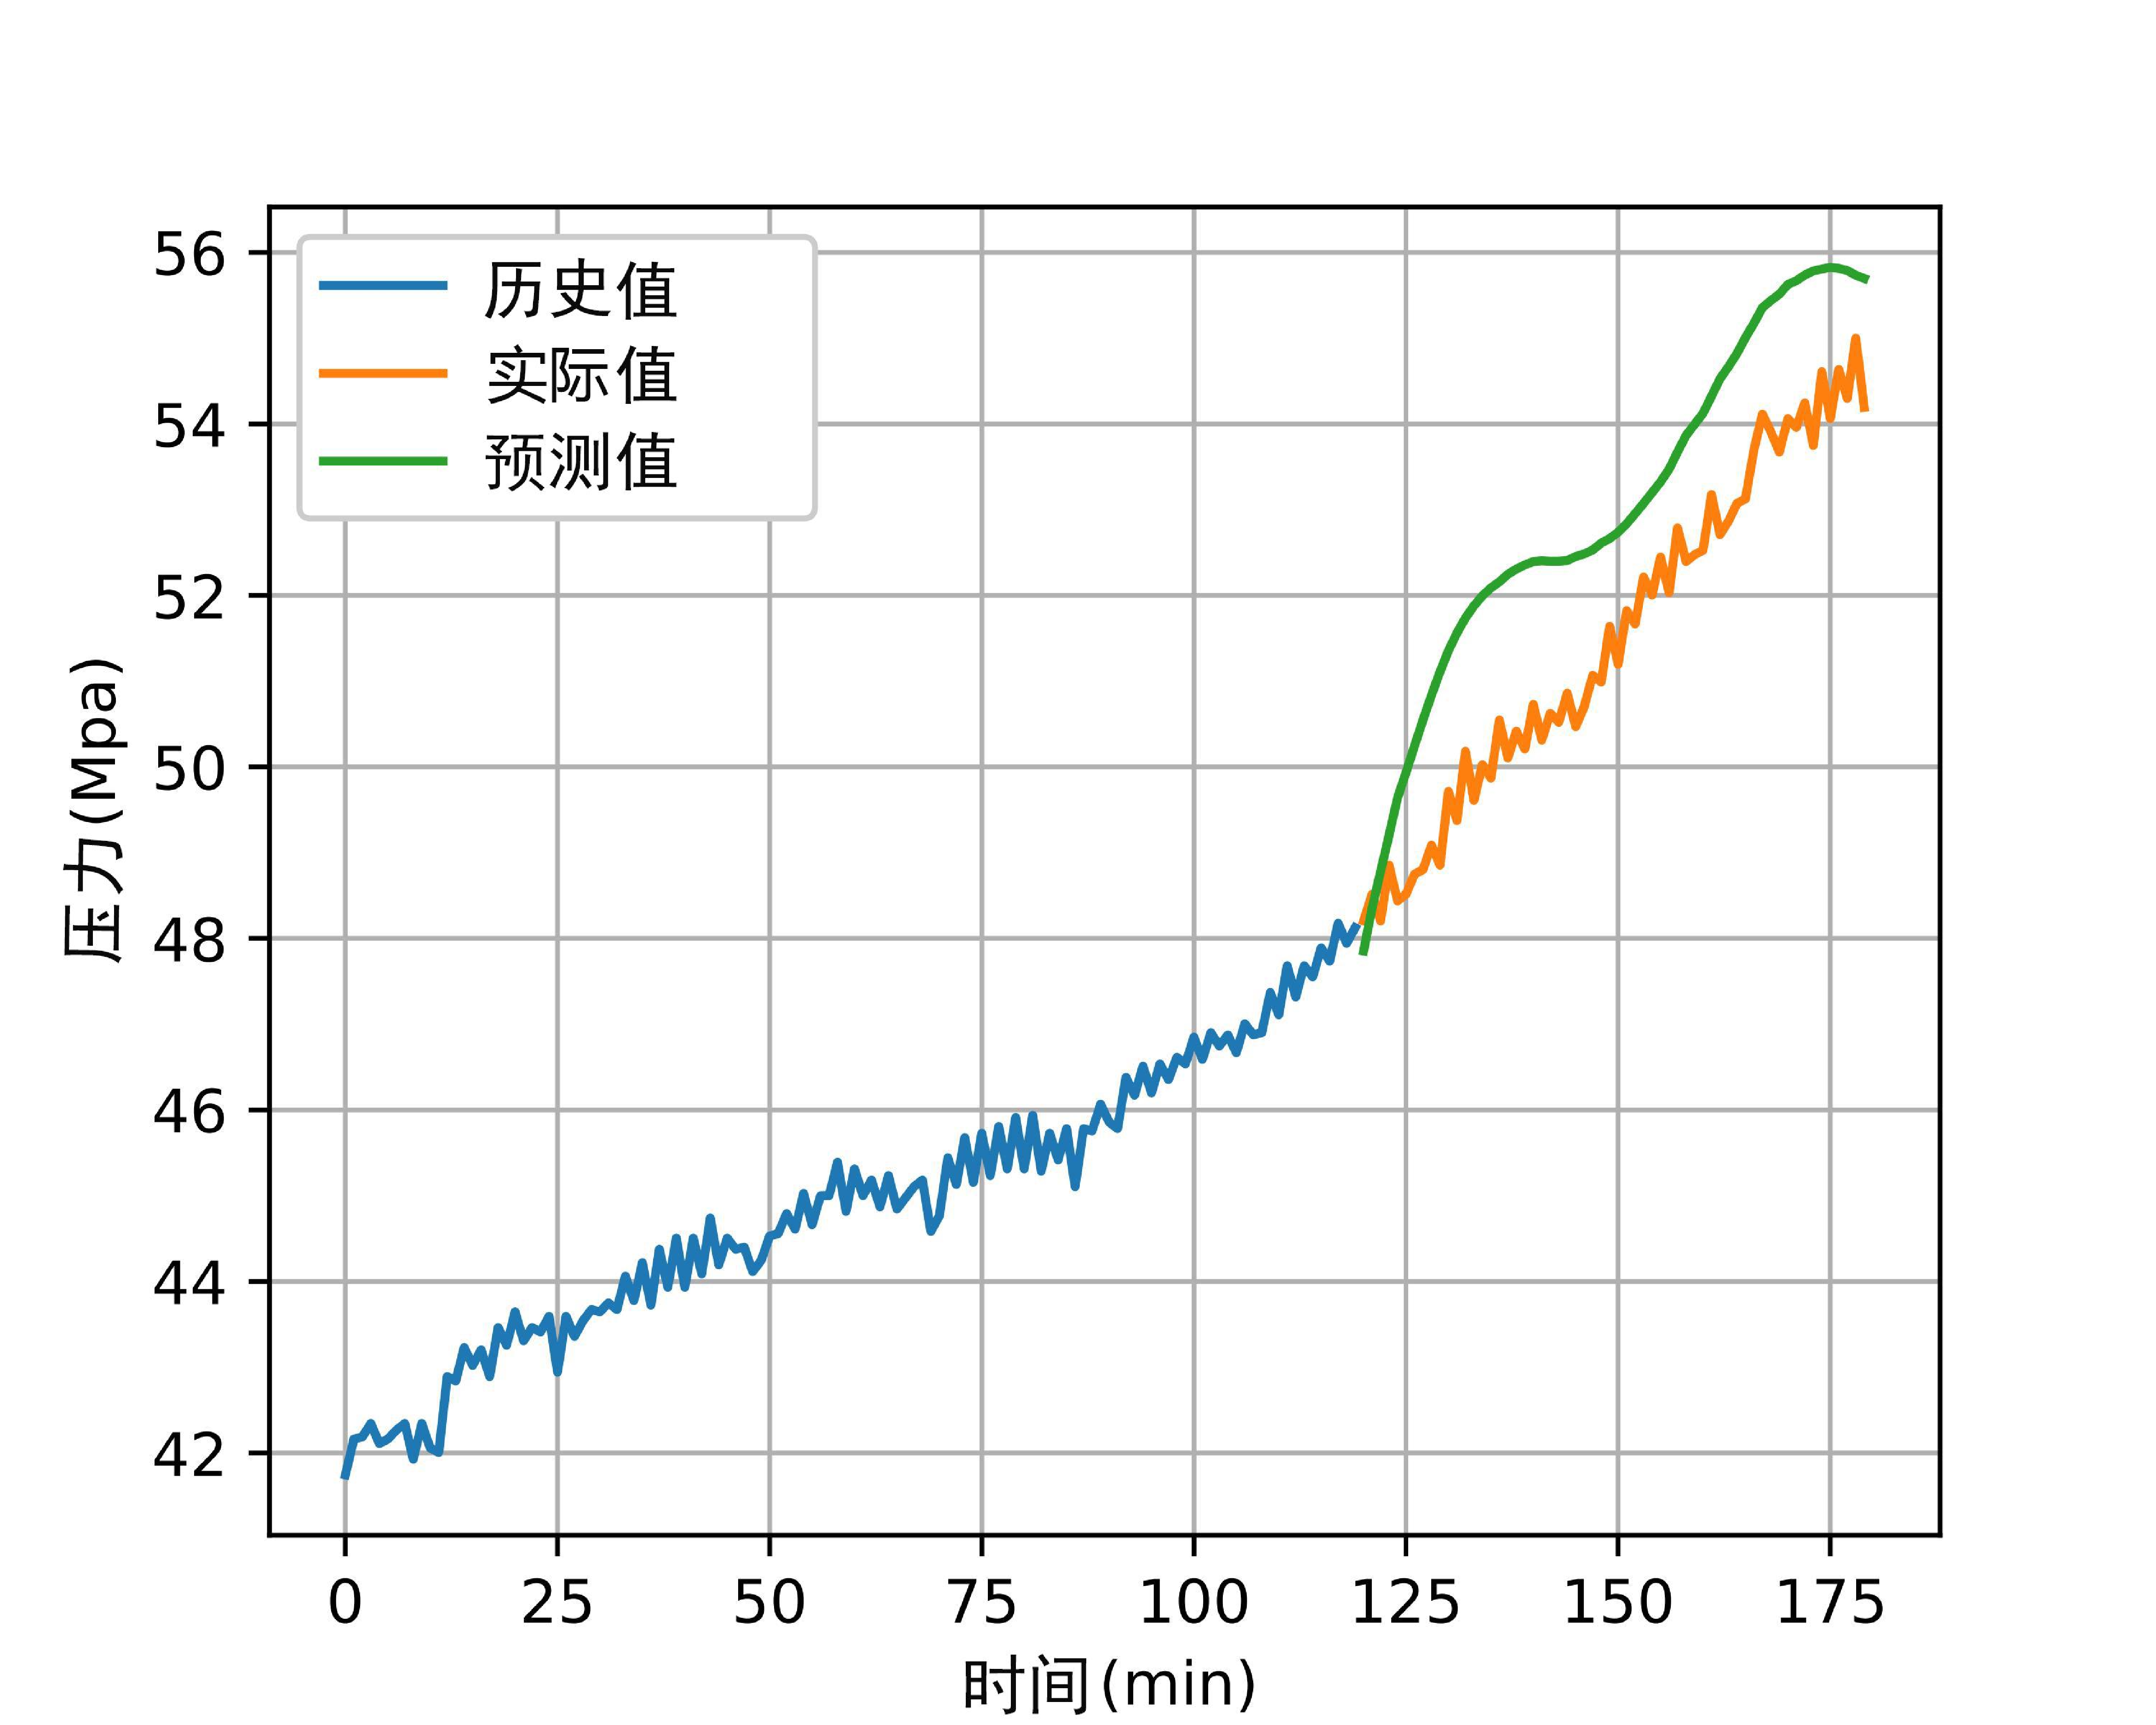
\includegraphics[width=0.49\linewidth,trim=50 0 0 200,clip]{figures/chapter3/predict_cmp/Pressure_MLP_nonsta_rk4_60.pdf}
% \hspace{-18pt}
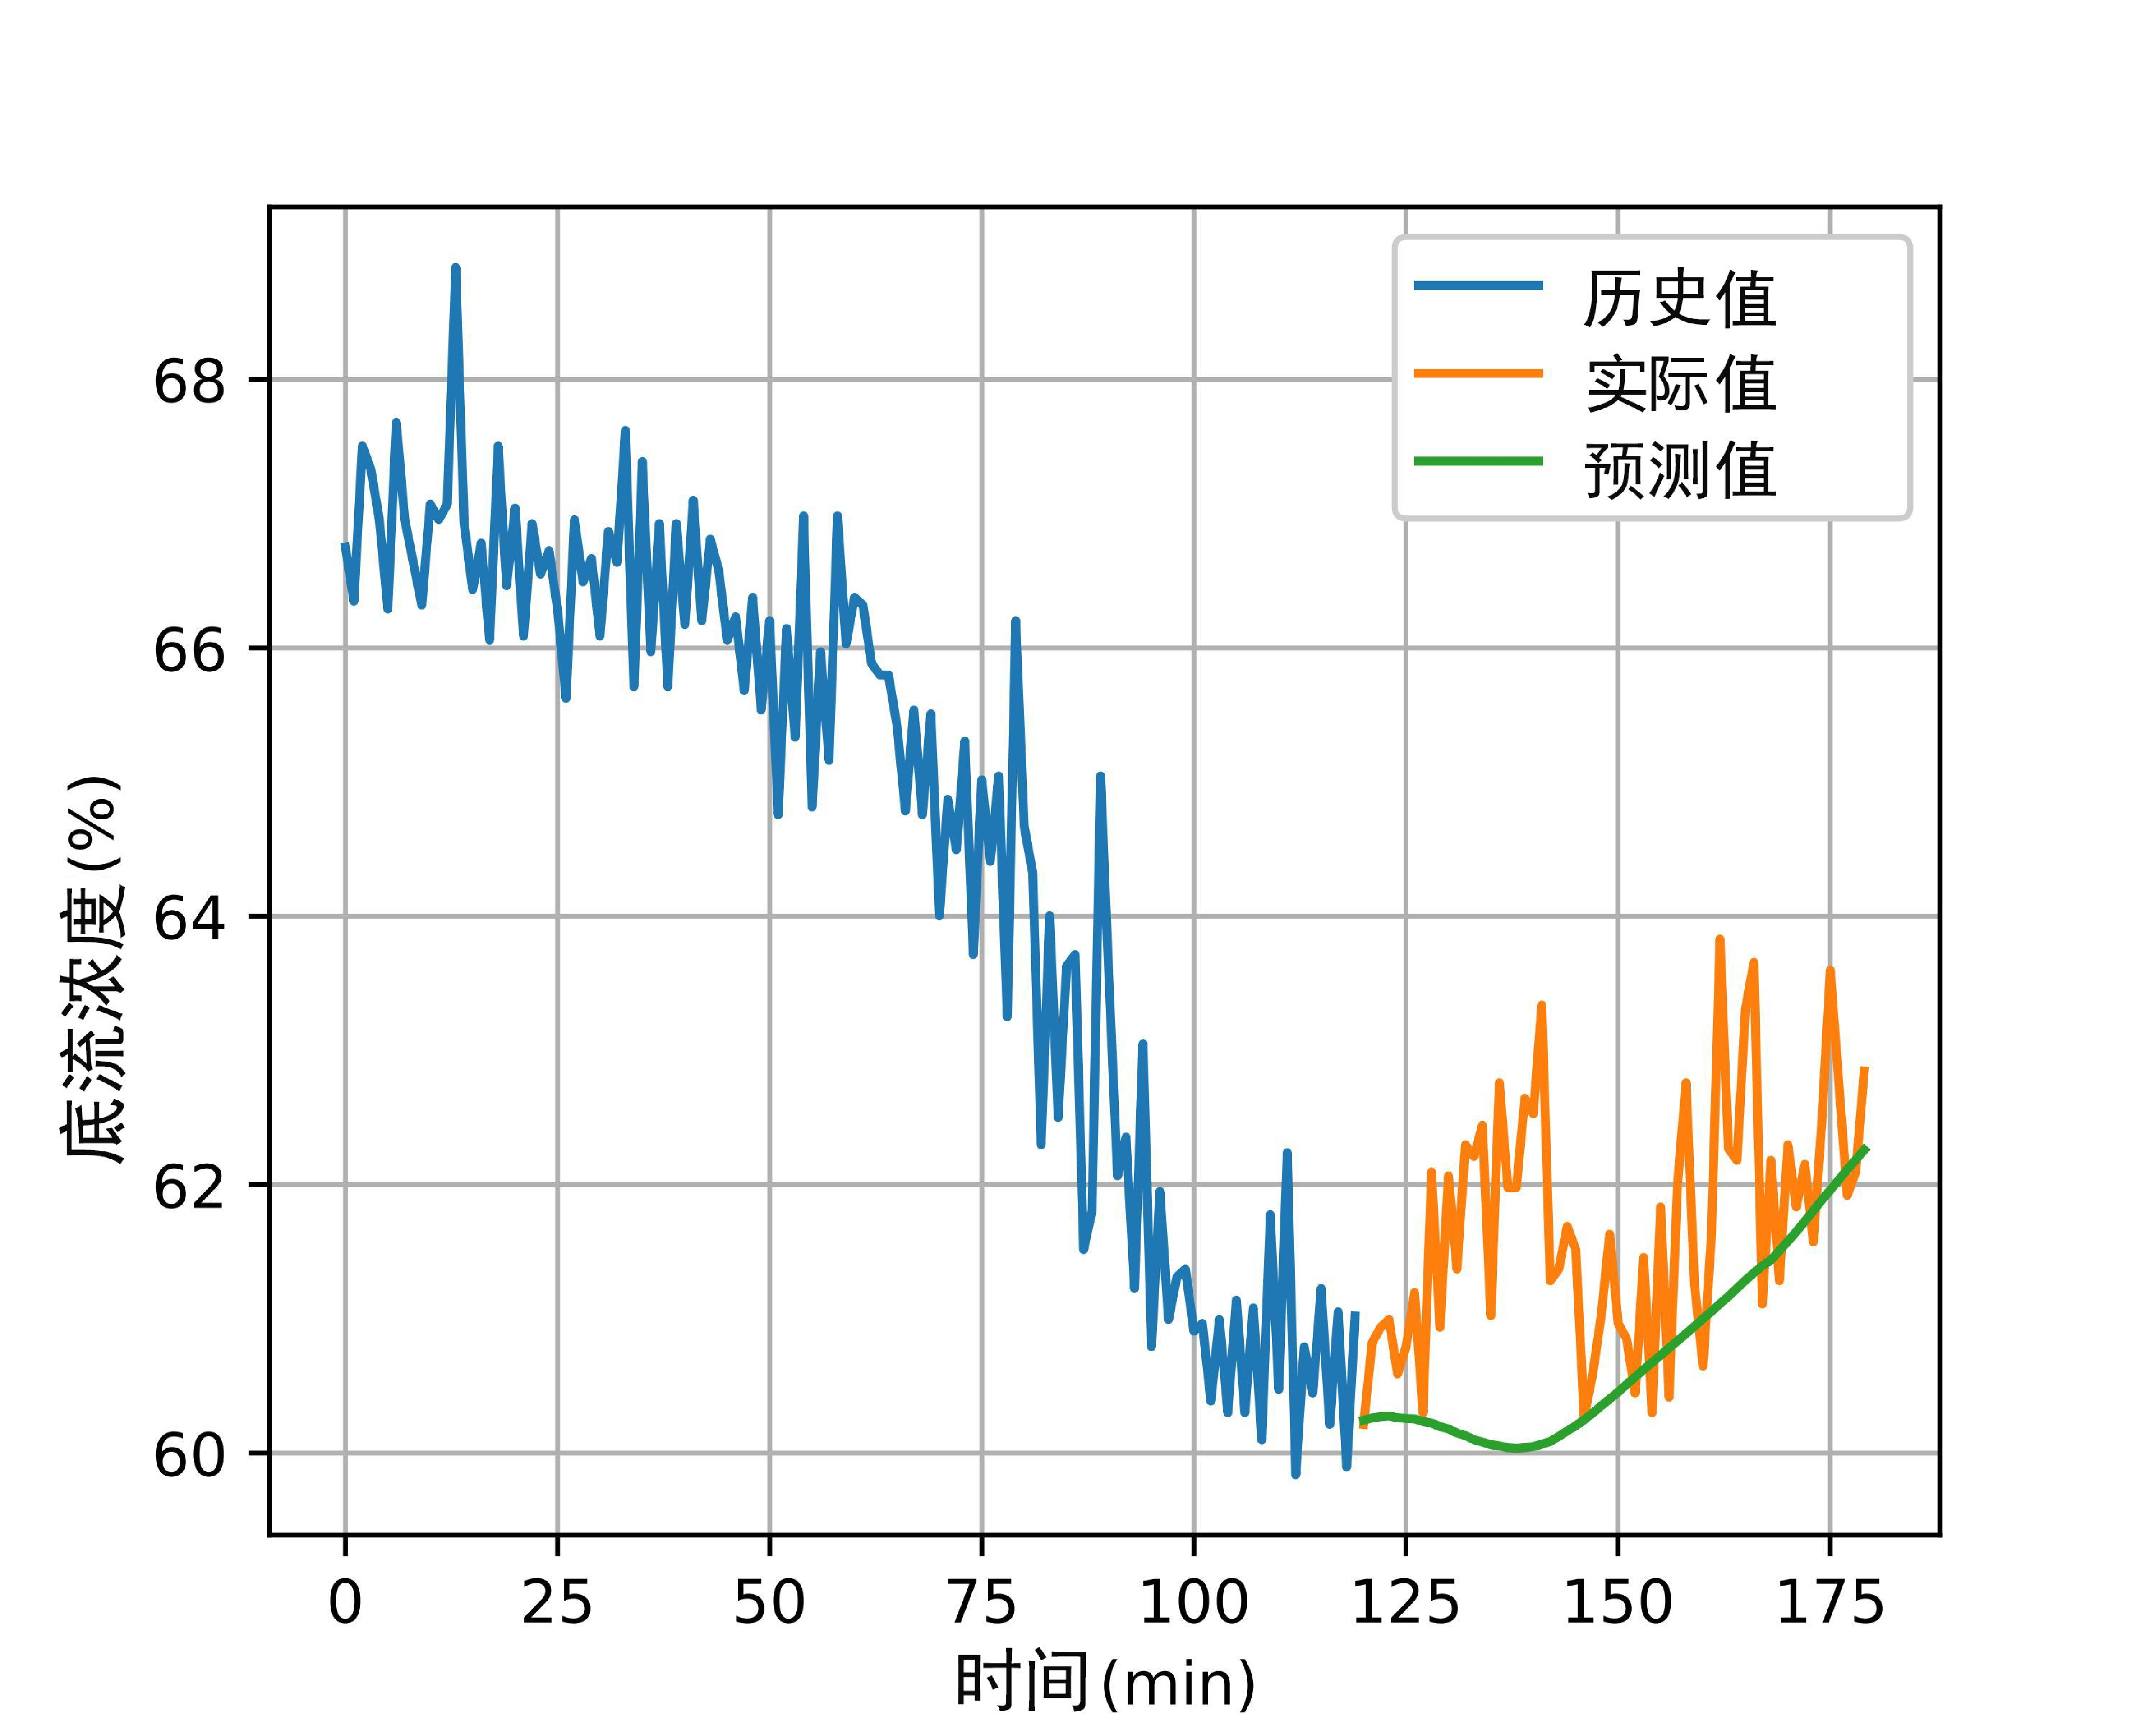
\includegraphics[width=0.49\linewidth,trim=50 0 0 200,clip]{figures/chapter3/predict_cmp/UC_MLP_nonsta_rk4_60.pdf}
%\caption{fig1}
\end{minipage}
}%

% \hspace{-22pt}
\subfigure[非稳定系统+Dopri5求解器]{
\begin{minipage}[t]{\linewidth}
\centering
% \hspace{-22pt}
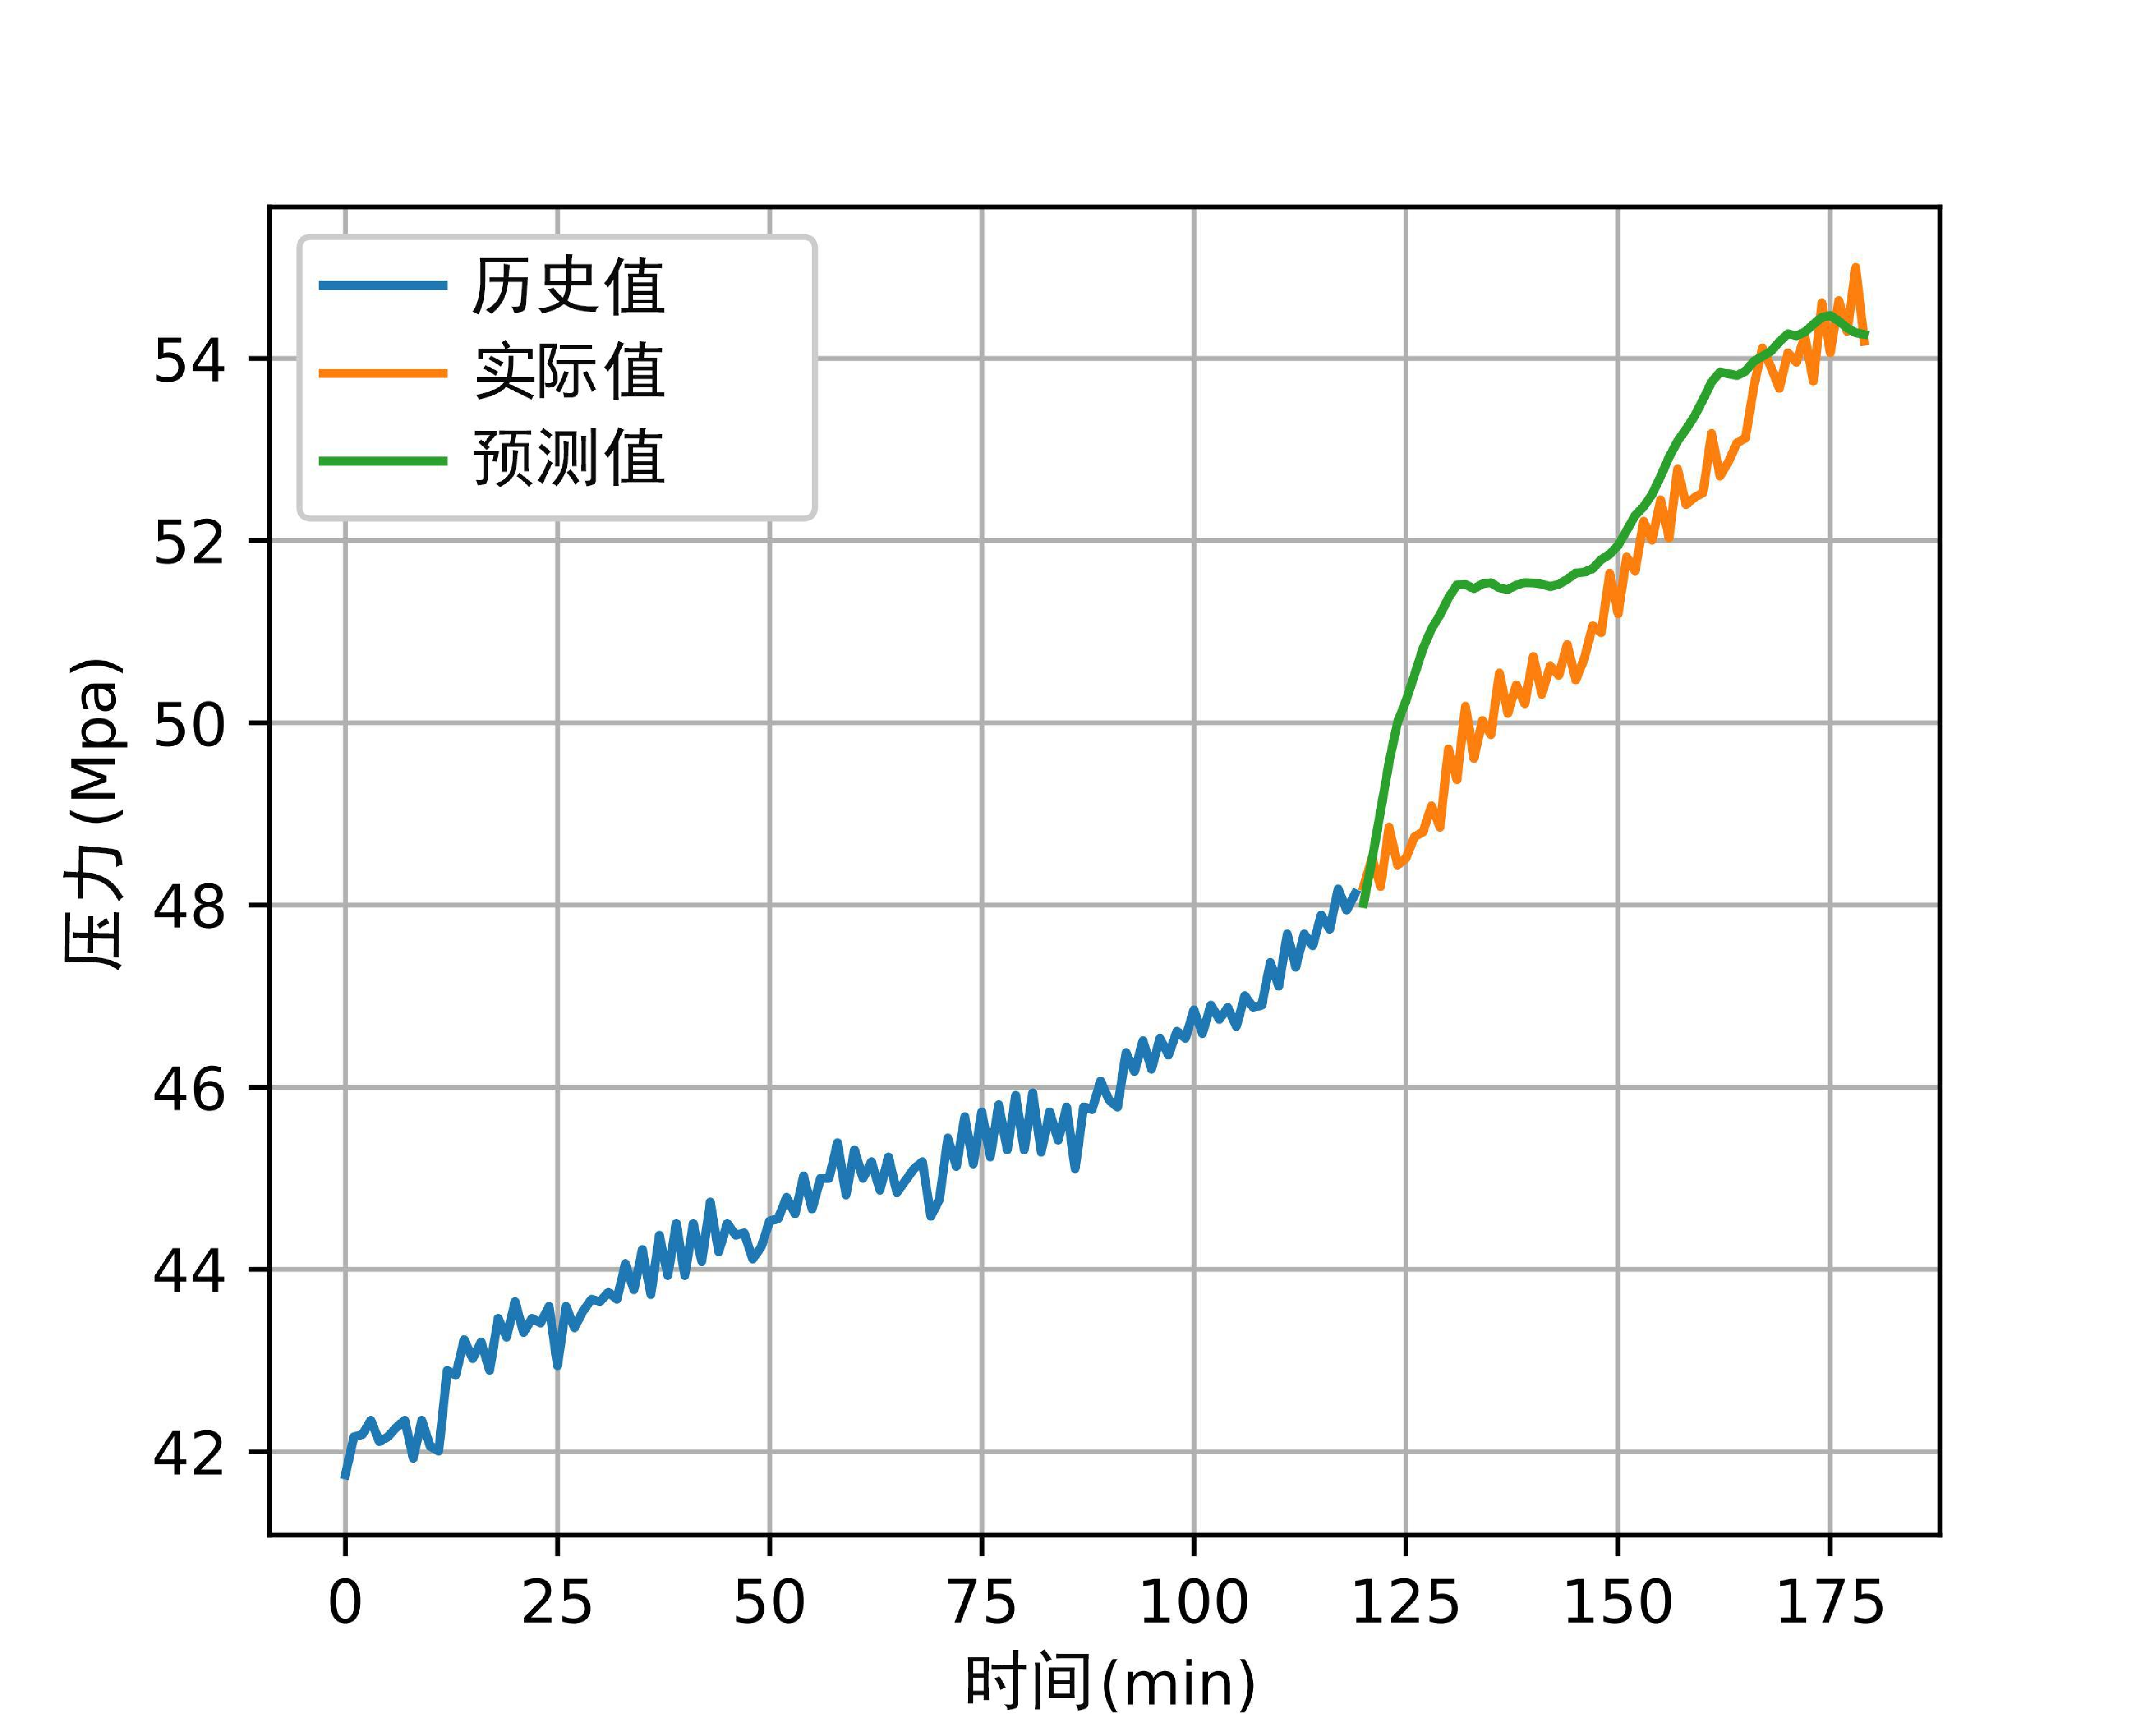
\includegraphics[width=0.49\linewidth,trim=50 0 0 200,clip]{figures/chapter3/predict_cmp/Pressure_MLP_nonsta_dopri5_60.pdf}
% \hspace{-18pt}
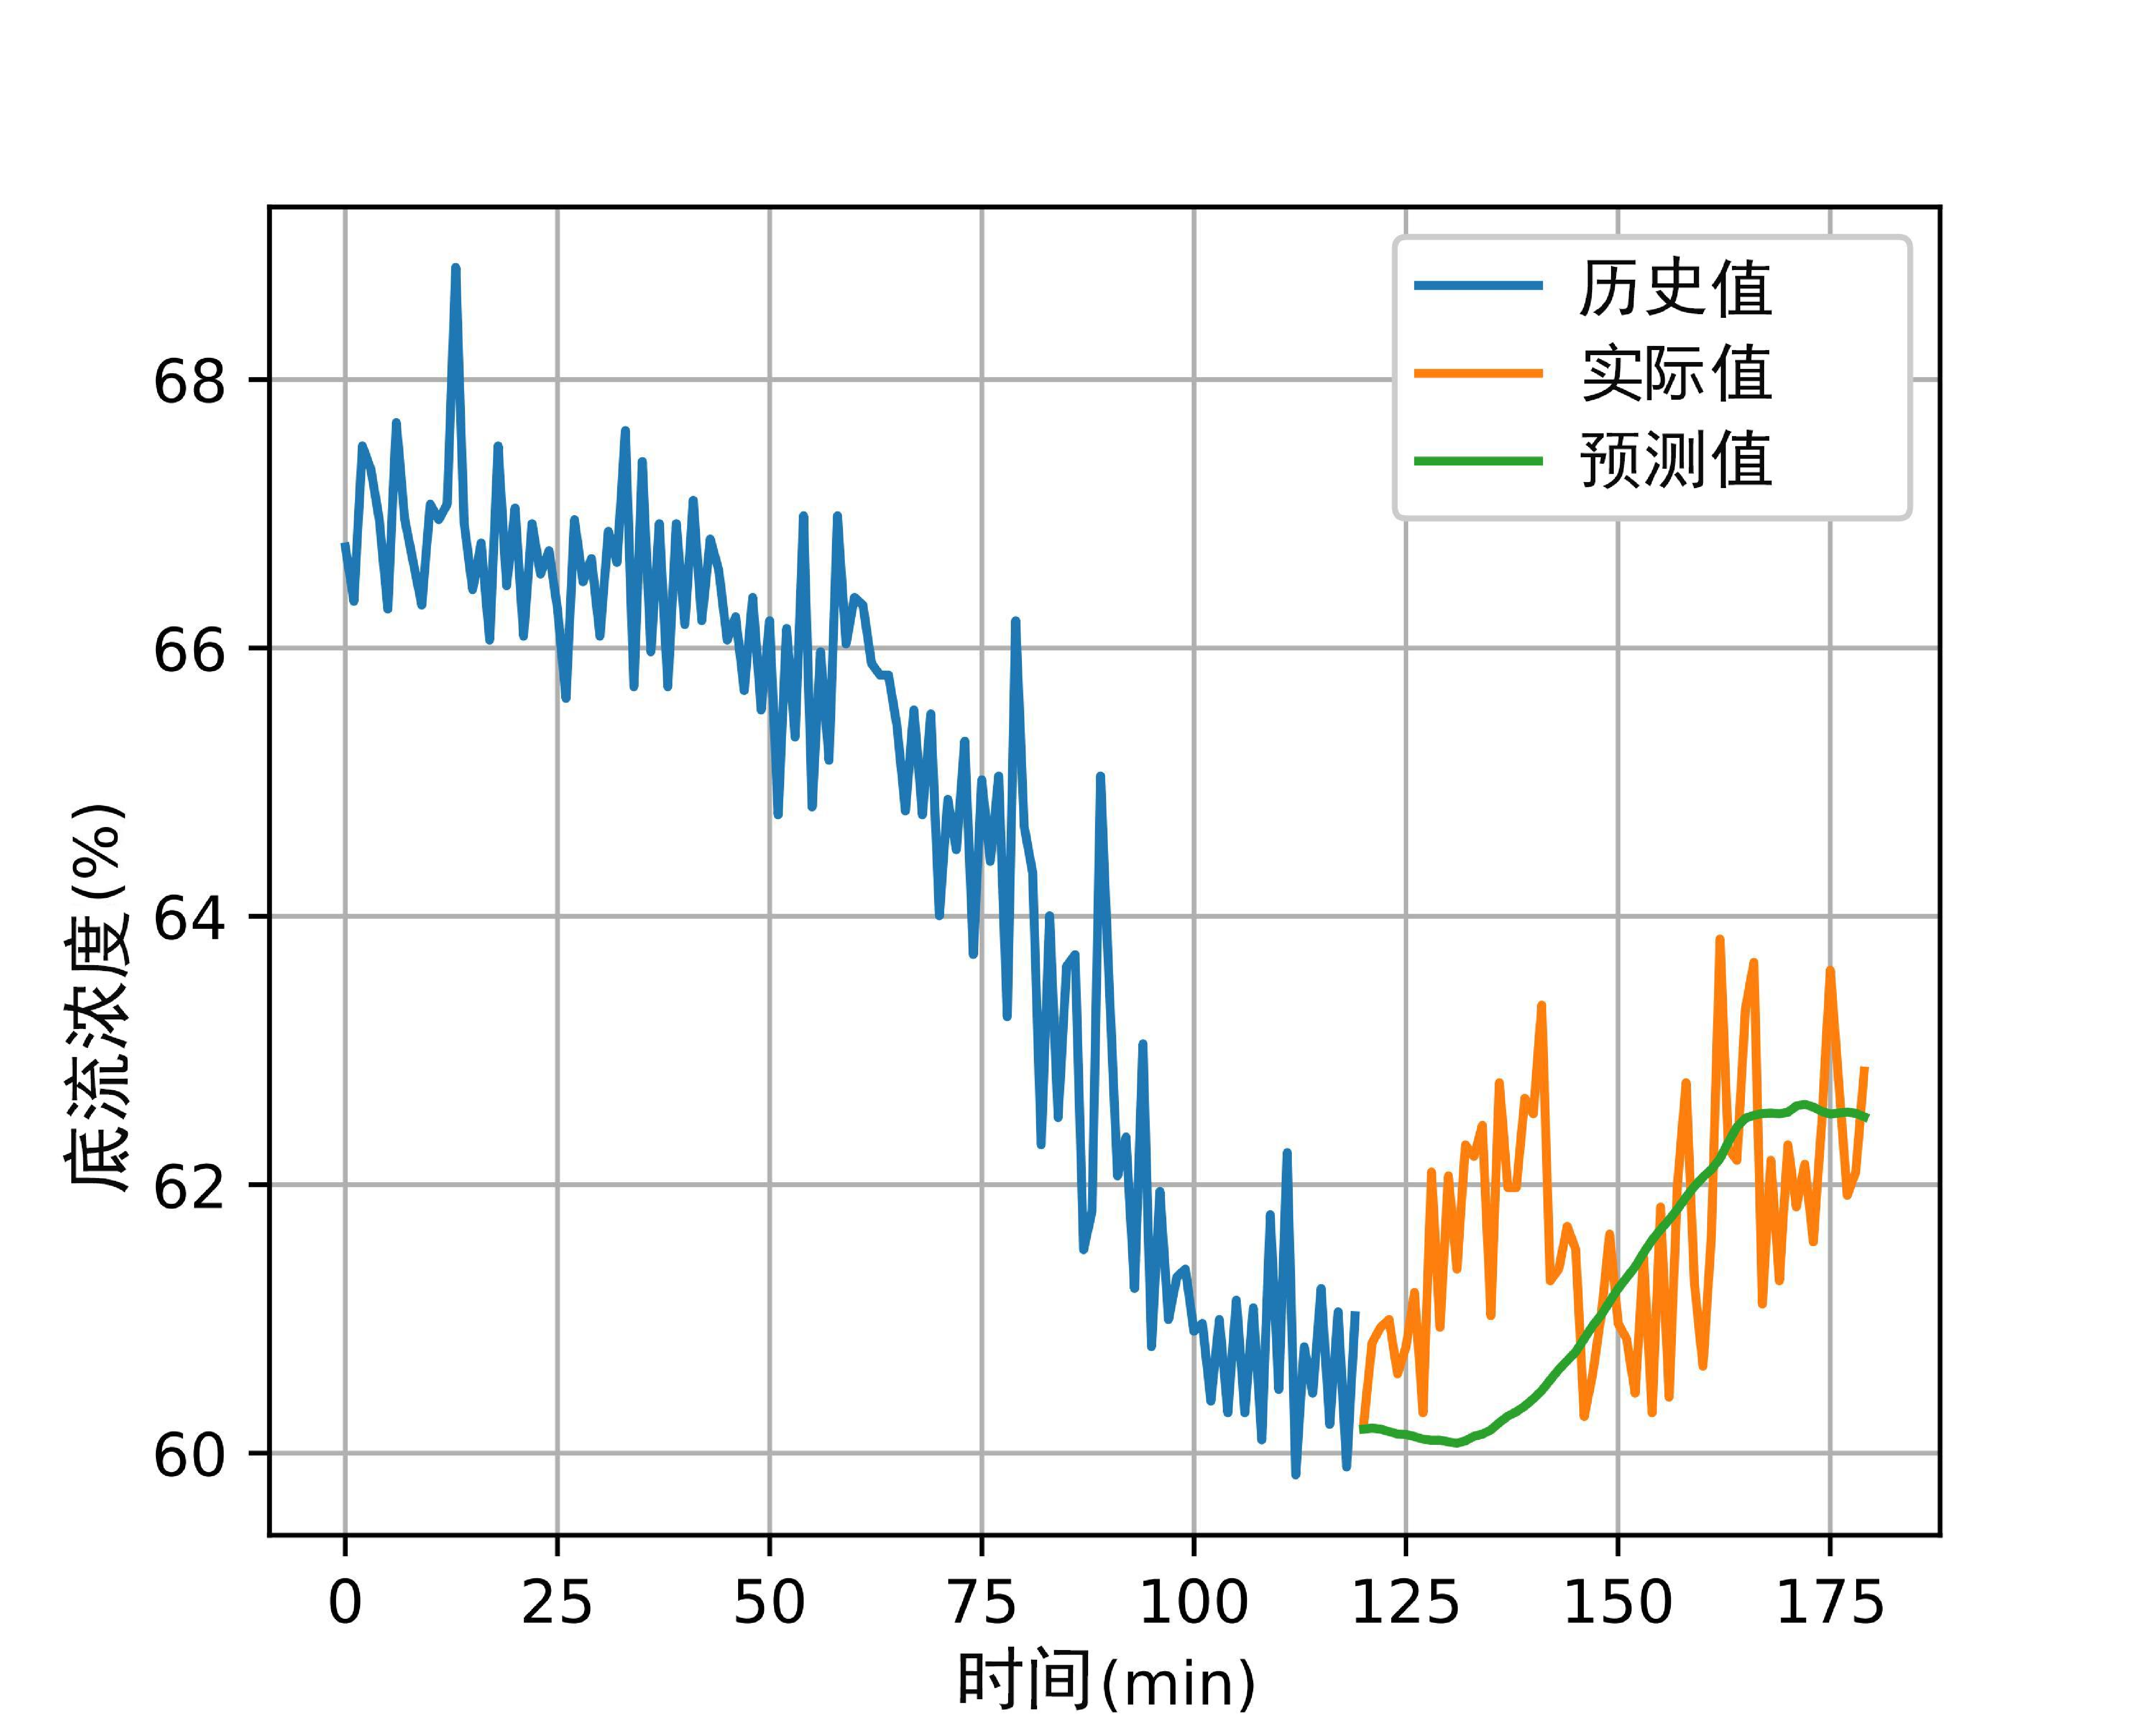
\includegraphics[width=0.49\linewidth,trim=50 0 0 200,clip]{figures/chapter3/predict_cmp/UC_MLP_nonsta_dopri5_60.pdf}
%\caption{fig1}
\end{minipage}
}%
\centering
\caption{不同系统及不同ODE求解器在$L=60$短期预测任务中的性能比较}
\label{fig:predict_cmp_60}
%\vspace*{-0.4cm}
\end{figure}
% k
% \begin{figure}[h]
% \centering
% %\setlength{\abovecaptionskip}{-0.1cm} 
% \subfigure[稳定系统+RK4求解器]{
% \begin{minipage}[t]{0.33\linewidth}
% \centering
% % \hspace{-22pt}
% 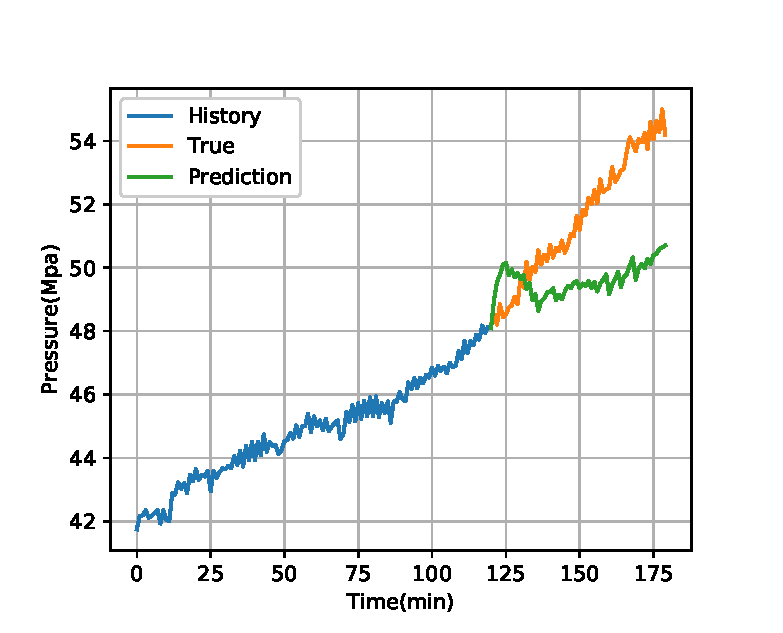
\includegraphics[width=\linewidth,trim=12 0 0 20,clip]{figures/chapter3/predict_cmp/Pressure_GRU_sta_rk4_60.eps}
% % \hspace{-18pt}

% 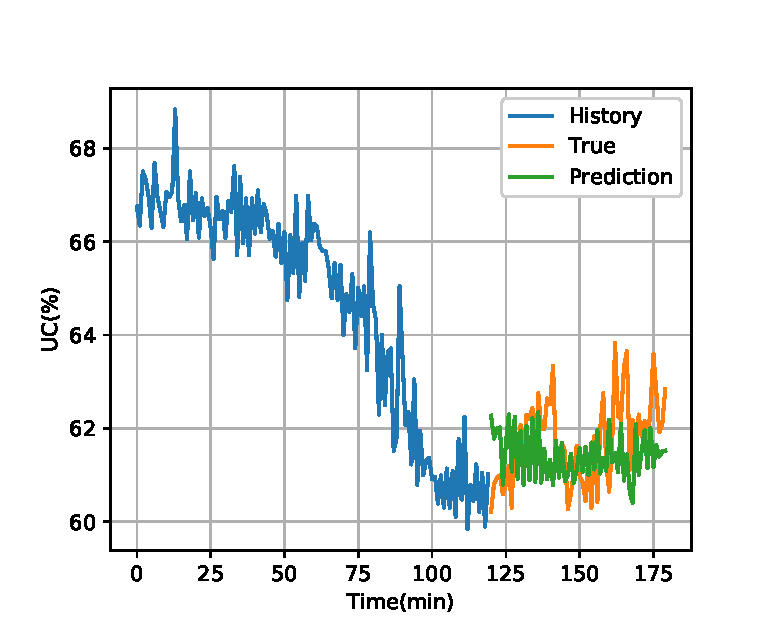
\includegraphics[width=\linewidth,trim=12 0 0 20,clip]{figures/chapter3/predict_cmp/UC_GRU_sta_rk4_60.eps}
% %\caption{fig1}
% \end{minipage}
% }%
% \hspace{-22pt}
% \subfigure[非稳定系统+RK4求解器]{
% \begin{minipage}[t]{0.33\linewidth}
% \centering
% % \hspace{-22pt}
% 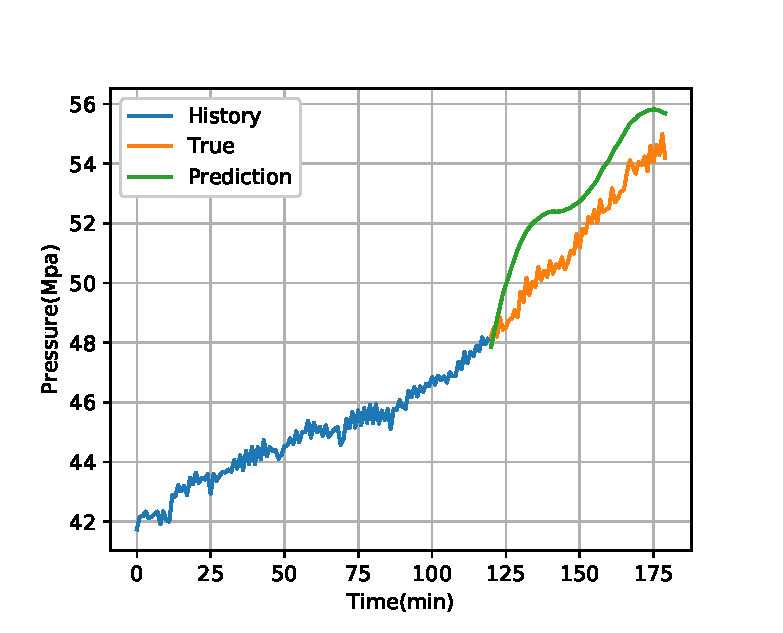
\includegraphics[width=\linewidth,trim=12 0 0 20,clip]{figures/chapter3/predict_cmp/Pressure_MLP_nonsta_rk4_60.eps}
% % \hspace{-18pt}

% 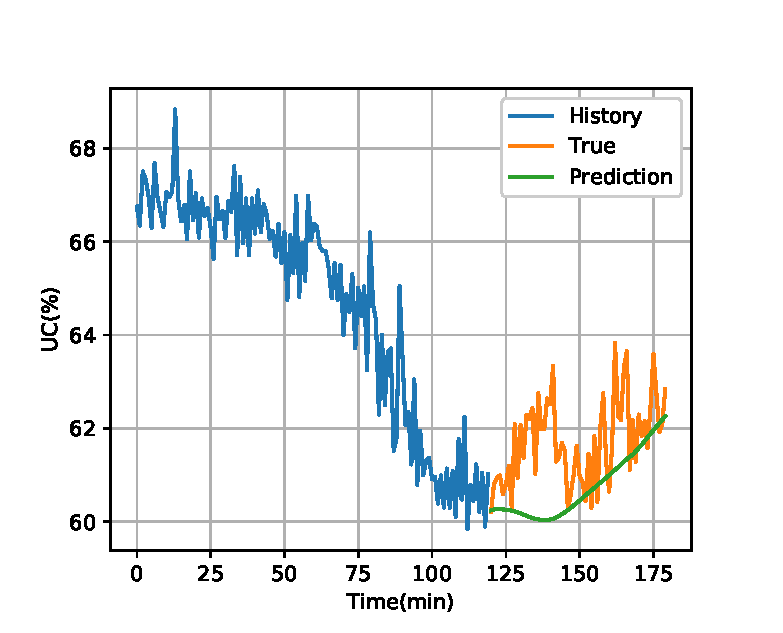
\includegraphics[width=\linewidth,trim=12 0 0 20,clip]{figures/chapter3/predict_cmp/UC_MLP_nonsta_rk4_60.eps}
% %\caption{fig1}
% \end{minipage}
% }%
% \hspace{-22pt}
% \subfigure[非稳定系统+Dopri5求解器]{
% \begin{minipage}[t]{0.33\linewidth}
% \centering
% % \hspace{-22pt}
% 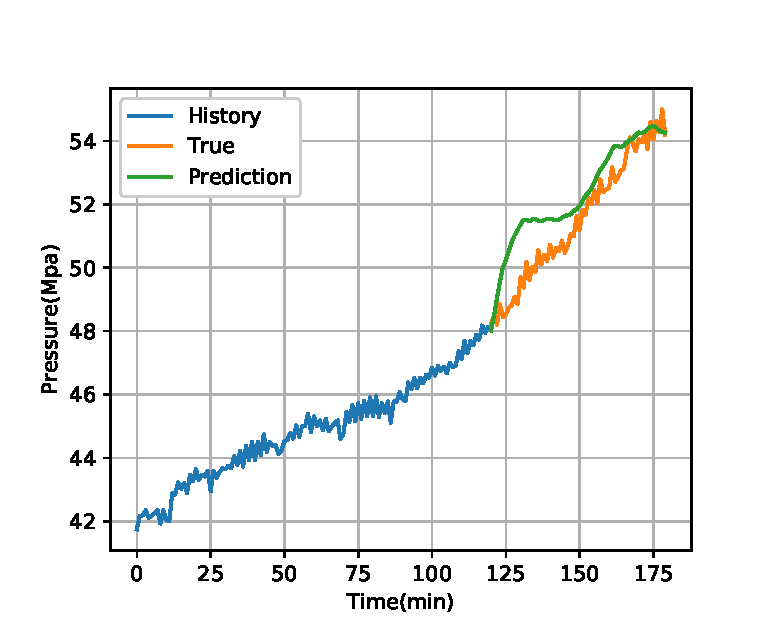
\includegraphics[width=\linewidth,trim=12 0 0 20,clip]{figures/chapter3/predict_cmp/Pressure_MLP_nonsta_dopri5_60.eps}
% % \hspace{-18pt}

% 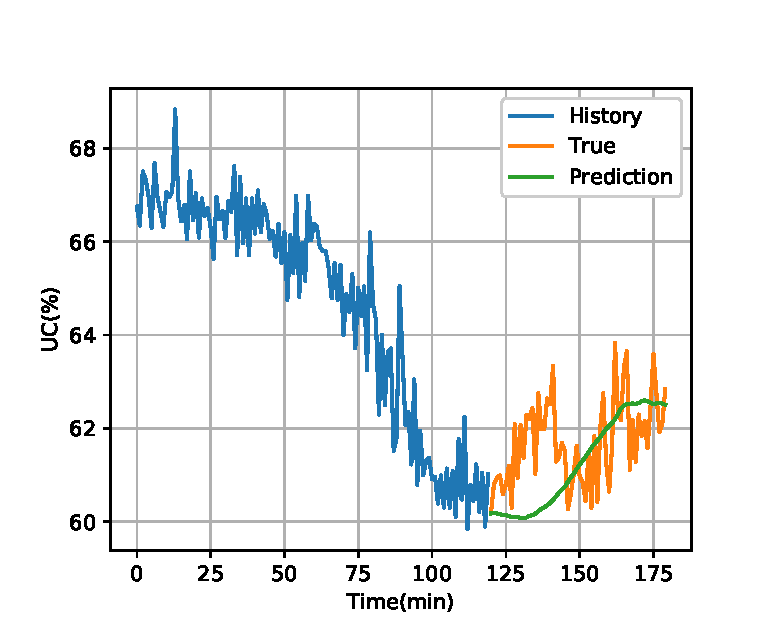
\includegraphics[width=\linewidth,trim=12 0 0 20,clip]{figures/chapter3/predict_cmp/UC_MLP_nonsta_dopri5_60.eps}
% %\caption{fig1}
% \end{minipage}
% }%
% \centering
% \caption{不同系统及不同ODE求解器在$L=60$短期预测任务中的性能比较}
% \label{fig:predict_cmp_60}
% %\vspace*{-0.4cm}
% \end{figure}

结果表明,非平稳模型在短期预测任务中的表现优于平稳模型,预测得到的序列相比平稳模型更接近实际系统输出。
% The non-stationary system learns the evolution of internal hidden state which 
% The model with non-stationary system dynamic identifies the system smoothly because the structures constraint hidden state can only change in a continuous and slow form.
% TODO: 真的不想删,但是受篇幅限制暂时注释,以后有机会偷偷补上
此外,由于非稳定系统结构限制了隐状态只能以连续、缓慢的方式变化。该约束符合浓密机系统运行缓慢的特性,等价于减小模型参数的搜索空间,抑制模型过拟合的情况。
图\ref{fig:predict_cmp_200}展示了在长期预测任务($L=200$)中的模型预测结果。
% ($L=500$的类似结果可以在Table~\ref{tab:3_exp_all}中找到)。
\begin{figure}[htpb]
%\setlength{\abovecaptionskip}{-0.1cm} 
\centering
\subfigure[非稳定系统+RK4求解器]{
\begin{minipage}[t]{\linewidth}
\centering
% \hspace{-22pt}
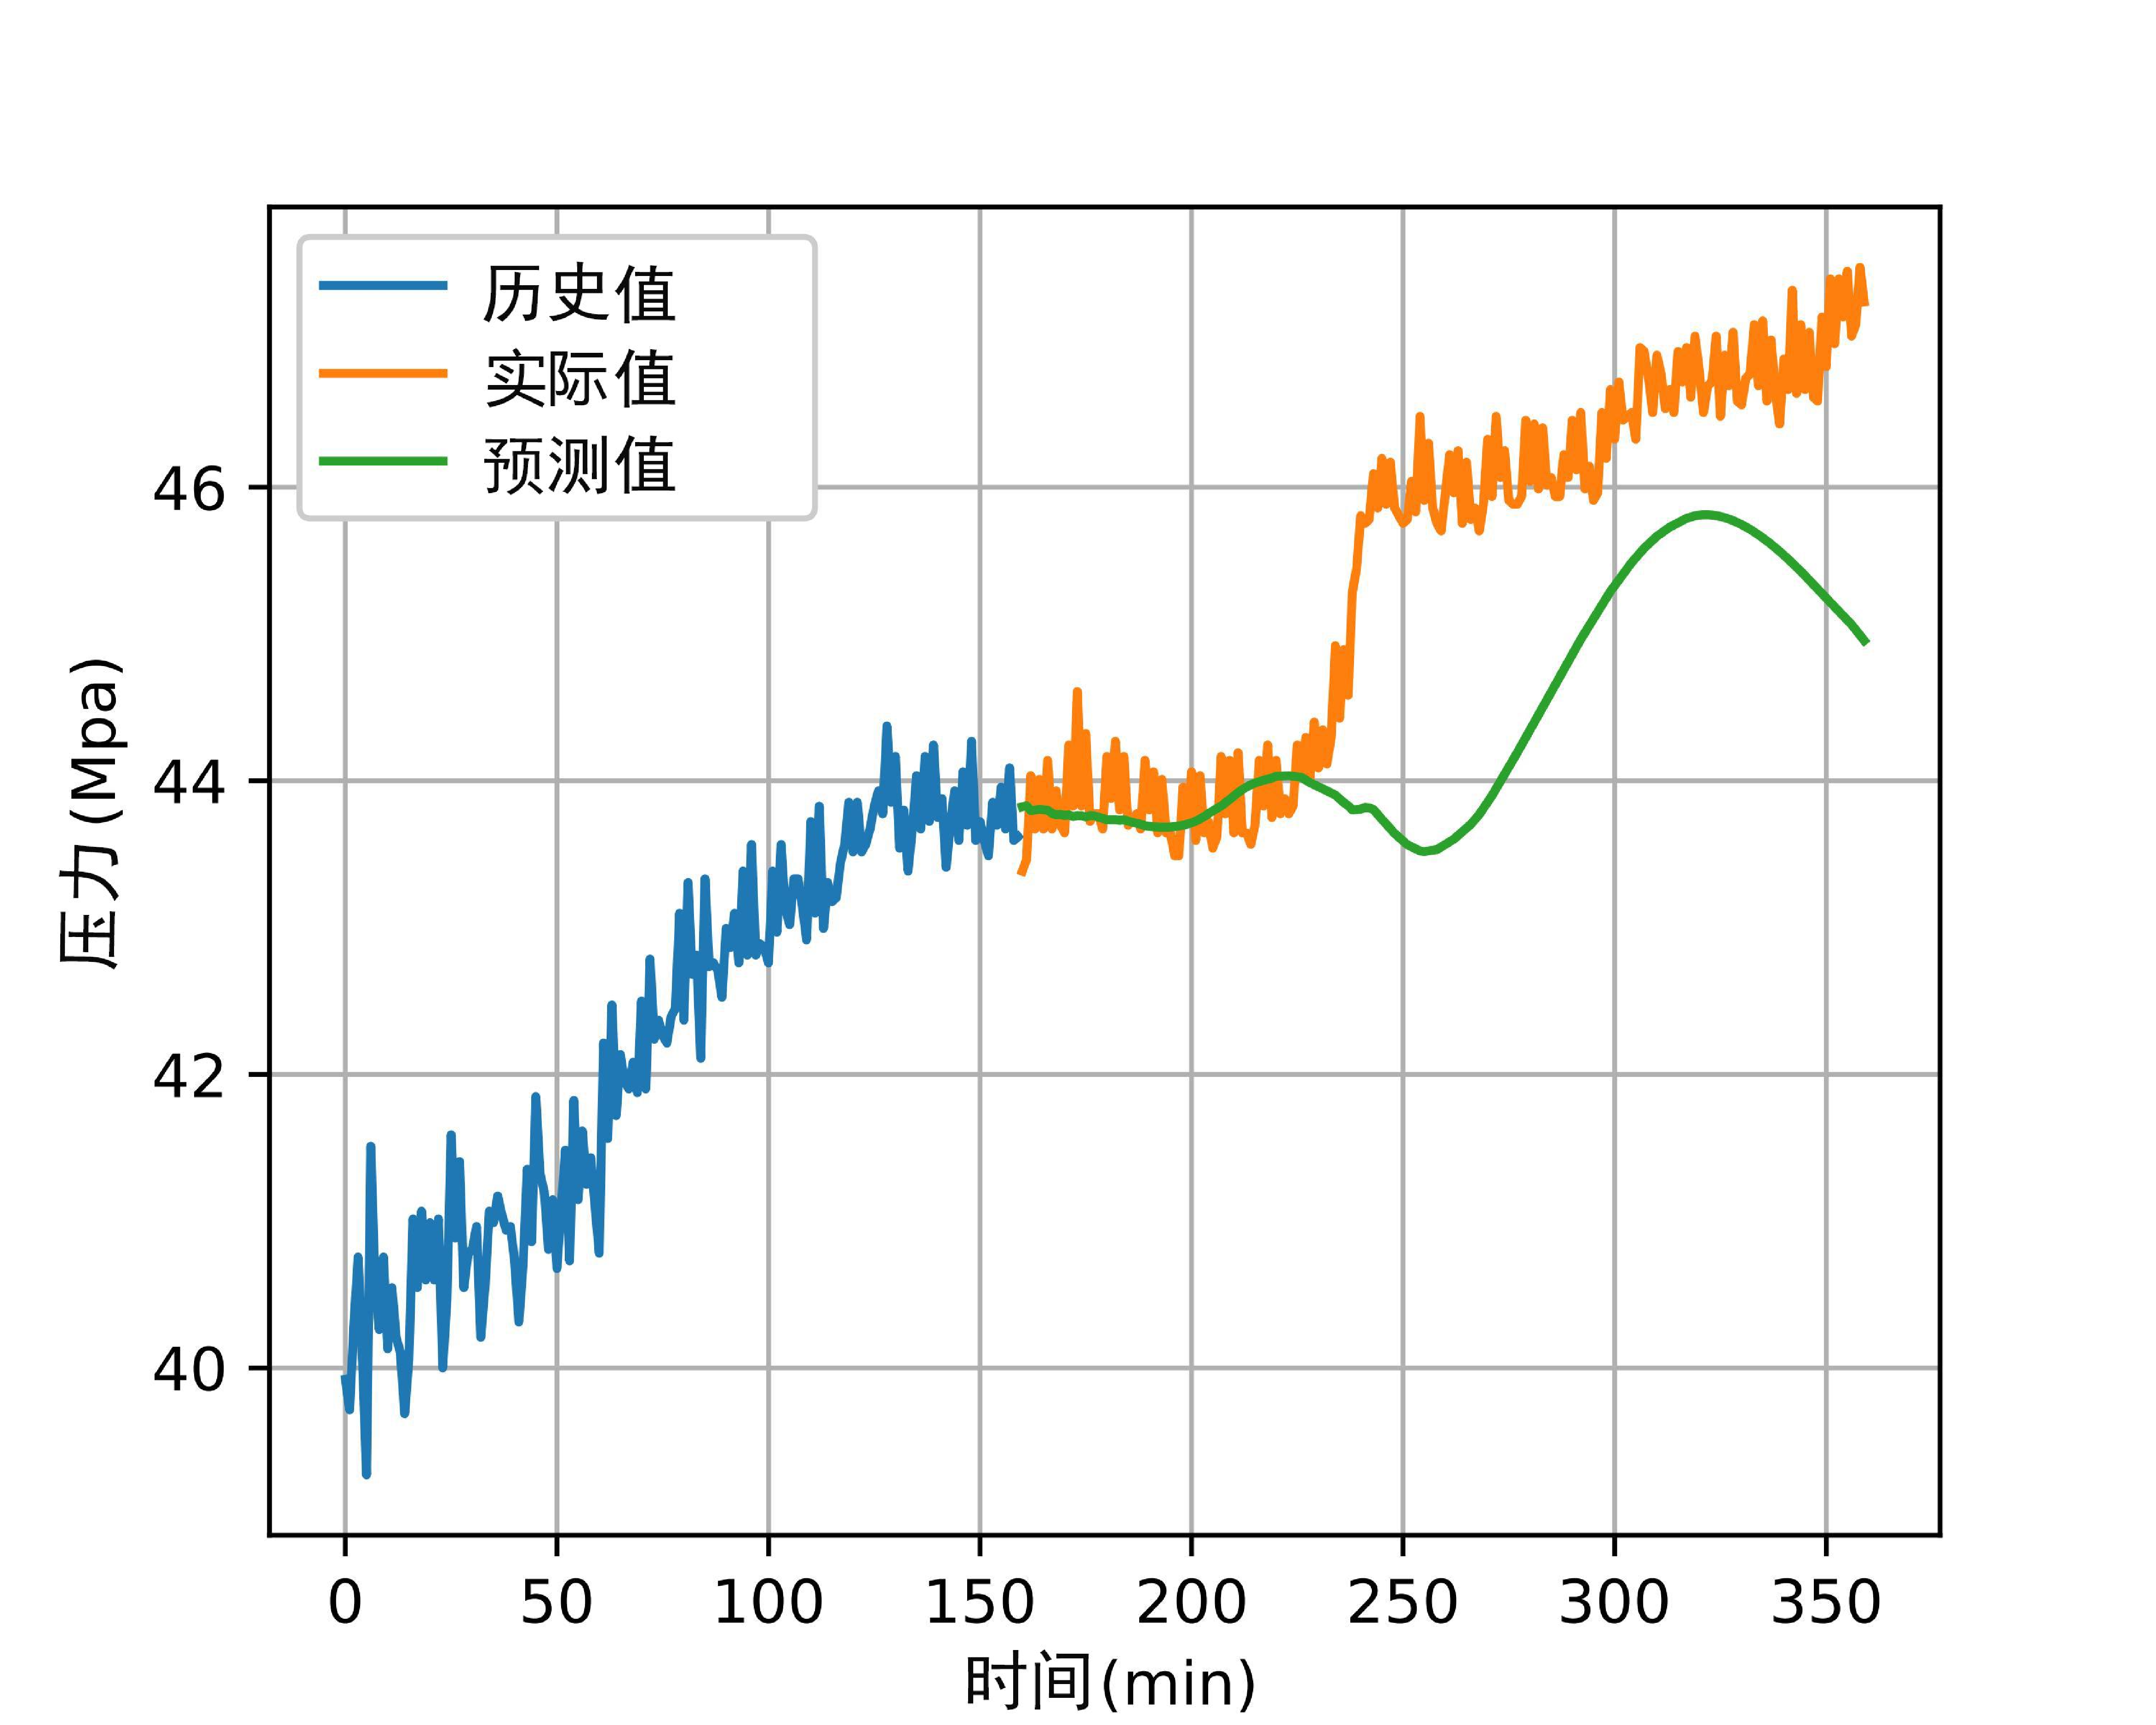
\includegraphics[width=0.49\linewidth,trim=50 0 0 200,clip]{figures/chapter3/predict_cmp/Pressure_MLP_nonsta_rk4_200.pdf}
% \hspace{-18pt}
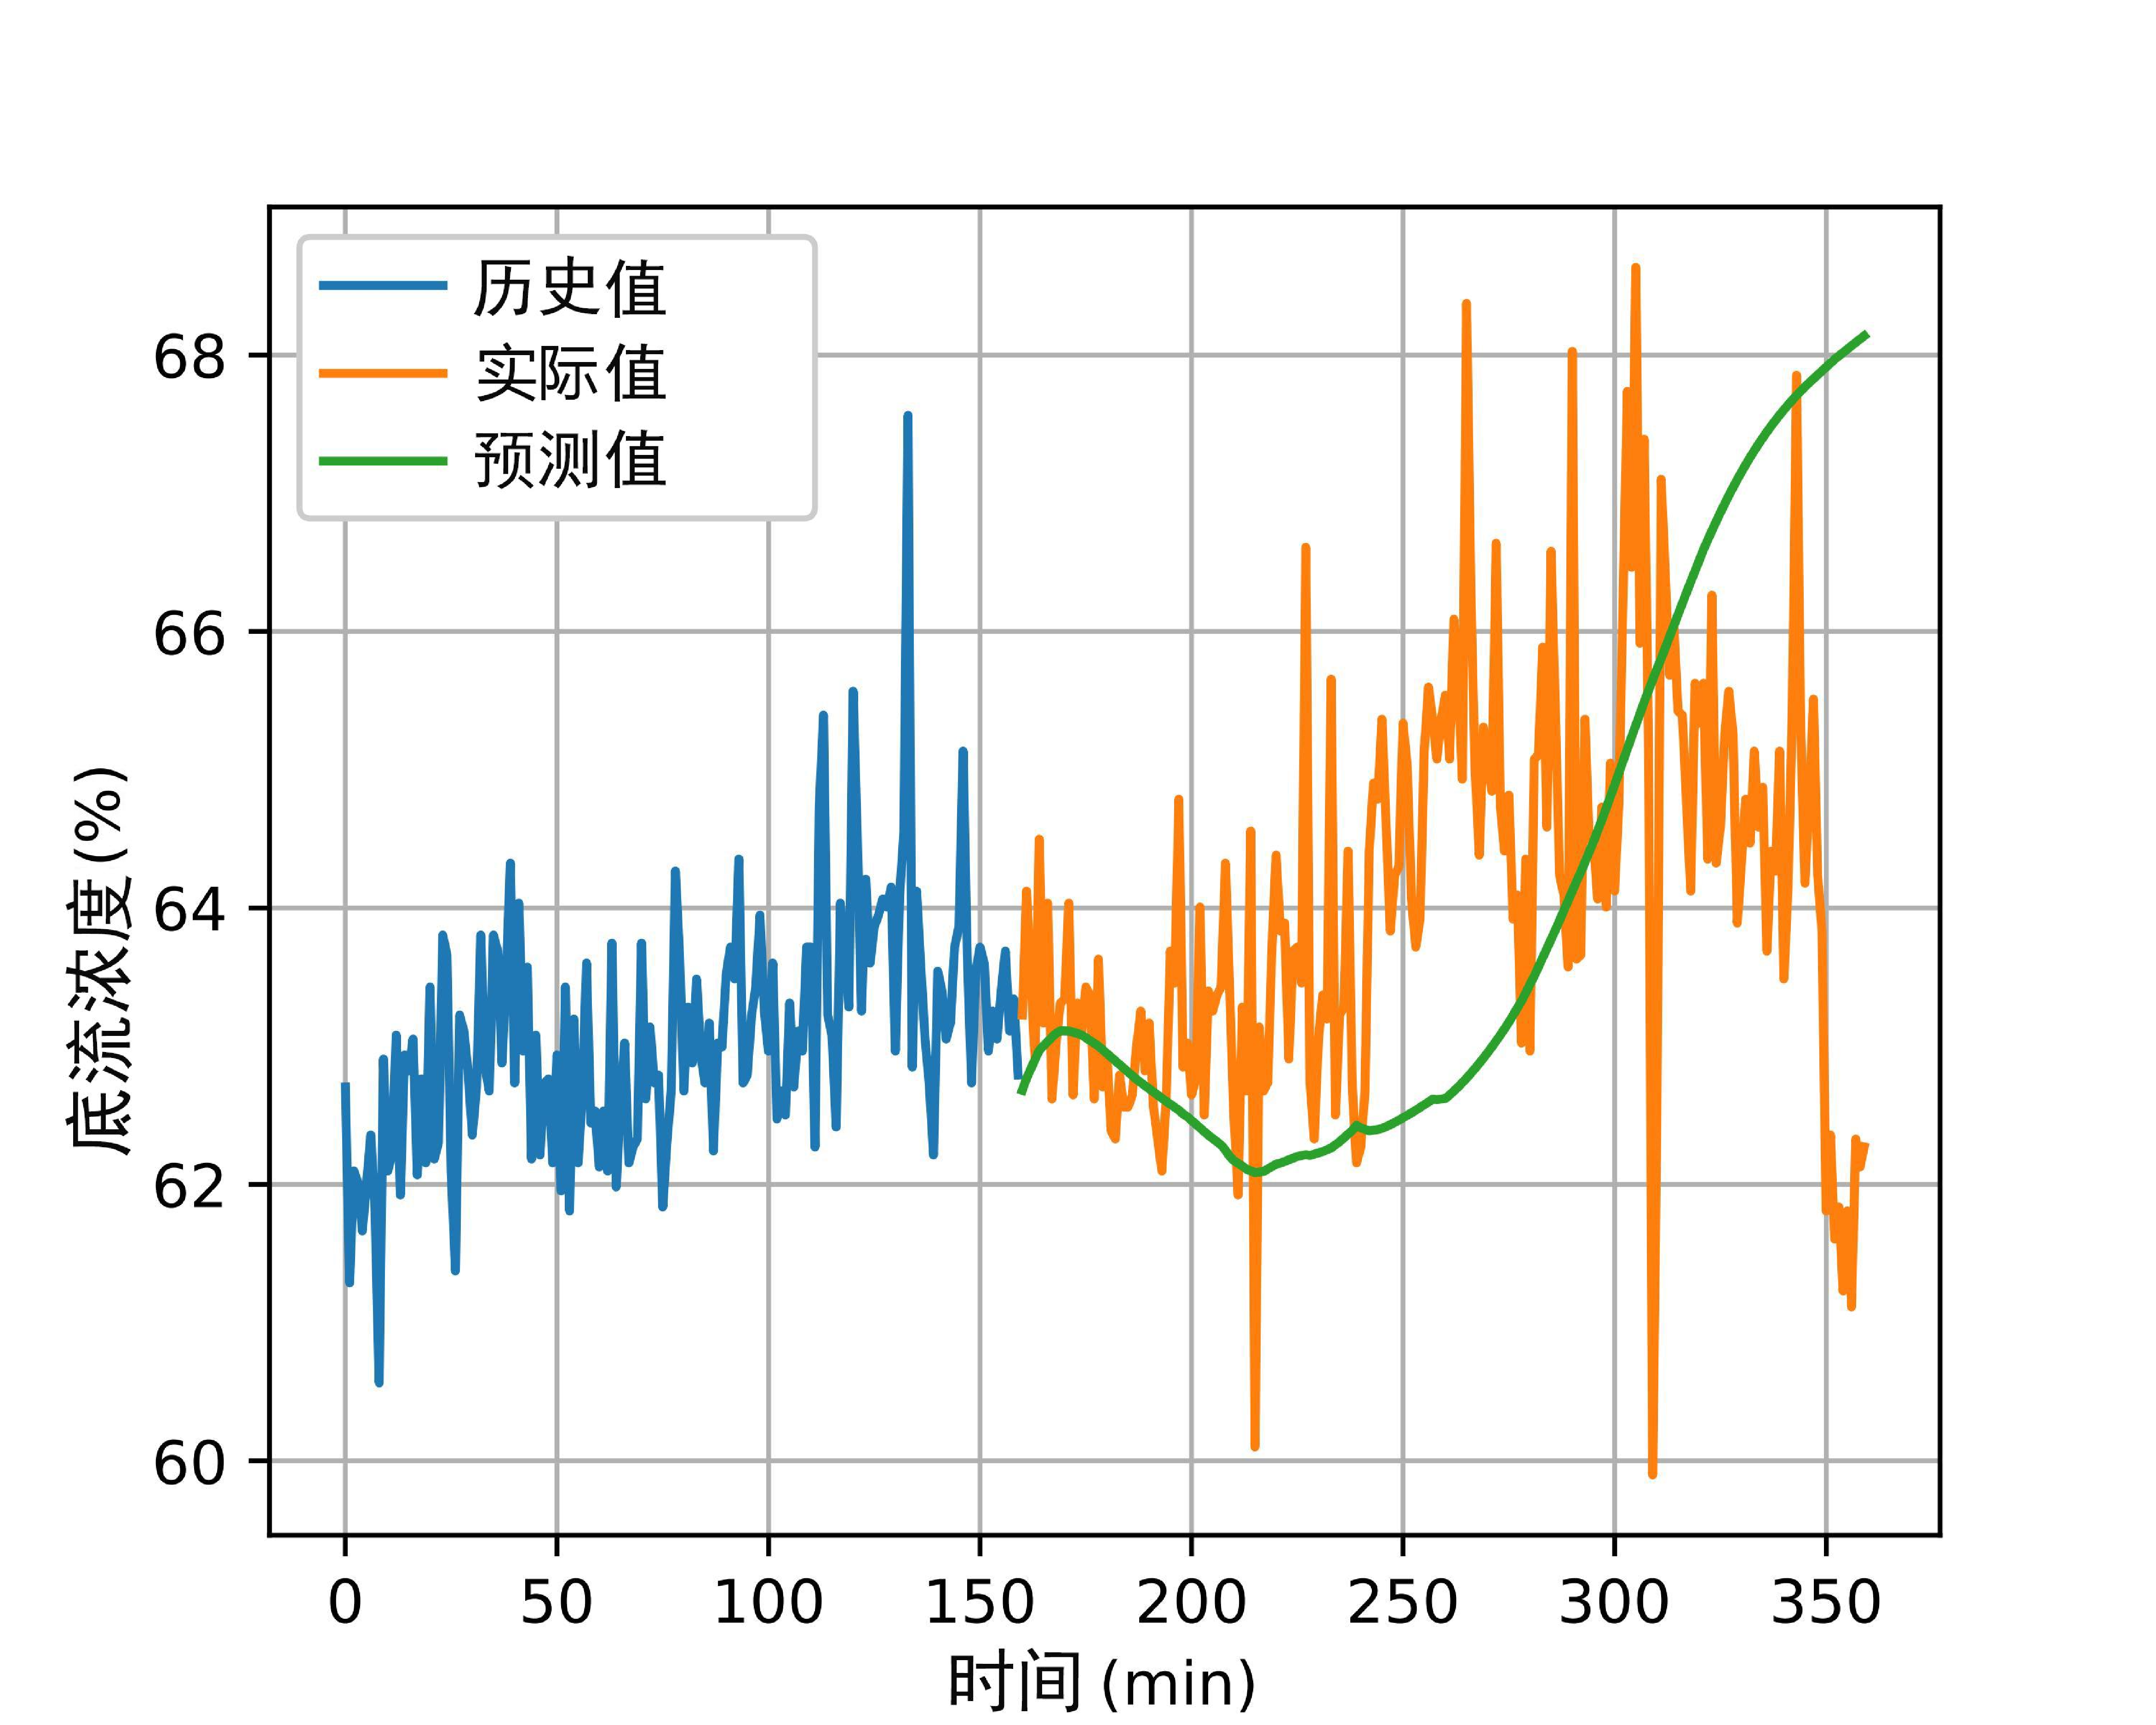
\includegraphics[width=0.45\linewidth,trim=50 0 0 200,clip]{figures/chapter3/predict_cmp/UC_MLP_nonsta_rk4_200.pdf}
%\caption{fig:subfig_200_nonsta_rk4}
\end{minipage}
\label{fig:subfig_200_nonsta_rk4}
}%
% \hspace{-22pt}

\subfigure[稳定系统+Euler求解器]{
\begin{minipage}[t]{\linewidth}
\centering
% \hspace{-22pt}
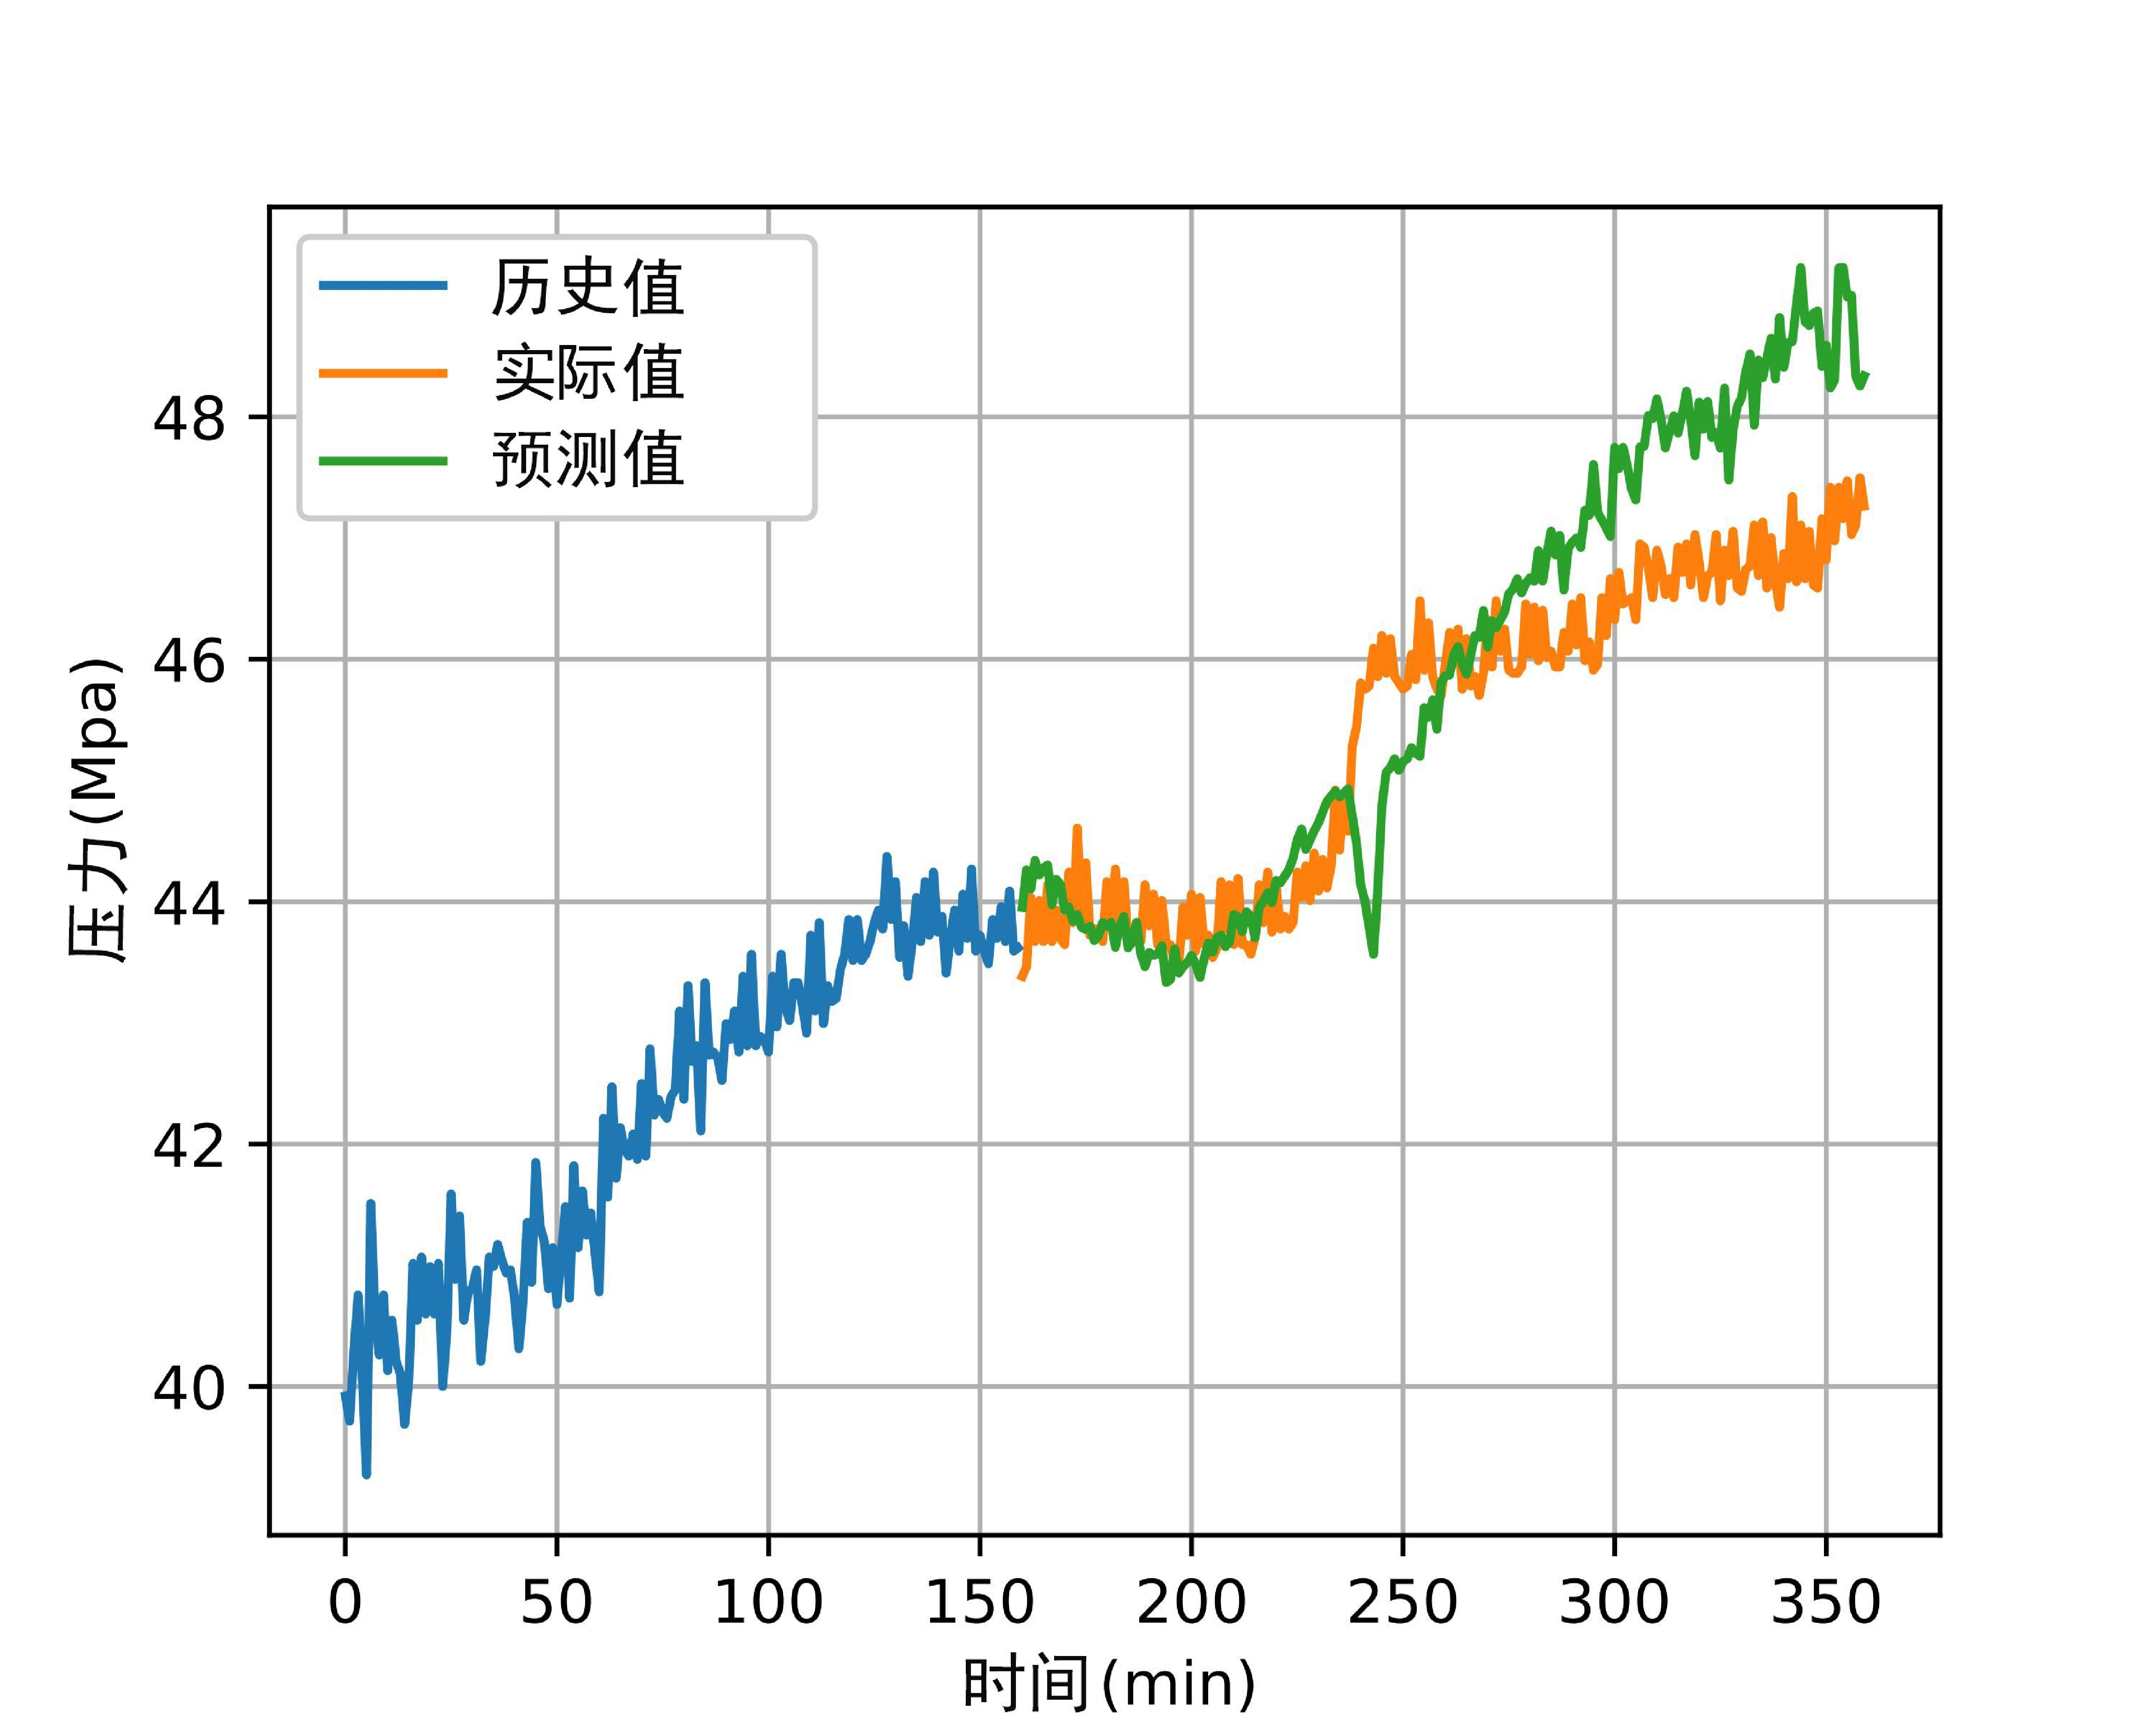
\includegraphics[width=0.45\linewidth,trim=50 0 0 200,clip]{figures/chapter3/predict_cmp/Pressure_GRU_sta_euler_200.pdf}
% \hspace{-18pt}
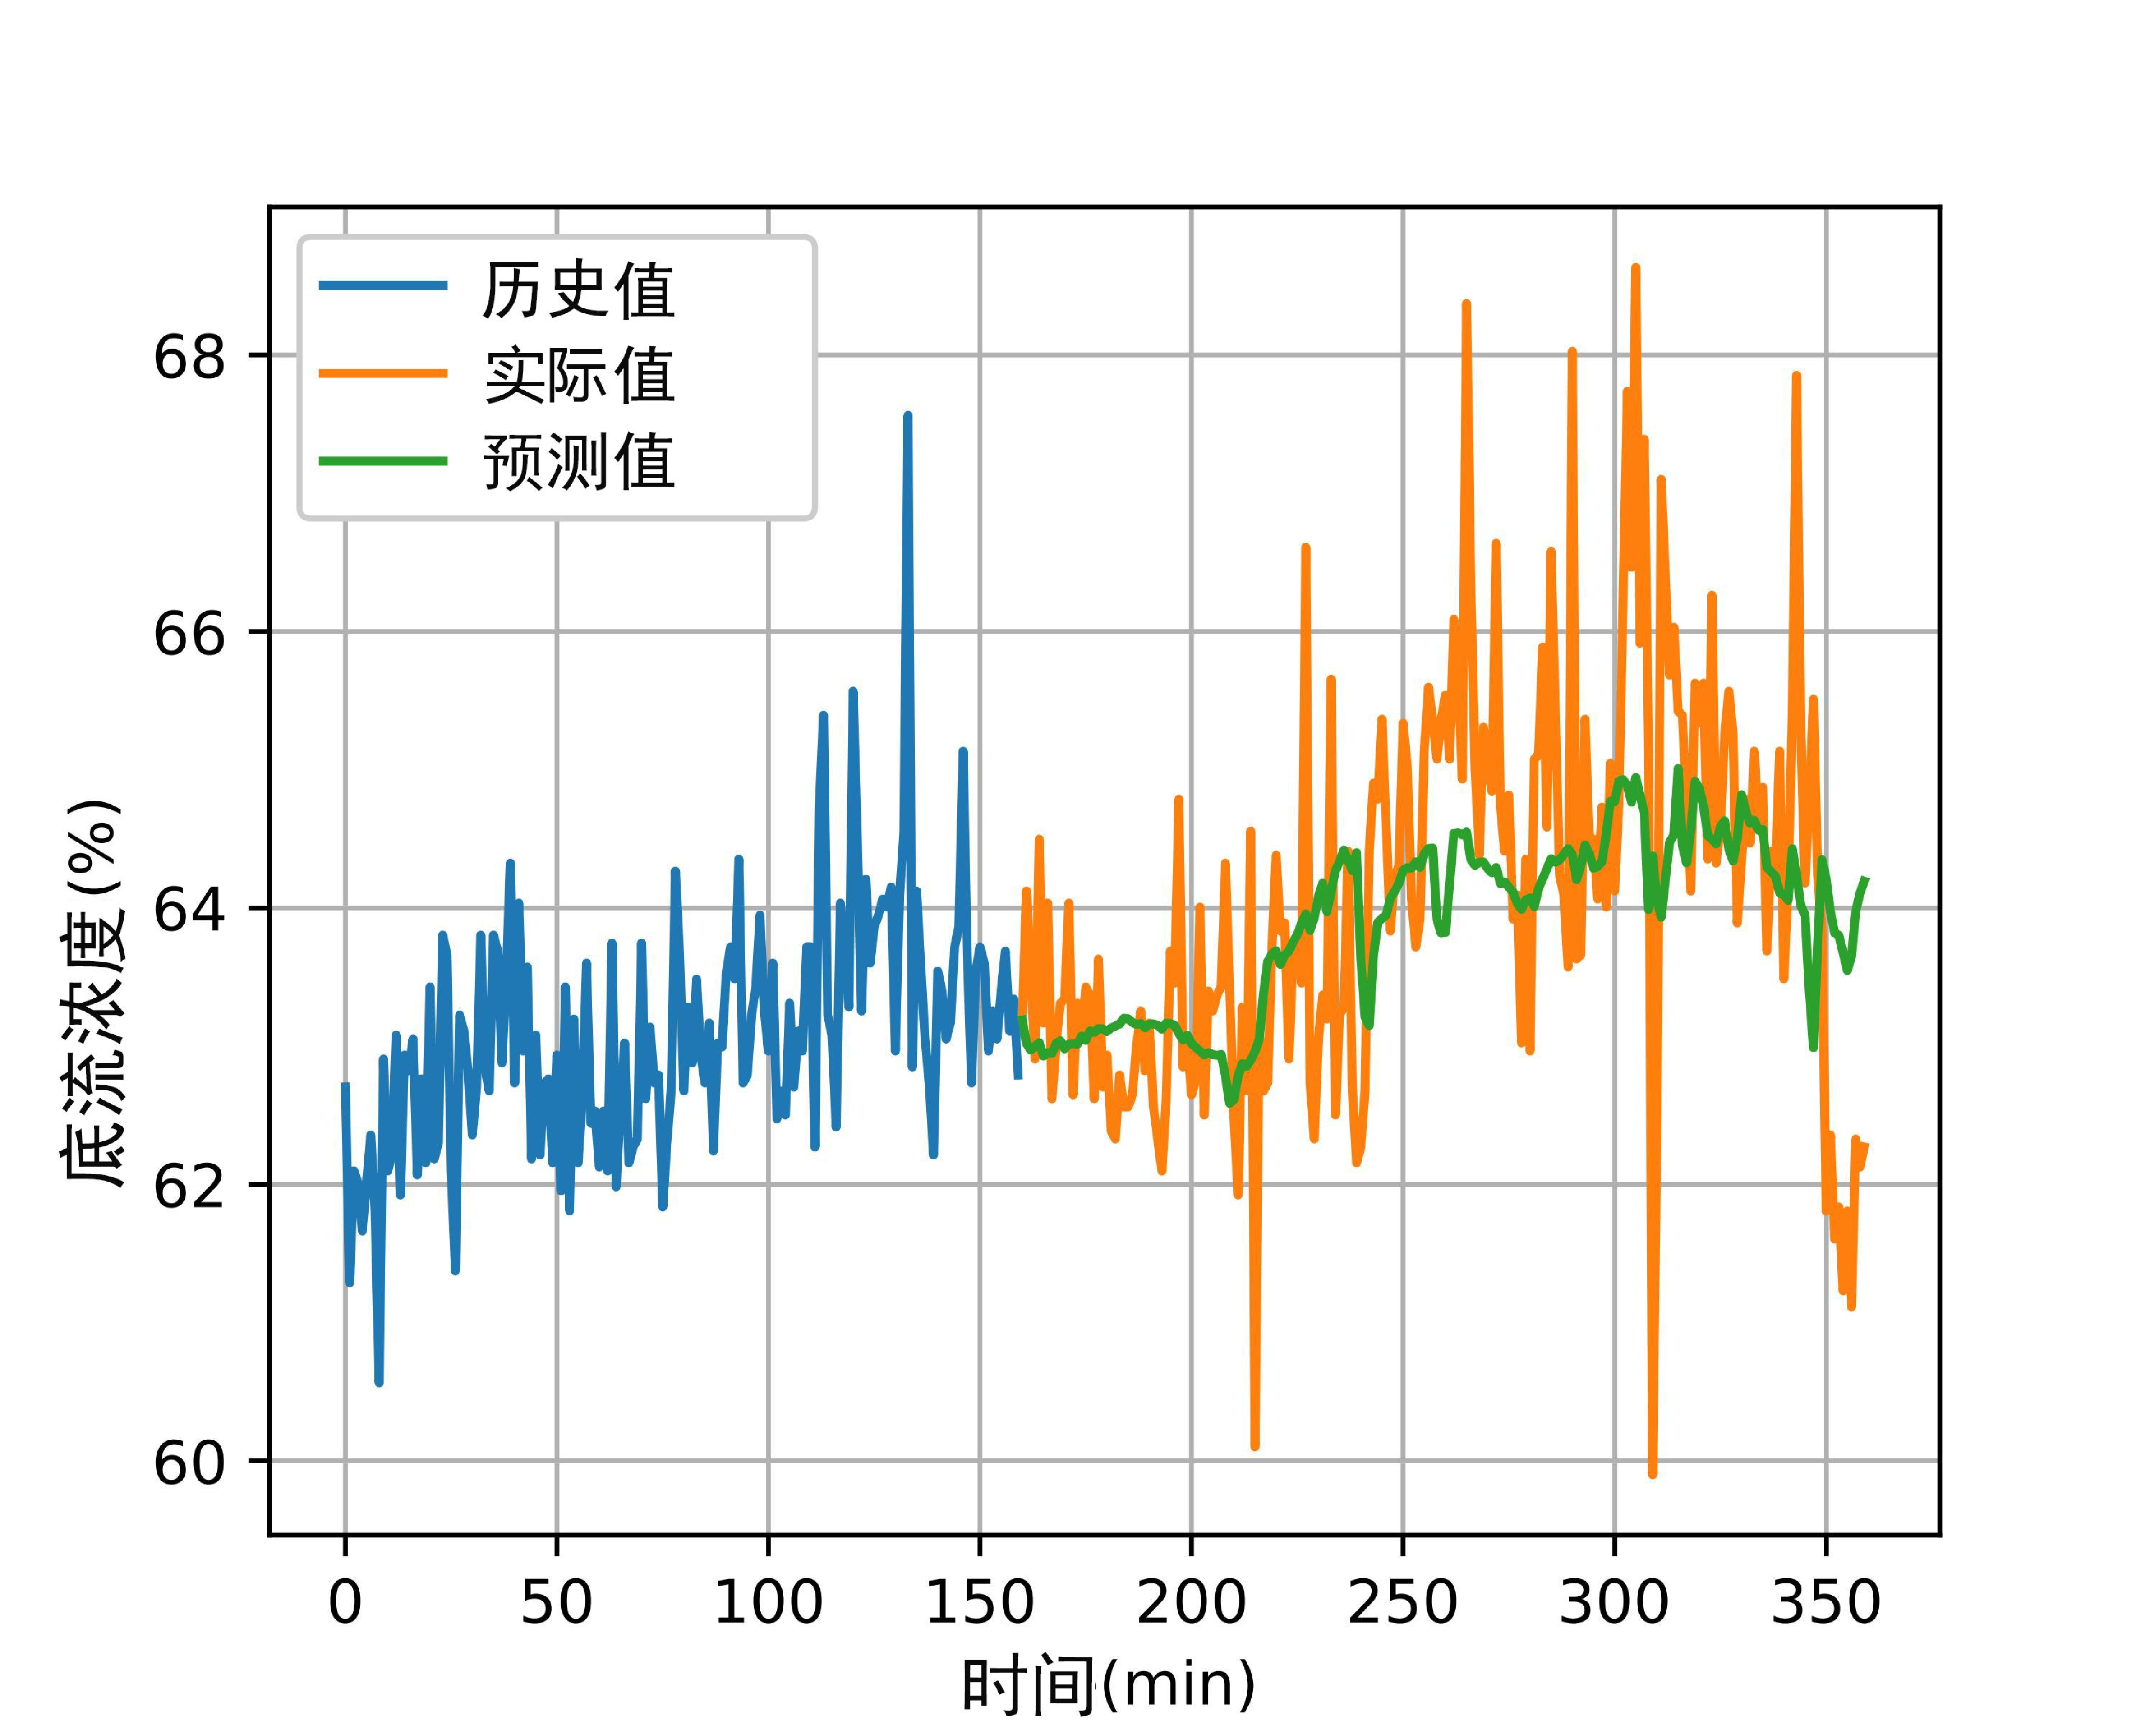
\includegraphics[width=0.45\linewidth,trim=50 0 0 200,clip]{figures/chapter3/predict_cmp/UC_GRU_sta_euler_200.pdf}
%\caption{fig:subfig_200_sta_euler}
\end{minipage}%
\label{fig:subfig_200_sta_euler}
}%

\hspace{-22pt}
\subfigure[稳定系统+RK4求解器]{
\begin{minipage}[t]{\linewidth}
\centering
% \hspace{-22pt}
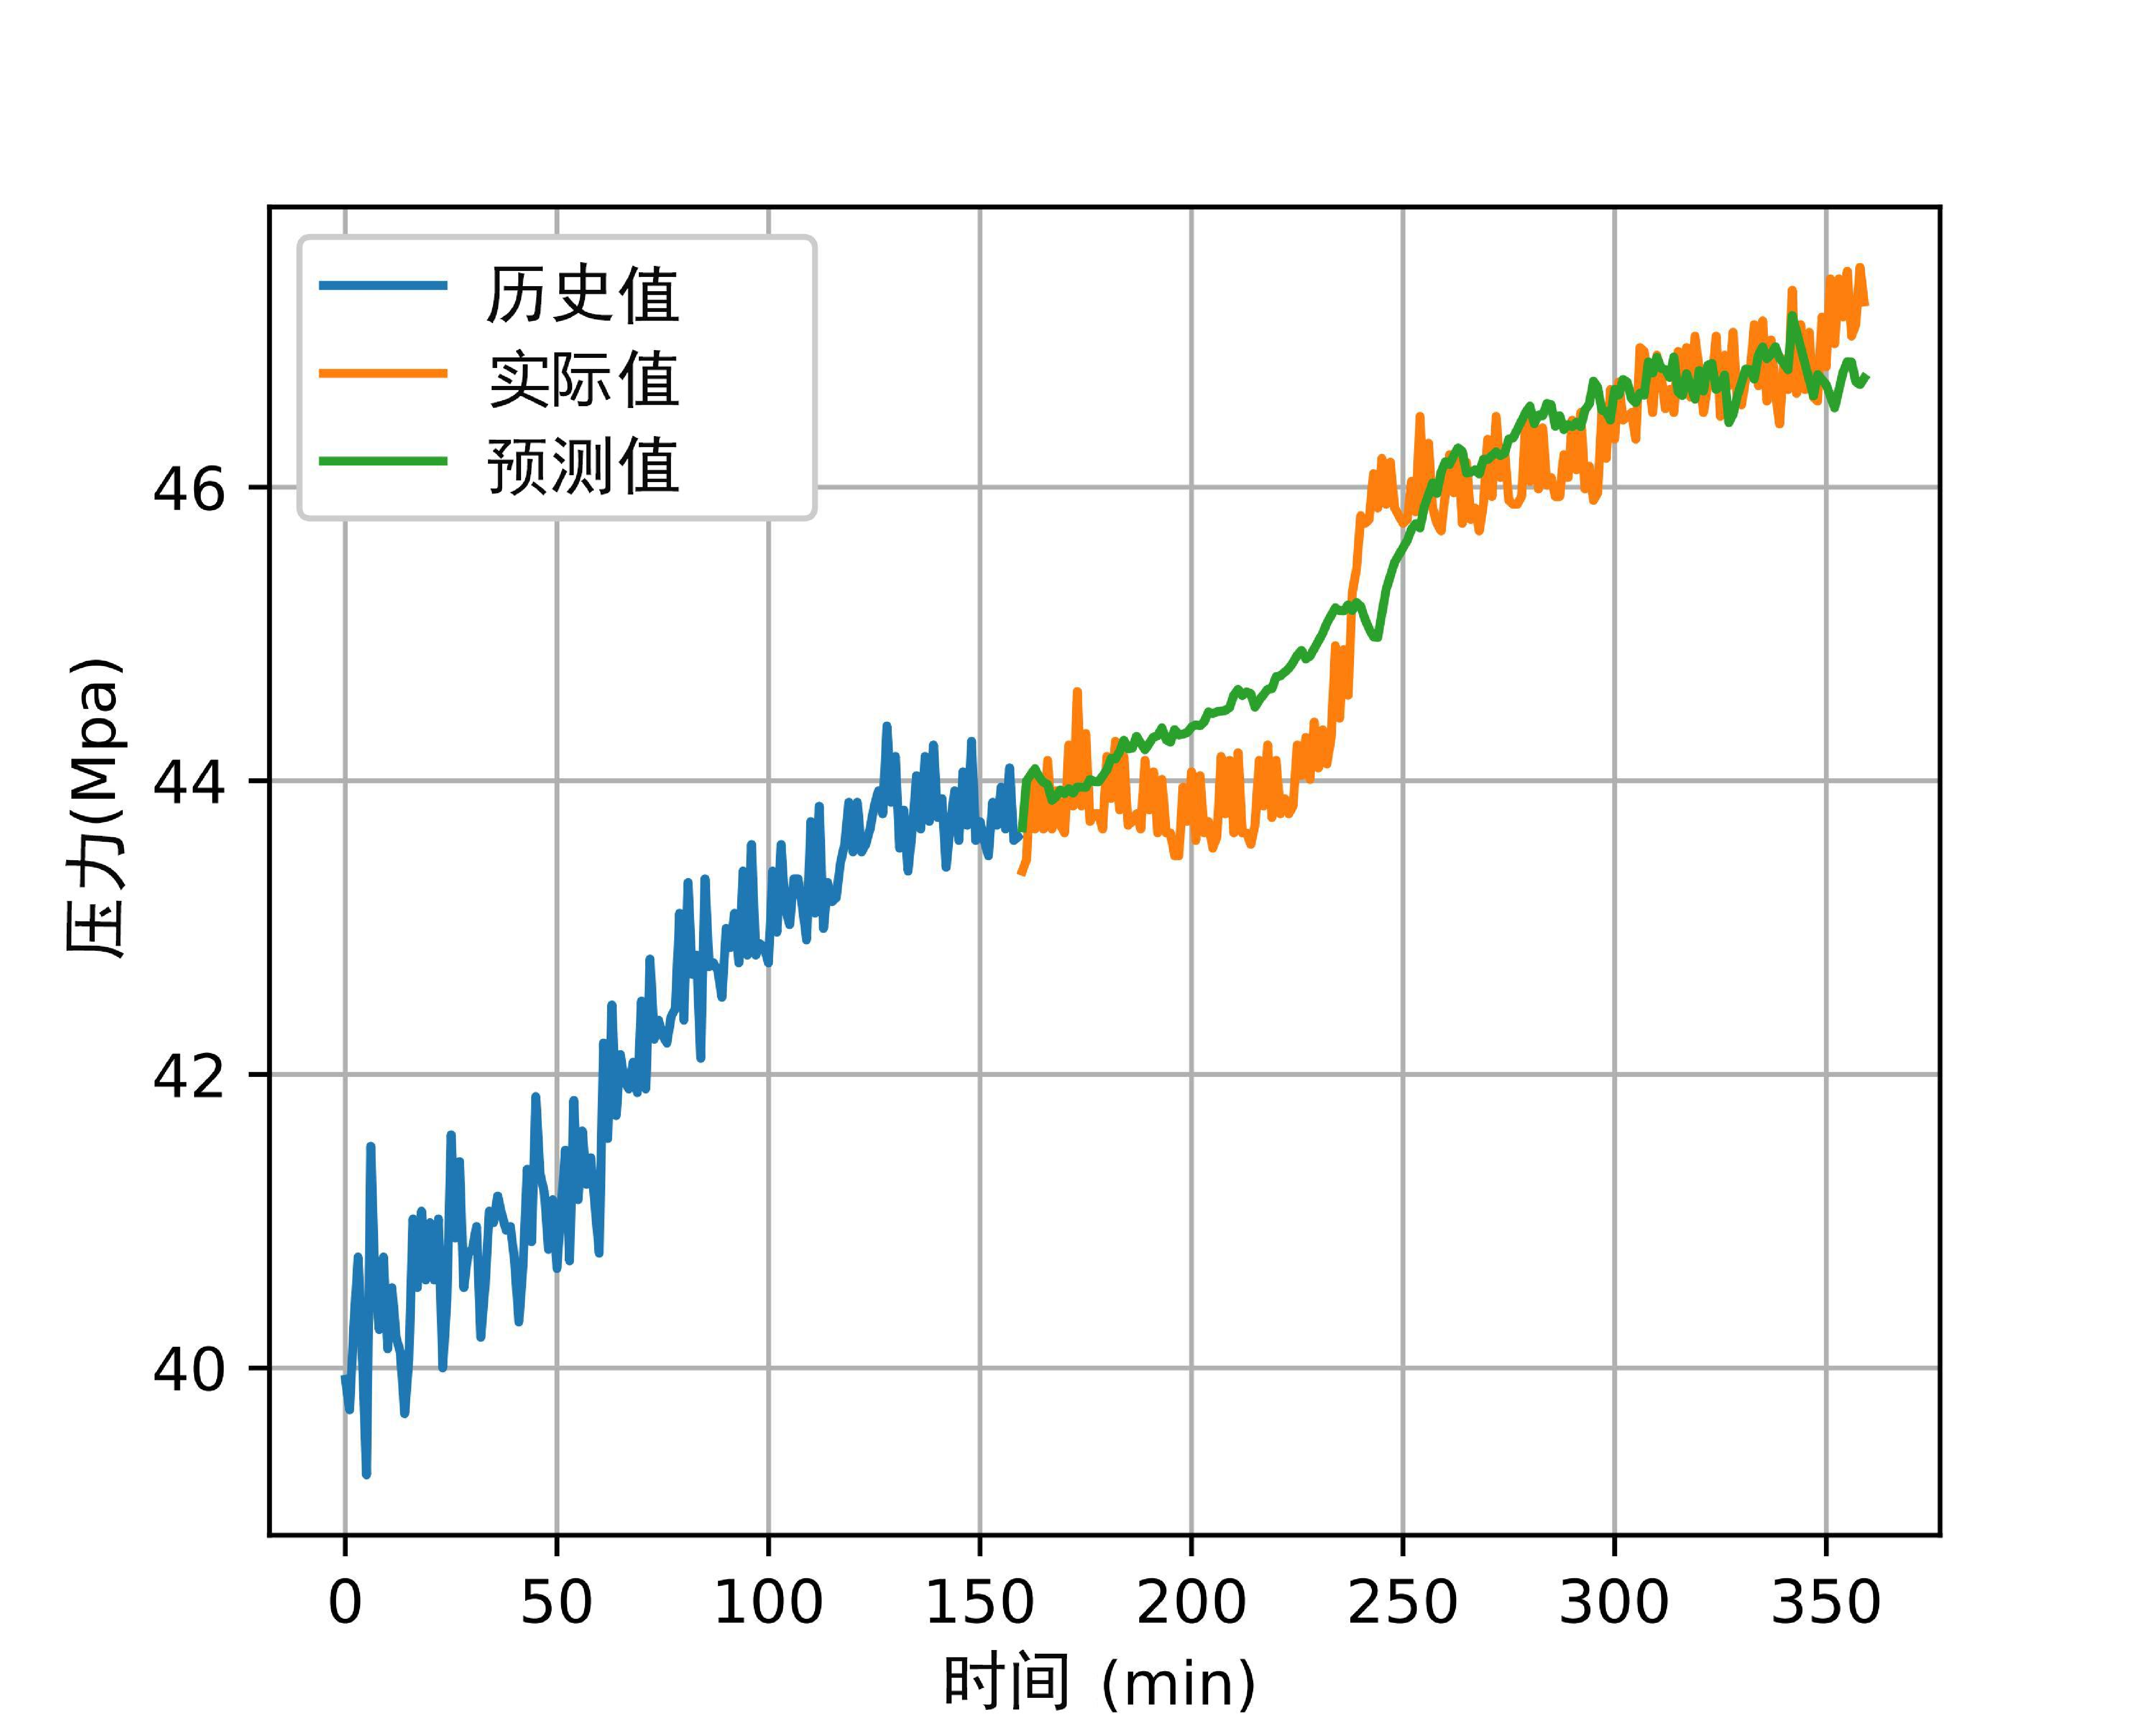
\includegraphics[width=0.45\linewidth,trim=50 0 0 200,clip]{figures/chapter3/predict_cmp/Pressure_GRU_sta_rk4_200.pdf}
% \hspace{-18pt}
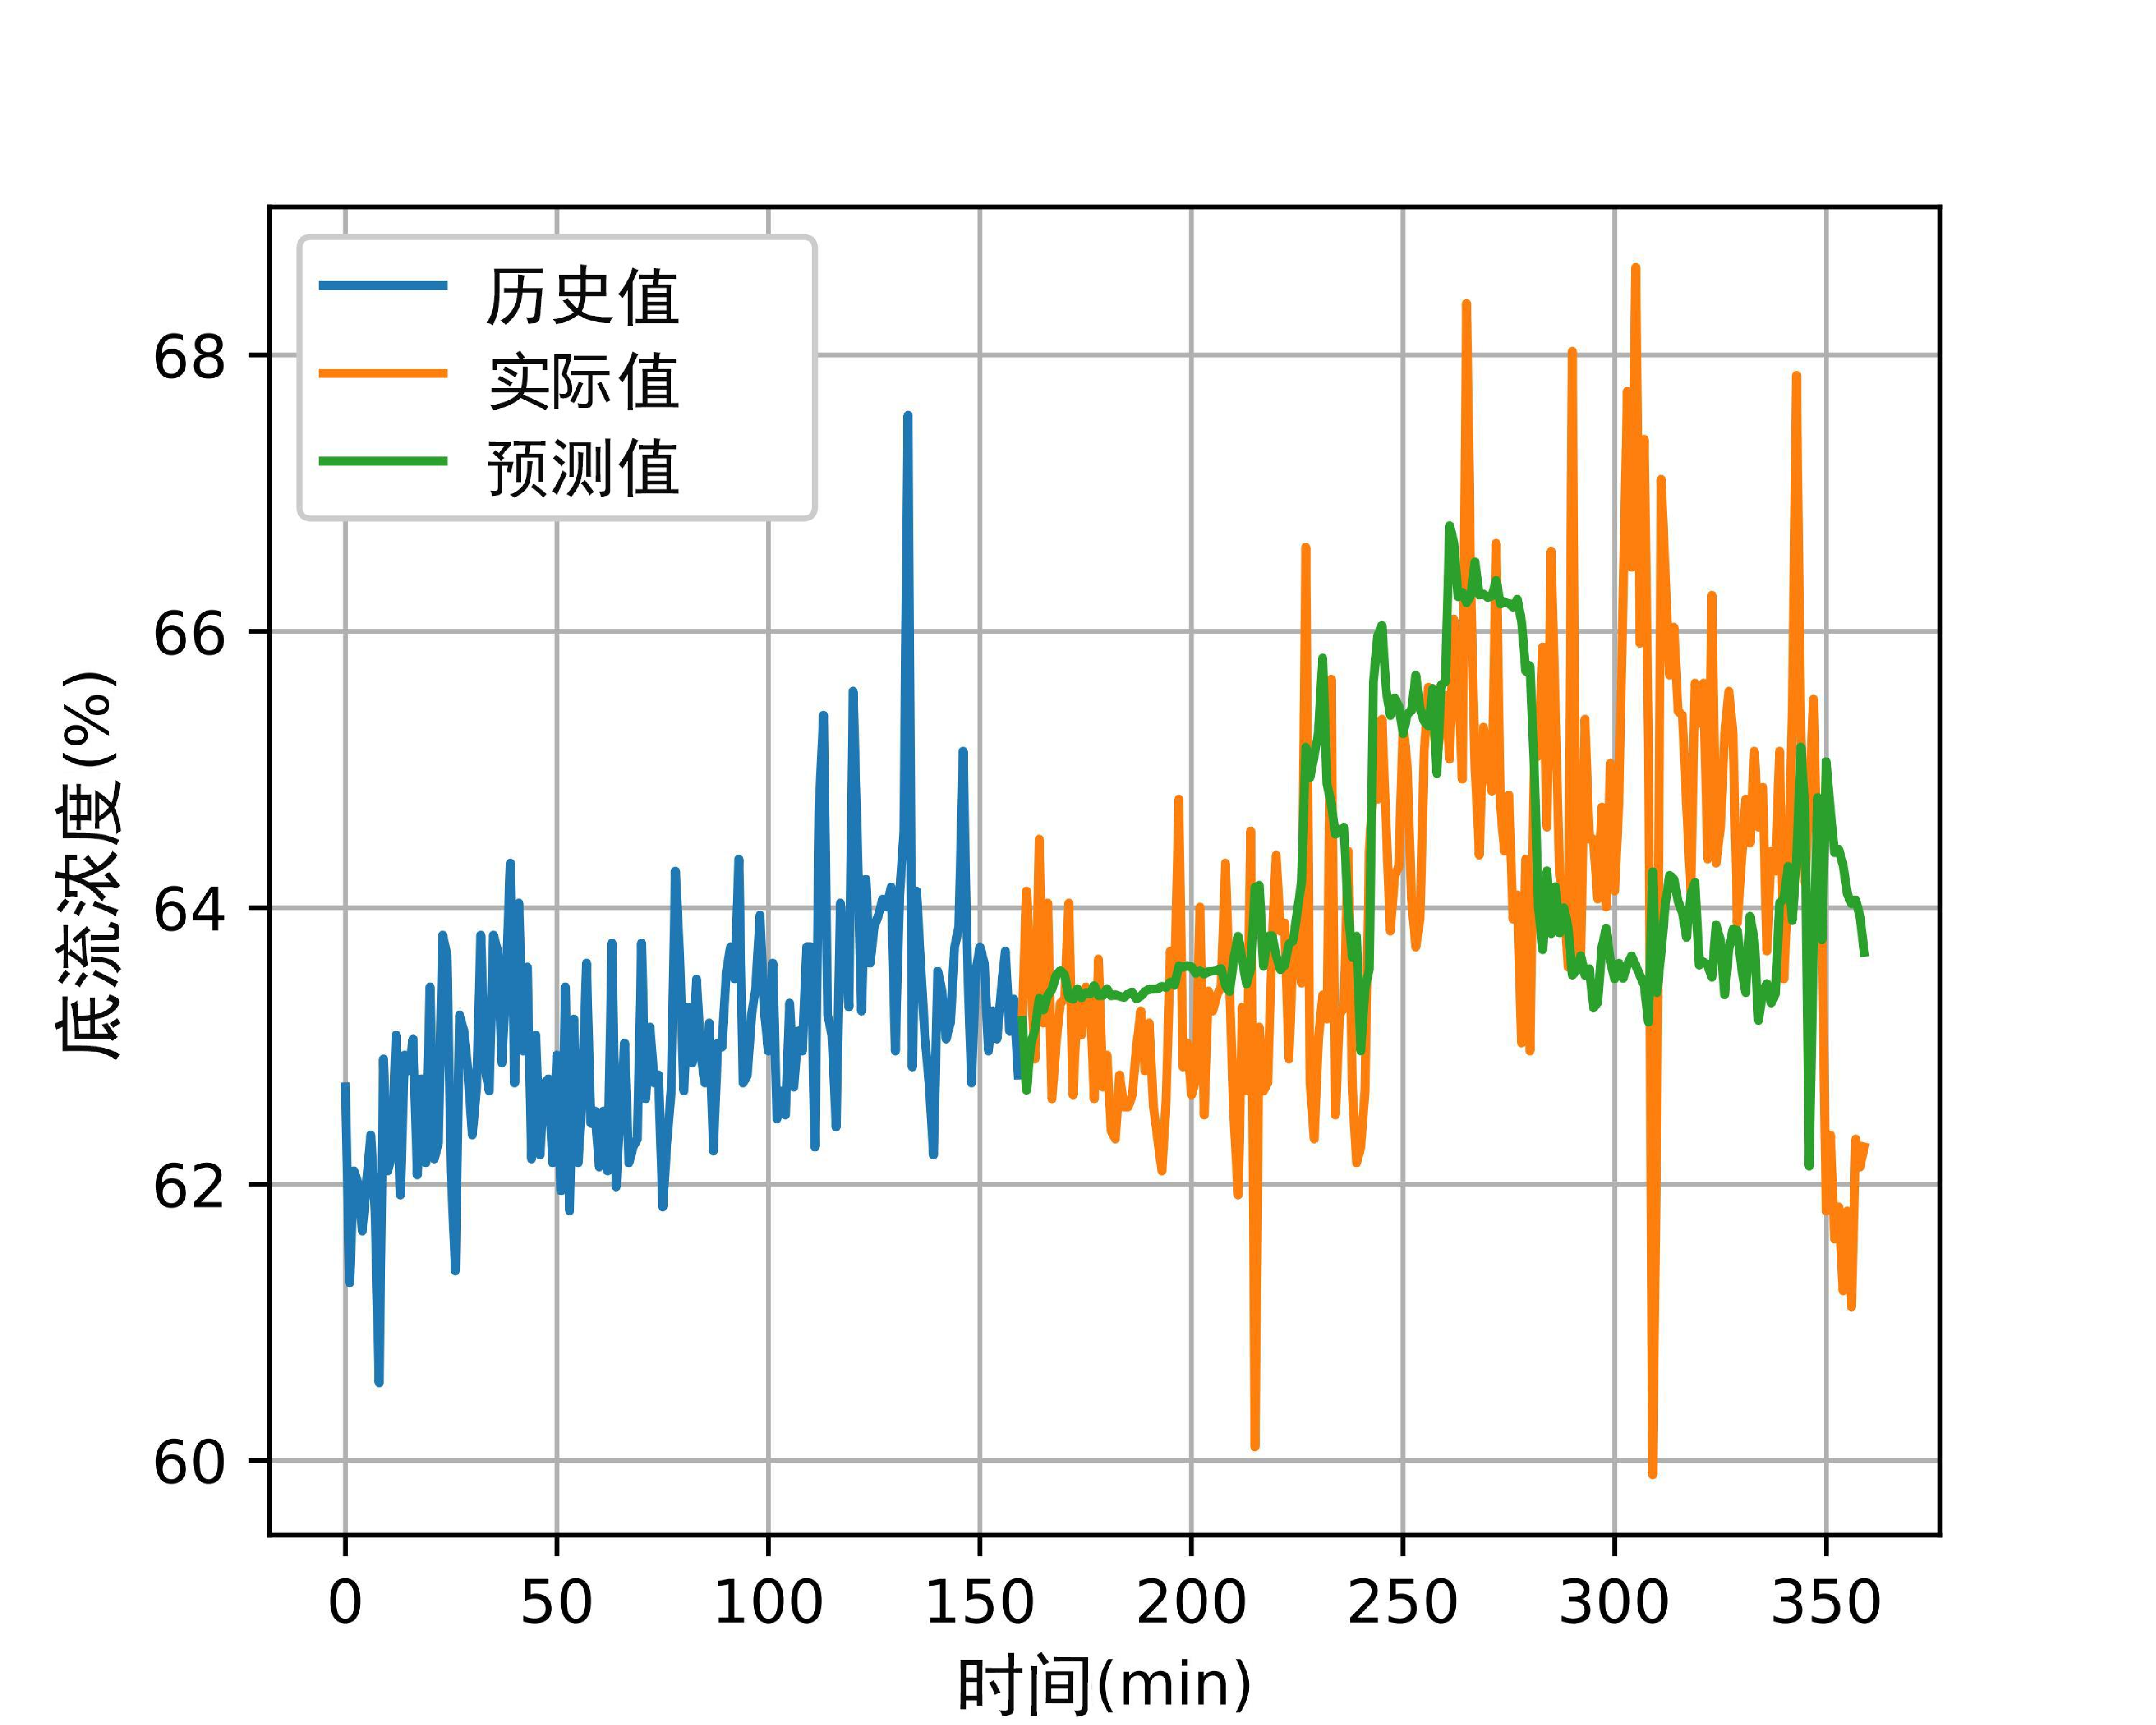
\includegraphics[width=0.45\linewidth,trim=50 0 0 200,clip]{figures/chapter3/predict_cmp/UC_GRU_sta_rk4_200.pdf}
%\caption{fig:subfig_200_sta_rk4}
\end{minipage}%
\label{fig:subfig_200_sta_rk4}
}%
% \subfigure[RNN-sta-Euler]{
% \begin{minipage}[t]{0.31\linewidth}
% \centering
% \includegraphics[width=1.1\linewidth]{figures/chapter3/predict_cmp/UC_RNN_sta_euler_200.eps}
% %\caption{fig2}
% \end{minipage}
% }%
\centering
\caption{$L=200$时不同ODE求解器、不同导数模块下的预测效果对比
} 
\label{fig:predict_cmp_200}
%\vspace*{-0.3cm}
\end{figure}
图中呈现的预测效果与表\ref{tab:3_exp_all}中的结果几乎一致。在长期预测任务中,非平稳模型的RRSE和MSE远远高于平稳模型,模型预测效果较差。
%It is meaningless to compare RRSE indices of results with different $L$, despite the RRSE in the experiments with $L=500$ is lower than $L=200$.
% When , we find that the model with stationary system performs lower prediction error than the non-stationary method.
% The illustrations of predicted results shown in Fig. \ref{fig:predict_cmp_200} and Fig. \ref{fig:predict_cmp_500} demonstrate that the non-stationary model only performs well in early period.
% The illustrations of predicted results shown in Fig. \ref{fig:predict_cmp_200} demonstrates that the non-stationary model only performs well in early period.
% We also illustrate the predicted results with $L=200$ in Fig. .
从图\ref{fig:predict_cmp_60}可以看出,非平稳模型在短期预测问题中展示了更好的预测效果。
而在图\ref{fig:predict_cmp_200}\subref{fig:subfig_200_nonsta_rk4}中,非稳定系统在长期预测时的预测精度显著衰减,且预测偏离程度伴随着预测序列长度的增加而增加。
与之相对地,稳定系统的预测结果是较为稳定的,更接近于系统的真实输出,证明稳定系统在长期预测中准确度更高。
% It is meaningless to compare RRSE indices of results with different $L$.
在由非稳定系统定义的导数模块中,其内部结构导致隐状态在积分过程中是无约束的,状态的取值范围将逐渐扩张。
虽然本章在状态解码器网络中嵌入$\tanh$函数,能够将预测的系统输出限制在合理的范围内,但解码器模块难以学习从极大的隐状态空间到系统输出空间的准确映射。

同样地,图~\ref{fig:predict_cmp_200}也证明了在长期预测问题中,高阶ODE求解器(如4阶Runge—Kutta)能够获得比低阶ODE求解器(如Euler)更好的预测效果,说明微分方程求解的精度会严重影响模型预测的精度,
结果与表\ref{tab:3_exp_all}一致。


% It notes that in the last part of simulation, the predicted system outputs deviate from the real sequences.
% The error is produced because thickening system is a partially observed system.
% Except for known external input or interference in $\b x(t)$, there exist plenty of invisible disturbances which affect the system extremely.
% The negative effects from unknown disturbances make the errors accumulated continuously over a long time period.
% In the long-term prediction task with $L=500$, the stationary model predicts the system outputs well in the former 300 minutes.




% TODO: 这部分也暂时注释,日后有机会再补上
%%%%%%%%%
% seek help: 自回归模型的缺点也是很明显的,每一轮循环的推理必须要在上一轮计算完成之后才能开始,ODE-Net也不例外
% The disadvantage of autogressive model is also obvious that, each round of recurrent inference has to done after the last round finished, and ode-net is no exception.
% One disadvantage for autoregressive model is the recurrent inference must follow by rounds, so does ODE-Net.
%%%%%%%%%

% 结果证实了基本rnn由于忽略了增稠系统的连续时间特性而不能很好地学习系统动力学方程的猜测。




本节额外进行了数组实验,以评估在其他预测长度$L$下,稳定系统和非稳定系统预测的底流浓度误差($\log_{10}{\text{MSE}}$)。
图~\ref{fig:length_cmp}展示了五次重复实验中,底流浓度的预测误差波动情况($\mu \pm 2\sigma$)。
虽然在短期预测任务中非稳定系统精度优于稳定系统,但当$L$超过$120$时,稳定系统表现更优。
% (如$L>100$)。
% 大约,非稳定系统的预测性能差于稳定系统。
\begin{figure}[h]
%\setlength{\abovecaptionskip}{-0.1cm} 
    \centering
    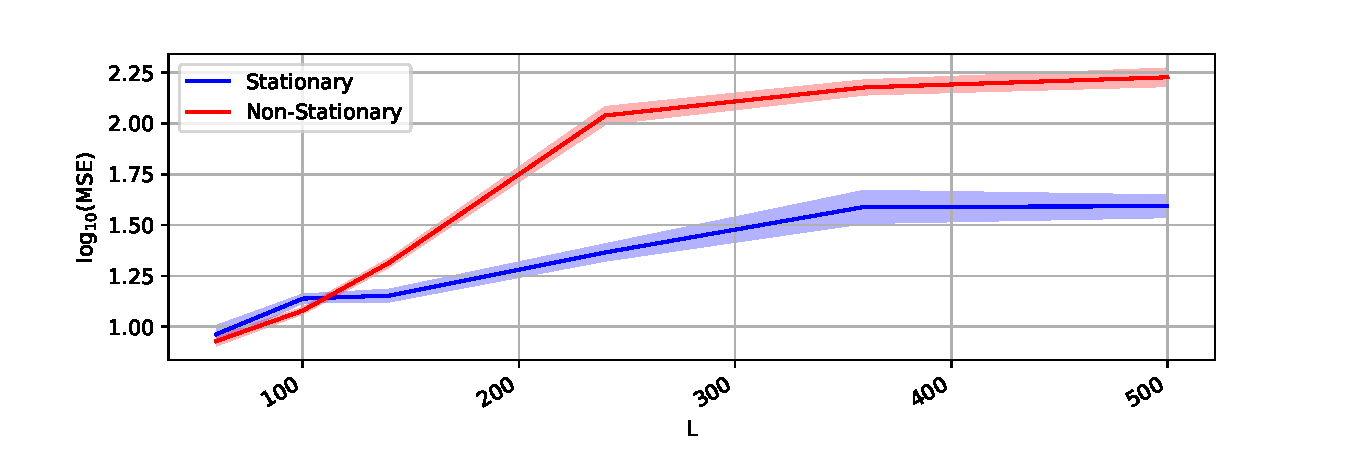
\includegraphics[width=\linewidth,trim=50 0 50 10, clip]{figures/chapter3/length_cmp.pdf}
    \caption{
    % The predicted length $L$ affects average $\log_{10}{MSE} \pm 2\sigma$ range of predicted underflow concentration for both stationary and non-stationary system.
    不同预测长度下稳定系统和非稳定系统的预测精度变化
    }
    \label{fig:length_cmp}
%\vspace*{-0.4cm}
\end{figure}




\subsection{序列编码器的有效性验证及系统时延探究}
\label{sec:3_enc_length}
最后,本节探究了引入序列编码器对于解决长时延系统预测问题的有效性。
% 具体地,该节对比了在引入序列编码器前后以及设定不同编码长度$N$对模型预测精度的影响。
具体地,该节对比了没有序列编码器,以及引入序列编码器并将编码长度$N$设置为不同值时,模型预测精度的变化情况。
特别地,当$N$设置为1时,将序列编码器替换为具有单一隐藏层的神经网络,该网络将单步系统输出$\b y(k-1)$及输入$\b x(k-1)$编码为ODE系统的初始隐状态$\b h(t_0)$。
当$N$为0时,初始状态$\b h(t_0)$被设定为可学习的初始隐状态\cite{Demeester2020SystemIW}或零向量,与历史系统轨迹无关。

% 在不同的预测序列长度$L=60$、$200$和$500$的三个实验中,我们测试了不同的$N$对预测精度的影响。
该实验仍然在$L=60$、$200$和$500$三种情况下比较不同初态估计方法对预测精度的影响。
在$L=60$的实验中,导数模块被为非平稳系统。
当$L=200$和$500$时,导数模块定义为带有GRU单元的稳定系统。
六组实验中,均采用四阶龙格-库塔求解器求解ODE方程。



\begin{table}[t]
\caption{不同初始隐状态 $\b h(t_0)$生成方法对于预测精度的影响}
\label{tab:seq2seq_cmp}
\centering
% \renewcommand{\arraystretch}{1.5}
\begin{tabular}{c|cc|cc|cc}
    \toprule
\multirow{2}{*}{$N$}                                                & \multicolumn{2}{c|}{\begin{tabular}[c]{@{}c@{}}$L=60$ \\ (120 分钟)\end{tabular}}                 & \multicolumn{2}{c|}{\begin{tabular}[c]{@{}c@{}}$L=200$ \\ (400 分钟)\end{tabular}}                  & \multicolumn{2}{c}{\begin{tabular}[c]{@{}c@{}}$L=500$ \\ (1000 分钟)\end{tabular}}                \\
\cline{2-7}
                                                                                     & RRSE                & MSE                 & RRSE                & MSE                  & RRSE                & MSE                  \\ \hline
160                                                                               & 3.11                & 9.08                &  \uline{\textbf{3.56}} & 34.13                & 1.61                & 35.88                \\
80                                                                                &  \uline{\textbf{3.10}} &  \uline{\textbf{8.97}} & 3.58                &  \uline{\textbf{32.92}} &  \uline{\textbf{1.61}} &  \uline{\textbf{34.88}} \\
40                                                                                & 3.19                & 8.99                & 3.65                & 36.07                & 1.71                & 41.26                \\ \hline
1                                                                                 & 4.06                & 10.71               & 4.97                & 51.09                & 1.77                & 63.56                \\ \hline
$N=0$,$\b h(t_0)$作为学习参数                  & 5.26                & 20.68               & 4.84                & 58.68                & 1.77                & 63.91                \\ \hline
$N=0$,令  $\b h(t_0)=\b 0$                                                                   & 5.26                & 23.11               & 5.84                & 64.49                & 1.77                & 63.53                \\ 
\bottomrule
\end{tabular}
\end{table}
从表\ref{tab:seq2seq_cmp}中的结果可以看出,相比于完全忽略历史系统输出($N=0$),引入序列编码器并利用历史运行轨迹构建常微分方程的初态能够获得更好的预测精度。
直觉上的解释为,待预测的系统未来输出与历史系统轨迹具有很强的统计相关性,从后者提取的特征对于序列预测具有重要意义。利用序列编码器能够将此部分相关性嵌入在ODE初态中。
根据实验发现,被编码序列的最优长度约为$N=80$,这与浓密机系统存在2至3小时时延的先验经验几乎一致。

另外,引入序列编码模块的收益在短期预测任务更加明显。
随着被预测序列长度的增加,引入序列编码器带来的优势也随之降低。

\subsection{探究序列插值阶数的对预测精度的影响}
% 本小节进行消融实验以探究不同离散输入序列进行插值的方法是否对预测精度产生影响。
本小节进行消融实验以探究不同离散输入序列插值方法对预测精度的影响。
测试对象包括四种不同阶数的样条插值方法,最终比较模型在不同预测长度的预测精度。
预测长度设置、导数形式、以及ODE求解器选择均与实验\ref{sec:3_enc_length}一致。
% The recurrent cell in experiment is RNN and the schema for solving ODE is RK4 uniformly.
表~\ref{tab:interolopation_cmp}所示结果表明,采用高阶样条插值时的精度将稍优于低阶插值。
\begin{table}[h]
\centering
%\setlength{\abovecaptionskip}{-0.1cm} 
\caption{不同序列插值方法对预测精度的影响}
\renewcommand{\arraystretch}{1.5}
\label{tab:interolopation_cmp}
\begin{tabular}{c|cc|cc|cc}
\toprule
 \multirow{2}{*}{模型}         & \multicolumn{2}{c|}{\begin{tabular}[c]{@{}c@{}}$L=60$ \\ (120 分钟)\end{tabular}}                 & \multicolumn{2}{c|}{\begin{tabular}[c]{@{}c@{}}$L=200$ \\ (400 分钟)\end{tabular}}                  & \multicolumn{2}{c}{\begin{tabular}[c]{@{}c@{}}$L=500$ \\ (1000 分钟)\end{tabular}}                 \\
    & RRSE                 & MSE                  & RRSE                 & MSE                   & RRSE                 & MSE                   \\ \hline
三次样条插值     &  \uline{\textbf{3.083}} & \uline{ \textbf{8.565}} & \uline{ \textbf{3.581}} & 32.90                & 1.615                & \uline{\textbf{ 34.88}} \\
二次样条插值 & 3.097                & 8.993                & 3.593                &\uline{ \textbf{32.585}} &\uline{ \textbf{1.613}} & 36.741                \\
线性插值   & 3.098                & 8.999                & 3.763                & 33.530                & 1.627                & 37.778                \\
零阶样条插值      & 3.115                & 9.050                & 3.791                & 33.585                & 1.628                & 37.695                \\ \bottomrule
\end{tabular}
%\vspace*{-0.4cm}
\end{table}
该结果说明本章所研究的膏体浓密机系统为复杂非线性受控系统,受控输入信息对于预测系统输出是十分重要的。
高阶样条插值方法能够更充分地利用相邻位置输入信号的相关特征,相比于低阶插值方法,能够更精确地对空白区域进行插值填充。

\section{本章小结}
\label{sec:conc}
本章针对高时延工业多输入输出系统预测问题,
提出了一种基于ODE-Net的连续时间网络模型,该模型由序列编码器、状态解码器和导数模块三部分组成,模型的内部计算过程包括历史序列编码、离散输入序列插值以及常微分方程求解三部分,模型能够从连续时间域角度拟合复杂系统的动态过程。
本章采用膏体浓密机系统运行数据集进行实验,以探究导数模块的不同定义方式、ODE求解器选择、离散序列插值阶数、序列编码长度对于预测精度的影响。
% 在真实膏体浓密机系统运行数据集,本章进行了大量实验对所提出模型的各个部分进行研究,包括平稳系统和非平稳系统的选择以及不同ODE求解器的设定。
结果表明,非平稳系统在短期预测任务中的表现优于平稳系统。
% 但是,非平稳模型由于存在累加计算,会造成隐状态的波动范围过大,进而导致长期预测性能较差。
在实际应用中,当构建基于模型的反馈控制器时,可使用非平稳系统作为短期预测模型辅助控制器输出。
但是,非平稳模型在长期预测时隐状态的波动范围过大且存在较大的累积误差,
而平稳系统通过修改导数模块结构,避免了隐状态漂移问题,因此在长期预测中表现较好。
当需要具有稳定鲁棒的系统识别模型进行长期预测时,如系统仿真或控制器测试,平稳系统模型是更好的选择。
同时,通过消融实验表明模型中引入序列编码器和并行三次样条插值能够有效改善模型精度。


% 在工业数据分析领域,面向不均匀采样数据的分析与预测是极其常见的。虽然本章所用数据集的采样间隔是均匀的,由于本文所述模型是基于ODE-Net进行构建的,具有连续时间域的系统学习及表示能力,因此该方法可以很自然地处理不均匀数据。
% 该问题值得在今后的工作中被进一步的验证。
% 另外将本章方法扩展为概率模型和时变模型,以辅助确定复杂系统中的未知噪音和不确定性,也是未来极具价值的研究方向。
